\documentclass[noglossariespages]{lapesd-thesis}

%%%%%%%%%%%%%%%%%%%%%%%%%%%%%%%%%%%%%%%%%%%%%%%%%%%%%%%%%%%%%%%%%%%%
%%% Dados do trabalho                                            %%%
%%%%%%%%%%%%%%%%%%%%%%%%%%%%%%%%%%%%%%%%%%%%%%%%%%%%%%%%%%%%%%%%%%%%

\titulo{Tolerância a Falhas Transparente para Aplicações MPI em Instâncias Spot
na Nuvem: Integração do MANA com o HPC@Cloud}
\autor{Artur Luiz Rizzato Toru Soda}
\data{2026}
\tcc
\departamento{Departamento de Informática e Estatística}
\curso{Ciências da Computação}
\titulode{Bacharel em Ciências da Computação}
\orientador{Prof. Márcio Bastos Castro, Dr.}

\membrobanca{Prof. Eduardo Camilo Inácio, Dr.}{Universidade Federal de Santa Catarina}
\membrobanca{Prof. Odorico Machado Mendizabal, Dr.}{Universidade Federal de Santa Catarina}
\coordenador{Prof.ª Lúcia Helena Martins Pacheco, Dr.ª}

\usepackage{amssymb}
\usepackage{tikz}
\usepackage{tabularx}

\makeindex

%%%%%%%%%%%%%%%%%%%%%%%%%%%%%%%%%%%%%%%%%%%%%%%%%%%%%%%%%%%%%%%%%%%%
%%% Lista de siglas                                              %%%
%%% IMPORTANTE: a lista PRECISA SER MANTIDA ORDENADA            %%%
%%%%%%%%%%%%%%%%%%%%%%%%%%%%%%%%%%%%%%%%%%%%%%%%%%%%%%%%%%%%%%%%%%%%

\xnewacronym{AMI}{Amazon Machine Image}
\xnewacronym{ANN}{Artificial Neural Network}
\xnewacronym{API}{Application Programming Interface}
\xnewacronym{AWS}{Amazon Web Services}
\xnewacronym{BLCR}{Berkeley Lab Checkpoint/Restart}
\xnewacronym{BU}{Biblioteca Universitária}
\xnewacronym{CFD}{Computational Fluid Dynamics}
\xnewacronym{CG}{Conjugate Gradient}
\xnewacronym{CPU}{Central Processing Unit}
\xnewacronym{DMTCP}{Distributed MultiThreaded CheckPointing}
\xnewacronym{EC2}{Amazon Elastic Compute Cloud}
\xnewacronym{EFA}{Elastic Fabric Adapter}
\xnewacronym{EFS}{Amazon Elastic File System}
\xnewacronym{EIP}{Elastic IP Address}
\xnewacronym{EP}{Embarrassingly Parallel}
\xnewacronym{FT}{Fault Tolerant}
\xnewacronym{HPC}{High-Performance Computing}
\xnewacronym{IaaS}{Infrastructure as a Service}
\xnewacronym{LU}{Lower-Upper Symmetric Gauss-Seidel}
\xnewacronym{MANA}{MPI-Agnostic, Network-Agnostic}
\xnewacronym{MPI}{Message Passing Interface}
\xnewacronym{MTBF}{Mean Time Between Failures}
\xnewacronym{MTTF}{Mean Time To Failure}
\xnewacronym{MTTR}{Mean Time To Recovery}
\xnewacronym{NIST}{National Institute of Standards and Technology}
\xnewacronym{NPB}{NAS Parallel Benchmarks}
\xnewacronym{PaaS}{Platform as a Service}
\xnewacronym{PIBIC}{Programa Institucional de Bolsas de Iniciação Científica}
\xnewacronym{SaaS}{Software as a Service}
\xnewacronym{SCR}{Scalable Checkpoint/Restart}
\xnewacronym{SLA}{Service Level Agreement}
\xnewacronym{SLURM}{Simple Linux Utility for Resource Management}
\xnewacronym{SSM}{AWS Systems Manager Session Manager}
\xnewacronym{TCC}{Trabalho de Conclusão de Curso}
\xnewacronym{ULFM}{User-Level Failure Mitigation}
\xnewacronym{VM}{Virtual Machine}

%%% Local Variables:
%%% mode: latex
%%% TeX-master: "main"
%%% End:

\input{glossary.tex}

\begin{document}

\pretextual%
% Assume-se que \pretextual já foi feito

\imprimircapa%
\imprimirfolhaderosto*
% \protect\incluirfichacatalografica{ficha.pdf}  % descomentar quando tiver a ficha
{}% placeholder: evita que \imprimirfolhadecertificacao seja engolido pelo \@ifstar
\imprimirfolhadecertificacao


% \begin{dedicatoria}
% \end{dedicatoria}


\begin{agradecimentos}
Ao Prof.\ Márcio Bastos Castro, pela orientação cuidadosa, pela liberdade de
exploração e pelo ambiente de pesquisa que tornou este trabalho possível.

Ao LaPeSD, em especial a Vanderlei Munhoz, cujo desenvolvimento do orquestrador
HPC@Cloud serviu de base para a integração proposta neste trabalho, e cujas
contribuições técnicas ao longo do projeto foram determinantes.

Este trabalho foi parcialmente financiado pelo Conselho Nacional de
Desenvolvimento Científico e Tecnológico (CNPq) e pela Amazon Web Services
(AWS) por meio da Chamada CNPq/AWS Nº~64/2022 (Cloud Credits for Research).

À minha família, pelo apoio incondicional ao longo de toda a graduação.
\end{agradecimentos}


% \begin{epigrafe}
% \end{epigrafe}


\begin{resumo}[Resumo]
Instâncias \textit{spot} da Amazon Web Services oferecem descontos de até 90\%
em relação ao preço convencional, mas podem ser revogadas pelo provedor a
qualquer momento, com aviso de apenas dois minutos, descartando todo o progresso
computacional acumulado em aplicações MPI de longa duração. Este trabalho propõe
e avalia uma arquitetura de execução resiliente para aplicações MPI legadas em
instâncias \textit{spot}, sem exigir modificação de código, por meio da
integração do MANA, sistema de \textit{checkpoint/restart} transparente para MPI,
ao orquestrador HPC@Cloud. A topologia adotada é híbrida: nó coordenador em
instância \textit{burstable on-demand} e nós de computação em instâncias
\textit{spot}. Duas estratégias de recuperação são implementadas: a
\textsc{Replace}, que reprovísiona o nó interrompido e retoma a execução com a
capacidade original do \textit{cluster}, e a \textsc{Degraded}, que marca o nó
como inativo e reinicia imediatamente com $N{-}1$ \textit{workers}. A avaliação
experimental, conduzida com 282 execuções sobre os \textit{benchmarks} NPB
CG-C, EP-D e LU-C em \textit{clusters} de 2, 4 e 8 \textit{workers}, revelou
dois regimes de viabilidade: para \textit{jobs} curtos como o CG-C (12 a 35~s),
o \textit{overhead} de recuperação domina e a abordagem não se justifica; para
\textit{jobs} de duração moderada a longa como o EP-D e o LU-C, a
\textsc{Degraded} alcançou menor tempo de execução em 17 das 18 configurações
avaliadas, com economia de custo de 2 a 38\% em relação à execução equivalente
em instâncias \textit{on-demand} sem tolerância a falhas.

\vspace{\baselineskip}
\textbf{Palavras-chave:} Computação em Nuvem. Computação de Alto Desempenho.
Instâncias \textit{Spot}. Tolerância a Falhas. \textit{Checkpoint/Restart}.
MANA. HPC@Cloud.
\end{resumo}


\begin{resumo}[Resumo Estendido]

\section*{Introdução}

A computação de alto desempenho (HPC) tem migrado progressivamente para
ambientes de nuvem pública, atraída pela elasticidade de recursos e pelo modelo
de cobrança por uso. Nesse contexto, as instâncias \textit{spot} da Amazon Web
Services representam uma oportunidade econômica relevante: ao adquirir
capacidade computacional ociosa do provedor, é possível obter descontos de até
90\% em relação ao preço convencional. Essa vantagem de custo, contudo, vem
acompanhada de uma restrição operacional significativa: o provedor pode revogar
as instâncias \textit{spot} a qualquer momento, com aviso mínimo de dois
minutos antes da terminação efetiva.

Para aplicações de curta duração, a probabilidade de interrupção é baixa e o
impacto de uma revogação é tolerável. Para aplicações MPI de longa duração,
porém, uma revogação descarta todo o progresso computacional acumulado, forçando
a reexecução completa do \textit{job}. Essa característica torna as instâncias
\textit{spot} impraticáveis para esse tipo de carga sem um mecanismo de
preservação de estado, especialmente quando as aplicações são legadas e não
preveem modificação de código.

O MANA (\textit{MPI-Agnostic Network-Agnostic checkpoint/restart}) é um sistema
de \textit{checkpoint} transparente para aplicações MPI que opera sem qualquer
modificação no código da aplicação. Baseado no DMTCP (\textit{Distributed
MultiThreaded CheckPointing}), o MANA captura a imagem completa do estado de
execução de todos os processos MPI e permite retomá-la a partir do ponto salvo,
mesmo após uma falha de nó. Essa propriedade cria a oportunidade de combinar a
economia das instâncias \textit{spot} com a resiliência necessária para
\textit{jobs} de longa duração.

Este trabalho integra o MANA ao orquestrador HPC@Cloud para construir uma
arquitetura de execução resiliente e econômica para aplicações MPI legadas em
instâncias \textit{spot}. A questão central investigada é se e quando essa
combinação é viável, tanto em termos de tempo de execução quanto de custo
monetário, em comparação com a alternativa de instâncias \textit{on-demand} sem
tolerância a falhas.


\section*{Objetivos}

O objetivo geral deste trabalho é propor, implementar e avaliar uma arquitetura
de execução resiliente e econômica para aplicações HPC em instâncias
\textit{spot} da AWS, integrando o MANA ao HPC@Cloud e quantificando o impacto
em desempenho e custo em comparação com execução nativa sem tolerância a falhas.

Os objetivos específicos são:
\begin{enumerate}
  \item Consolidar a análise de viabilidade de instâncias \textit{burstable}
        para HPC em nuvem, identificando seus limites operacionais e justificando
        seu uso restrito ao papel de coordenador de \textit{checkpoint};
  \item Estender o HPC@Cloud com suporte à topologia híbrida
        \textit{head}/\textit{worker}, incluindo diferenciação de papéis por
        tipo de instância e as implicações no processo de provisionamento;
  \item Implementar o \textit{bootstrap} automatizado do ambiente MANA/DMTCP
        sobre \textit{clusters} AWS, incluindo configuração do Slurm,
        implantação dos binários MANA e sincronização de estado via EFS;
  \item Implementar um mecanismo de detecção de interrupção e duas estratégias
        de recuperação (\textsc{Replace} e \textsc{Degraded}), com suporte a
        falhas sintéticas reproduzíveis para fins de avaliação controlada;
  \item Quantificar o \textit{overhead} do MANA sobre os NAS Parallel
        Benchmarks (NPB), especificamente CG-C, EP-D e LU-C, em
        \textit{clusters} com 2, 4 e 8 \textit{workers}, incluindo estudos
        sintéticos para isolar os mecanismos de \textit{overhead};
  \item Comparar o custo-benefício das estratégias \textsc{Replace} e
        \textsc{Degraded} em relação à execução nativa, identificando as
        condições sob as quais cada estratégia é economicamente vantajosa.
\end{enumerate}


\section*{Metodologia}

A topologia adotada é híbrida: um nó coordenador (\textit{head}) opera como
instância t3.large \textit{on-demand}, imune a revogações, e os nós de
computação (\textit{workers}) executam como instâncias m5.xlarge \textit{spot},
aproveitando os descontos de até 90\%. Essa escolha foi fundamentada na análise
de viabilidade de instâncias \textit{burstable} conduzida previamente, que
demonstrou que o perfil intermitente do coordenador de \textit{checkpoint} é
compatível com as limitações de CPU e rede dessas instâncias, enquanto cargas
HPC com sincronização frequente sofrem degradação expressiva.

A integração ao HPC@Cloud implementa três componentes. O \textit{bootstrap}
automatizado configura o ambiente Slurm e implanta os binários do MANA no EFS
compartilhado, tornando os nós operacionais sem intervenção manual. O
\textit{watcher} monitora periodicamente o estado das instâncias \textit{spot}
via API da EC2 e, ao detectar uma revogação iminente, aciona o salvamento do
estado de todos os processos MPI. Após a confirmação do
\textit{checkpoint}, o sistema aplica uma das duas estratégias configuráveis: a
\textsc{Replace}, que reprovísiona o nó interrompido e retoma o \textit{job}
com a capacidade original do \textit{cluster}, e a \textsc{Degraded}, que marca
o nó como inativo e reinicia imediatamente com $N{-}1$ \textit{workers}.

Para isolar cada componente do custo de recuperação, a execução é decomposta em
quatro fases: P0 (computação antes da falha), P1 (escrita do
\textit{checkpoint}), P2 (reconfiguração do nó, subdividida em P2a$+$P2c
comuns às duas estratégias e P2b onde elas divergem) e P3 (computação após o
reinício). Essa decomposição permite atribuir cada segundo observado a uma causa
específica, separando tempo de computação de tempo de infraestrutura e de
coordenação.

A avaliação experimental utilizou os \textit{benchmarks} NPB CG-C
(\textit{Conjugate Gradient}, classe~C), EP-D (\textit{Embarrassingly Parallel},
classe~D) e LU-C (\textit{Lower-Upper Gauss-Seidel}, classe~C), representando
respectivamente regimes de comunicação intensiva com buffers por processo,
operações coletivas sem estado por \textit{rank} e comunicação estruturada com
vizinhos de cardinalidade fixa. A matriz de experimentos combinou 3
\textit{benchmarks} por 3 tamanhos de \textit{cluster} (2, 4 e 8
\textit{workers}) por 3 momentos de falha (10\%, 25\% e 50\% do tempo total)
por 2 estratégias, além das linhas de base noFT e MANA-noFT, totalizando 282
execuções válidas com $N{=}3$ repetições por configuração. A injeção de falhas
foi realizada de forma sintética e reproduzível por meio do mecanismo
\texttt{auto\_test\_failure} do HPC@Cloud.


\section*{Resultados e Discussão}

A avaliação revelou que o \textit{overhead} do MANA em condições normais
(sem falhas) é aplicação-dependente e emerge da interação entre o padrão de
execução de cada aplicação e a camada de instrumentação do MANA: varia de 27\%
no EP-D com 8~\textit{workers} a 222\% no CG-C com 2~\textit{workers}. Os
estudos sintéticos identificaram que a frequência de chamadas MPI não é o
mecanismo amplificador; o custo intrínseco medido em programas isolados é de
apenas 4 a 5~s por execução. A distância entre esse valor e os percentuais
observados nos \textit{benchmarks} reais indica que o \textit{overhead} relevante
é específico ao padrão de execução de cada aplicação.

A análise das fases de recuperação revelou onde as estratégias divergem: a fase
P2b, que compreende a reconfiguração do nó após a falha. A \textsc{Degraded}
conclui P2b em $\approx$11~s ao atualizar o estado do nó no Slurm; a
\textsc{Replace} aguarda $\approx$120~s pelo reaprovisionamento de um nó
substituto na AWS. Essa diferença de $\approx$109~s é o elemento central da
comparação entre estratégias, e seu peso relativo é modulado por dois fatores
que interagem: o tamanho do \textit{cluster} ($N$) e o volume de trabalho
remanescente no momento da falha.

Em \textit{clusters} maiores, a perda de um nó representa uma fração menor da
capacidade total, reduzindo a penalidade de P3 da \textsc{Degraded} e tornando
a economia de P2b dominante. Em \textit{clusters} pequenos com falha precoce, o
custo de P3 com $N{-}1$ \textit{workers} pode superar os $\approx$109~s
economizados, tornando a \textsc{Replace} mais eficiente. Essa estrutura de
\textit{crossover} foi observada empiricamente em apenas um dos 18 cenários
avaliados para EP-D e LU-C: o EP-D com 2~\textit{workers} e falha a 10\% do
tempo total. Nas demais 17 configurações, a \textsc{Degraded} apresentou menor
tempo de execução, com vantagem crescente conforme $N$ aumenta.

Os resultados revelam dois regimes econômicos distintos. Para \textit{jobs}
curtos como o CG-C (12 a 35~s), o \textit{overhead} de recuperação equivale a
3 a 17 vezes o tempo útil de cálculo, e o desconto \textit{spot} não compensa
nem em tempo nem em custo. Para \textit{jobs} de duração moderada a longa como
o EP-D e o LU-C, a \textsc{Degraded} alcança economia de 2 a 38\% em relação
ao equivalente \textit{on-demand} sem recuperação, com as análises de tempo e
de custo apontando consistentemente na mesma direção. A viabilidade depende,
portanto, de forma determinante da duração do \textit{job}: apenas quando o
custo fixo de recuperação representa uma fração minoritária do tempo total é que
a combinação de \textit{spot} com tolerância a falhas se torna vantajosa.


\section*{Considerações Finais}

A integração proposta demonstra que execução resiliente e econômica de
aplicações MPI legadas em instâncias \textit{spot} é alcançável sem modificação
de código, desde que a duração do \textit{job} seja suficiente para amortizar o
custo de recuperação. Os seis objetivos específicos foram atendidos: a análise
de instâncias \textit{burstable} fundamentou a topologia adotada; o HPC@Cloud
foi estendido com \textit{bootstrap} automatizado e dois mecanismos de
recuperação configuráveis; e a avaliação experimental quantificou o
\textit{overhead}, caracterizou o comportamento das estratégias e identificou as
condições de viabilidade econômica.

Como extensões naturais do trabalho, destacam-se: a validação empírica do regime
de \textit{jobs} de longa duração, com classes mais custosas dos
\textit{benchmarks}, observando a restrição do limite de dois minutos para
escrita do \textit{checkpoint}; a avaliação do comportamento das estratégias
sob múltiplas falhas sequenciais; e a adição de \textit{checkpoints} periódicos
combinados com predição de revogações baseada em histórico de interrupções de
instâncias \textit{spot}.

\vspace{\baselineskip}
\textbf{Palavras-chave:} Computação em Nuvem. Computação de Alto Desempenho.
Instâncias \textit{Spot}. Tolerância a Falhas. \textit{Checkpoint/Restart}.
MANA. HPC@Cloud.
\end{resumo}


\begin{abstract}
AWS spot instances offer discounts of up to 90\% compared to on-demand pricing,
but may be revoked by the provider at any time with only two minutes of notice,
discarding all accumulated computational progress in long-running MPI
applications. This work proposes and evaluates a resilient execution
architecture for legacy MPI applications on AWS spot instances, without
requiring code modification, by integrating MANA, a transparent
\textit{checkpoint/restart} system for MPI, with the HPC@Cloud orchestrator.
The adopted topology is hybrid: a coordinator node on a \textit{burstable
on-demand} instance and compute nodes on \textit{spot} instances. Two recovery
strategies are implemented: \textsc{Replace}, which reprovisions the interrupted
node and resumes execution with the original cluster capacity, and
\textsc{Degraded}, which marks the node as inactive and immediately restarts
with $N{-}1$ workers. The experimental evaluation, conducted with 282 executions
on the NPB benchmarks CG-C, EP-D, and LU-C on clusters of 2, 4, and 8 workers,
revealed two viability regimes: for short jobs such as CG-C (12 to 35~s),
recovery overhead dominates and the approach is not worthwhile; for medium to
long-running jobs such as EP-D and LU-C, \textsc{Degraded} achieved shorter
execution times in 17 out of 18 evaluated configurations, with cost savings of
2 to 38\% compared to the equivalent on-demand execution without fault
tolerance.

\vspace{\baselineskip}
\textbf{Keywords:} Cloud Computing. High Performance Computing. Spot Instances.
Fault Tolerance. Checkpoint/Restart. MANA. HPC@Cloud.
\end{abstract}


\listoffigures*
\listoftables*
\listofalgorithms*

%%% Força todas as siglas definidas em acronyms.tex a aparecer na lista,
%%% mesmo sem uso de \gls{} no texto.
\glsaddall
\listadesiglas*[7em]

\tableofcontents*%

%%% Local Variables:
%%% mode: latex
%%% TeX-master: "main"
%%% End:

\textual%
% Assume-se que \textual já foi feito

% ==========================================================================
\chapter{Introdução}
\label{ch:introducao}
% ==========================================================================

A migração de cargas de trabalho de Computação de Alto Desempenho (HPC) para a nuvem
tem se intensificado ao longo da última década, impulsionada pelo acesso sob demanda a
recursos computacionais de larga escala sem os custos de capital de infraestrutura
física~\cite{mell2011nist,gartner2022iaas}. Provedores como a Amazon Web Services (AWS)
disponibilizam \textit{clusters} virtuais configuráveis com dezenas de vCPUs e alta capacidade
de memória sob o modelo \textit{pay-as-you-go}, tornando a nuvem uma alternativa
economicamente acessível para aplicações científicas e de engenharia em
escala~\cite{netto2018hpccloud}.


Entre os modelos de precificação disponíveis, as instâncias \textit{spot} representam
a alternativa de menor custo: disponibilizam capacidade computacional ociosa do provedor
com descontos de até 90\% em relação ao preço convencional~\cite{aws2018spot}, tornando-as
especialmente atrativas para \textit{workloads} HPC de longa duração. O modelo
\textit{spot} implica, porém, um risco fundamental: a instância pode ser revogada a
qualquer momento, com apenas dois minutos de aviso prévio~\cite{aws2026spot_termination},
quando o provedor precisar recuperar a capacidade. Para aplicações MPI de longa duração
(como simulações numéricas que levam horas ou dias), uma interrupção sem salvamento de
estado implica a perda de todo o progresso computacional acumulado desde o início do
\textit{job}.

A solução clássica para esse problema é o mecanismo de \textit{checkpoint/restart}:
salvar periodicamente o estado completo de todos os processos em armazenamento
persistente, de modo que um \textit{job} interrompido possa ser retomado a partir do
último ponto salvo em vez de reiniciar do zero~\cite{hargrove2006blcr,moody2010scr}.
No entanto, adicionar \textit{checkpoint/restart} a aplicações MPI existentes
tipicamente exige modificações no código-fonte, limitando a adoção em aplicações
científicas legadas que não foram projetadas com tolerância a falhas em mente. O
\textit{checkpoint/restart} transparente, em que a aplicação não precisa ser
alterada, configura-se, portanto, como a abordagem ideal para viabilizar a recuperação
sem onerar os desenvolvedores.

O MANA (\textit{MPI-Agnostic, Network-Agnostic transparent checkpointing})%
~\cite{garg2019mana,arya2016split}, desenvolvido sobre o framework DMTCP
(\textit{Distributed MultiThreaded CheckPointing})~\cite{ansel2009dmtcp}, oferece
exatamente essa propriedade: salvamento e restauração transparentes do estado de
aplicações MPI, independentemente da implementação MPI utilizada ou do tipo de rede
subjacente. A independência de rede é particularmente relevante no contexto de nuvem,
onde instâncias \textit{spot} substituídas recebem novos endereços IP após cada
provisionamento, o que inviabiliza abordagens de \textit{checkpoint} acopladas a
endereços de rede fixos.

Um estudo anterior do presente autor~\cite{soda2025erad,soda2025wcc} caracterizou o
desempenho de instâncias \textit{burstable} (família T3) da AWS em cargas de trabalho
HPC. Instâncias \textit{burstable} utilizam um sistema de créditos de CPU que permite
rajadas de desempenho completo por períodos limitados, seguidas de \textit{throttling}
quando os créditos se esgotam. Os resultados demonstraram que essas instâncias são
inadequadas como nós de computação para \textit{benchmarks} MPI intensivos em CPU, mas possuem
um perfil de consumo intermitente de CPU compatível com o papel de coordenador do
mecanismo de \textit{checkpoint}, responsável por gerenciar o processo de salvamento
de estado, mas que não realiza computação científica.

Esses achados motivaram a arquitetura proposta neste trabalho: uma topologia híbrida
composta por instâncias \textit{spot} como nós de computação, adquiridas ao preço
\textit{spot} com desconto de até 90\%~\cite{aws2018spot} em relação ao valor sob
demanda, e por uma instância \textit{burstable on-demand} como nó coordenador do
MANA/DMTCP, responsável pela estabilidade do processo de \textit{checkpoint} a custo
residual mínimo. O orquestrador HPC@Cloud~\cite{munhoz2024hpccloud} automatiza o provisionamento
do \textit{cluster}, a detecção de falhas e o reinício dos \textit{jobs}, abstraindo a
complexidade de gerenciar a infraestrutura de \textit{checkpoint} sobre instâncias
transitórias. Duas estratégias de recuperação são implementadas e avaliadas neste
trabalho: \textsc{Replace}, que substitui o nó falho e retoma o \textit{job} com o paralelismo
original, e \textsc{Degraded}, que reinicia imediatamente com um processo a menos,
priorizando a minimização do tempo de inatividade.


\section{Objetivos}
\label{sec:objetivos}

\subsection{Objetivo Geral}
\label{sec:objetivo-geral}

Propor, implementar e avaliar uma arquitetura de execução resiliente e econômica para
aplicações HPC em instâncias \textit{spot} da AWS, integrando o mecanismo de
\textit{checkpoint/restart} transparente MANA ao orquestrador HPC@Cloud e
quantificando o impacto em desempenho e custo monetário em comparação com execução
nativa sem tolerância a falhas.


\subsection{Objetivos Específicos}
\label{sec:objetivos-especificos}

\begin{enumerate}
  \item Consolidar a análise de viabilidade de instâncias \textit{burstable} para HPC
        em nuvem, identificando seus limites operacionais e justificando seu uso
        restrito ao papel de coordenador de \textit{checkpoint};
  \item Estender o HPC@Cloud com suporte à topologia híbrida
        \textit{head}/\textit{worker}, incluindo diferenciação de papéis por tipo de
        instância e as implicações no processo de provisionamento automatizado;
  \item Implementar o \textit{bootstrap} automatizado do ambiente MANA/DMTCP sobre
        \textit{clusters} AWS, incluindo configuração do Slurm, implantação dos binários MANA
        e sincronização de estado via Amazon Elastic File System (EFS);
  \item Implementar um mecanismo de detecção de interrupção e as duas estratégias de
        recuperação (\textsc{Replace} e \textsc{Degraded}), com suporte a falhas
        sintéticas reproduzíveis para fins de avaliação controlada;
  \item Quantificar o \textit{overhead} do MANA sobre os NAS Parallel Benchmarks (NPB),
        especificamente CG-C, EP-D e LU-C, em \textit{clusters} com 2, 4 e 8 \textit{workers}, incluindo
        estudos sintéticos para isolar os mecanismos de \textit{overhead};
  \item Comparar o custo-benefício das estratégias \textsc{Replace} e \textsc{Degraded}
        em relação à execução nativa, identificando as condições sob as quais cada
        estratégia é economicamente vantajosa.
\end{enumerate}


\section{Contribuições}
\label{sec:contribuicoes}

As principais contribuições deste trabalho são:

\begin{itemize}
  \item \textbf{Projeto e implementação de uma arquitetura de execução resiliente para
        aplicações MPI legadas em instâncias \textit{spot}:} topologia híbrida com nó
        coordenador \textit{on-demand} e \textit{workers spot}, \textit{bootstrap}
        automatizado do ambiente MANA/Slurm sobre Amazon EFS e mecanismo de detecção
        de interrupção com \textit{checkpoint} reativo, sem exigir modificação nas
        aplicações;

  \item \textbf{Projeto e avaliação de duas estratégias de recuperação para
        aplicações MPI interrompidas em instâncias \textit{spot}:} exploração do
        \textit{trade-off} entre restauração da capacidade computacional original
        (\textsc{Replace}) e retomada imediata da execução com \textit{cluster} reduzido
        (\textsc{Degraded}), com caracterização das condições temporais e econômicas que
        determinam a preferência entre as estratégias;

  \item \textbf{Avaliação experimental sistemática do \textit{overhead} e do
        custo-benefício da arquitetura proposta:} 282~execuções sobre os NAS Parallel
        Benchmarks CG-C, EP-D e LU-C em \textit{clusters} de 2, 4 e 8
        \textit{workers}, identificando os regimes de duração de \textit{job} nos quais
        a combinação de instâncias \textit{spot} com \textit{checkpoint/restart}
        transparente é economicamente vantajosa em relação à execução nativa sob
        demanda.
\end{itemize}


\section{Organização do Trabalho}
\label{sec:organizacao}

O restante deste trabalho está organizado da seguinte forma. O
Capítulo~\ref{ch:fundamentacao} apresenta a fundamentação teórica, cobrindo computação
em nuvem, HPC, tolerância a falhas, o framework DMTCP, o MANA, o HPC@Cloud e os NAS
Parallel Benchmarks. O Capítulo~\ref{ch:relacionados} discute os trabalhos relacionados
nas dimensões de tolerância a falhas em MPI, HPC em instâncias \textit{spot} e predição
de falhas em nuvem, posicionando este trabalho frente à literatura. O
Capítulo~\ref{ch:burstable} apresenta a análise de viabilidade de instâncias
\textit{burstable}, trabalho anterior que motivou a topologia híbrida adotada. O
Capítulo~\ref{ch:implementacao} descreve em detalhes a implementação da arquitetura
proposta no HPC@Cloud. O Capítulo~\ref{ch:avaliacao} apresenta a avaliação
experimental completa, com 282 execuções distribuídas em estudos de \textit{overhead}, tamanho
de \textit{checkpoint}, sensibilidade ao momento da falha e comparação de estratégias.
O Capítulo~\ref{ch:conclusao} sintetiza as contribuições do trabalho e aponta direções
para pesquisas futuras.


% ==========================================================================
\chapter{Fundamentação Teórica}
\label{ch:fundamentacao}
% ==========================================================================

Três camadas conceituais sustentam a arquitetura proposta neste trabalho: a
infraestrutura de nuvem que provê os recursos computacionais
(Seção~\ref{sec:cloud}), os ambientes de execução paralela distribuída que os
exploram (Seção~\ref{sec:hpc}), e os mecanismos de tolerância a falhas que
protegem o progresso computacional (Seção~\ref{sec:fault-tolerance}). O
orquestrador HPC@Cloud (Seção~\ref{sec:hpcac}) integra essas três camadas em um
fluxo automatizado, e os NAS Parallel Benchmarks (Seção~\ref{sec:npb}) constituem
o instrumento de avaliação experimental adotado.

\section{Computação em Nuvem}
\label{sec:cloud}

O \textit{National Institute of Standards and Technology} (NIST) define computação
em nuvem como um modelo que viabiliza acesso global, conveniente e sob demanda a um
conjunto compartilhado de recursos computacionais configuráveis, que podem ser
provisionados e liberados com esforço mínimo de gerenciamento por parte do
usuário~\cite{mell2011nist}. A capacidade de autoatendimento instantâneo, combinada
com um modelo de cobrança proporcional ao uso, transformou a infraestrutura de TI de
ativo de capital em serviço utilitário. No segmento de IaaS (Infrastructure as a
Service), modelo diretamente relevante para HPC, o mercado global cresceu 41,4\% em
2021 e atingiu US\$ 90,9 bilhões em valor~\cite{gartner2022iaas}.

\subsection{Modelos de Serviço e Implantação}
\label{sec:cloud-modelos}

A taxonomia do NIST distingue três modelos de serviço em nuvem, cada um definindo
um nível diferente de abstração entre provedor e usuário
(Tabela~\ref{tab:service-models}). No IaaS, o provedor disponibiliza recursos
brutos de processamento, armazenamento e rede; o usuário instala e gerencia sistema
operacional, \textit{middleware} e aplicações sobre essa infraestrutura. No PaaS
(Platform as a Service), o provedor inclui também uma plataforma de execução
gerenciada, e o usuário implanta apenas o código da aplicação. No SaaS (Software as
a Service), toda a pilha é mantida pelo provedor, restando ao usuário interagir com
a interface da aplicação. Este trabalho opera no modelo IaaS: instâncias virtuais são
provisionadas como máquinas brutas, sobre as quais o ambiente MPI, o Slurm e o MANA
são instalados e configurados a cada ciclo de uso~\cite{mell2011nist}.

Quanto ao modelo de implantação, o NIST distingue nuvem pública, operada por um
provedor e compartilhada entre múltiplos clientes; privada, dedicada a uma única
organização; comunitária, compartilhada entre organizações com interesses afins; e
híbrida, combinação de duas ou mais das anteriores. Pesquisas de HPC em nuvem
concentram-se predominantemente em provedores públicos, aproveitando a elasticidade
e a diversidade de tipos de instâncias disponíveis sem exigir investimento de capital
em infraestrutura própria.

\begin{table}[htb]
  \centering
  \caption{Modelos de serviço em computação em nuvem conforme classificação do NIST.}
  \label{tab:service-models}
  \begin{tabular}{p{1.8cm}p{5.5cm}p{5.5cm}}
    \toprule
    \textbf{Modelo} & \textbf{Exemplos} & \textbf{Gerenciado pelo provedor} \\
    \midrule
    IaaS & EC2, Azure VMs, Google Compute Engine
         & Rede, armazenamento, servidores, virtualização \\
    PaaS & AWS Lambda, Heroku, Google App Engine
         & + sistema operacional, \textit{middleware}, \textit{runtime} \\
    SaaS & Gmail, Microsoft 365, Salesforce
         & + dados e aplicação \\
    \bottomrule
  \end{tabular}
  \fonte{Adaptado de \citeonline{mell2011nist}.}
\end{table}

\subsection{Amazon Web Services}
\label{sec:aws}

A AWS detinha 38,9\% do mercado global de IaaS em 2021, liderança mantida desde o
lançamento do EC2, em 2006~\cite{gartner2022iaas}. O serviço central para HPC é o
Amazon EC2 (Elastic Compute Cloud), que oferece instâncias em dezenas de famílias
otimizadas para diferentes perfis de carga: uso geral, computação intensiva, memória
intensiva, armazenamento local e redes de alto desempenho. Três modelos de
precificação são relevantes para este trabalho. Instâncias \textit{on-demand} têm
tarifa fixa por hora e disponibilidade garantida enquanto ativas. Instâncias
\textit{spot} representam capacidade ociosa com desconto de até 90\% sobre o valor
sob demanda, porém sujeitas à revogação com aviso de dois minutos~\cite{aws2018spot};
seu mecanismo de interrupção é detalhado na Seção~\ref{sec:spot}. Instâncias
\textit{burstable} (família T) operam com desempenho de CPU variável baseado em
créditos, descritas na Seção~\ref{sec:burstable}.

Além do EC2, dois serviços da AWS têm papel central na infraestrutura deste trabalho. O
AWS Systems Manager (SSM) permite executar comandos e scripts em instâncias EC2 sem exigir
portas SSH abertas, por meio de um agente pré-instalado nas imagens de máquina e de um canal
gerenciado pela própria AWS. E o Amazon Elastic File System (EFS)~\cite{aws2026efs} é um sistema
de arquivos gerenciado que pode ser montado simultaneamente em múltiplas instâncias EC2,
fornecendo um espaço de armazenamento compartilhado e persistente acessível a todos os nós
de um \textit{cluster}.

A escolha da AWS como plataforma decorre de três fatores. Primeiro, continuidade com
trabalhos anteriores do grupo: os estudos de instâncias \textit{burstable} publicados
no ERAD-RS 2025 e na WCC/SBAC-PAD 2025 foram conduzidos integralmente na
AWS~\cite{soda2025erad,soda2025wcc}. Segundo, a AWS é o provedor com maior presença
na literatura de HPC em nuvem, facilitando a comparação com trabalhos
relacionados~\cite{dancheva2023efa,gong2015cost,zhou2022farspot}. Terceiro, os
experimentos foram financiados por créditos concedidos ao LaPeSD/UFSC por meio da
Chamada CNPq/AWS N.º 64/2022 (``Sustainable High Performance Computing on AWS''),
que viabilizou as 282 execuções experimentais.

\subsection{Instâncias Spot}
\label{sec:spot}

O modelo \textit{spot} da AWS disponibiliza capacidade computacional ociosa dos
data centers do provedor. Até 2017, a alocação seguia um mecanismo de leilão em que o
usuário definia um preço máximo e a instância era interrompida sempre que o preço
de mercado o superasse. A partir de novembro daquele ano, a AWS eliminou os lances
e adotou preços estáveis que variam gradualmente ao longo de dias ou semanas, com
desconto de até 90\% sobre o valor sob demanda~\cite{aws2018spot}. A
interrupção ocorre quando o provedor precisa recuperar a capacidade, independentemente
do histórico de uso. O aviso é emitido com dois minutos de antecedência,
disponibilizado como evento no Amazon EventBridge e como campo nos metadados da
instância~\cite{aws2026spot_termination}. Nessa janela, a aplicação pode executar
ações de finalização antes de ser encerrada pela plataforma. Para aplicações MPI sem
suporte a \textit{checkpoint/restart}, porém, dois minutos são insuficientes para
salvar o estado completo de processos que podem ocupar dezenas de gigabytes de
memória, o que motiva a adoção de um mecanismo de salvamento periódico e reativo,
descrito no Capítulo~\ref{ch:implementacao}.

\subsection{Instâncias Burstable}
\label{sec:burstable}

Instâncias \textit{burstable} (famílias T2, T3 e T4g) adotam um modelo de
desempenho de CPU baseado em créditos. Cada tipo de instância tem um percentual de
\textit{baseline} de CPU; uma \textit{t3.large},
por exemplo, tem \textit{baseline} de 30\% por vCPU (equivalente a 60\% da capacidade
total dos dois vCPUs disponíveis). Quando o
consumo de CPU fica abaixo do \textit{baseline}, créditos se acumulam;
quando o supera, créditos são consumidos para sustentar o desempenho
adicional~\cite{aws2026burstable}. Ao esgotar os créditos, a CPU é reduzida ao \textit{baseline}
(\textit{throttling})~\cite{wang2017burstable}: o mesmo \textit{job} pode completar
em tempos distintos dependendo do saldo de créditos disponível no início da execução,
tornando o desempenho imprevisível para \textit{workloads} HPC intensivos. Esse comportamento é analisado
empiricamente no Capítulo~\ref{ch:burstable}; neste trabalho, instâncias
\textit{burstable} são utilizadas exclusivamente no papel de coordenador do mecanismo
de \textit{checkpoint}, cuja demanda intermitente de CPU é compatível com o modelo
de créditos.


\section{Computação de Alto Desempenho}
\label{sec:hpc}

A Computação de Alto Desempenho compreende técnicas e infraestruturas projetadas
para resolver problemas científicos e de engenharia que demandam capacidade de
processamento muito além do que um único computador pode fornecer. Ao longo das
últimas décadas, o acesso a essa capacidade migrou de supercomputadores físicos de
grande porte para \textit{clusters} compostos por hardware de prateleira, até
alcançar a nuvem como alternativa economicamente viável~\cite{netto2018hpccloud}.
Esta seção descreve a arquitetura de \textit{clusters} HPC
(Seção~\ref{sec:hpc-clusters}), o gerenciador de recursos Slurm
(Seção~\ref{sec:slurm}), o modelo de programação paralela com MPI
(Seção~\ref{sec:mpi}), e os desafios e oportunidades da execução de cargas HPC em
nuvem pública (Seção~\ref{sec:hpc-nuvem}).

\subsection{Arquitetura de Clusters HPC}
\label{sec:hpc-clusters}

Um \textit{cluster} HPC é formado por um conjunto de nós interconectados que
operam de forma coordenada para executar aplicações paralelas. A arquitetura
típica, ilustrada na Figura~\ref{fig:cluster-arch}, distingue três elementos
principais: o \textit{nó de acesso} (\textit{head node}), por onde os usuários
submetem trabalhos e transferem dados; os \textit{nós de computação}
(\textit{workers}), dedicados à execução dos processos paralelos; e o
\textit{armazenamento compartilhado}, disponibilizado a todos os nós via NFS
(\textit{Network File System}, protocolo que exporta um diretório de um servidor
de arquivos para os demais nós da rede) ou sistemas de arquivos paralelos como o
Lustre. A rede de interconexão é o componente que define o teto de desempenho das
aplicações MPI: em \textit{clusters} de produção, redes InfiniBand, tecnologia de
alta velocidade desenvolvida especificamente para HPC, oferecem latências abaixo
de 1 microssegundo e largura de banda superior a 100~Gb/s, permitindo que processos
paralelos troquem mensagens com impacto mínimo sobre o tempo total de execução. As
implicações da rede de interconexão no contexto de nuvem são analisadas na
Seção~\ref{sec:hpc-nuvem}.

\begin{figure}[htb]
  \centering
  \caption{Arquitetura típica de um \textit{cluster} HPC.}
  \label{fig:cluster-arch}
  
\includegraphics[width=0.85\textwidth]{arch/cluster-arch.png}
  \fonte{Elaborado pelo autor.}
\end{figure}

\subsection{Gerenciamento de Recursos: SLURM}
\label{sec:slurm}

O Slurm (\textit{Simple Linux Utility for Resource Management})~\cite{jette2003slurm}
é o gerenciador de filas dominante em \textit{clusters} de pesquisa e produção ao
redor do mundo. Ele organiza os nós em \textit{partições}, recebe requisições de
alocação por meio de submissão de \textit{jobs} via \texttt{sbatch} ou execução
interativa via \texttt{srun}, e escalona os \textit{jobs} de acordo com políticas
configuráveis de prioridade e limites de uso. O comando \texttt{srun} atua como
lançador do \textit{job} paralelo: ao ser invocado, o Slurm aloca os nós solicitados
e inicia os processos MPI diretamente, sem a intermediação de um processo
gerenciador externo.

A adoção do Slurm como lançador neste trabalho tem uma motivação técnica relacionada
à compatibilidade com o MANA. Durante o desenvolvimento, identificou-se que o
lançamento de \textit{jobs} via \texttt{mpirun} (Hydra, lançador padrão do MPICH)
é incompatível com o mecanismo de \textit{restart} do MANA: ao tentar reiniciar um
\textit{job} previamente checkpointado, o Hydra encerrava os processos com sinal
SIGKILL imediatamente após a restauração do estado em memória. A hipótese investigada
é que o Hydra persiste informações internas de coordenação de processos no
\textit{checkpoint}, e essas informações tornam-se inconsistentes em relação ao
estado de uma nova instância do Hydra no momento do \textit{restart}. Com
\texttt{srun}, o comportamento é diferente: o Slurm trata a execução reiniciada
como um novo lançamento dentro da alocação existente, sem verificar consistência
com o estado anterior do lançador. O \textit{restart} via \texttt{srun} funcionou
corretamente em todos os cenários avaliados, consolidando o Slurm como o lançador
adotado.

\subsection{Programação Paralela com MPI}
\label{sec:mpi}

O MPI (\textit{Message Passing Interface})~\cite{mpi2009spec} é o padrão de
programação paralela dominante em HPC para sistemas de memória distribuída.
Especificado por um fórum internacional de fabricantes, pesquisadores e usuários
desde 1993, o padrão define uma interface de comunicação portável que permite ao
mesmo programa executar sobre diferentes implementações (OpenMPI, MPICH, Intel MPI)
e diferentes arquiteturas de rede, sem modificação do código-fonte. Essa
portabilidade, combinada com desempenho próximo ao ótimo em operações coletivas
intensivas, consolidou o MPI como modelo de referência em HPC ao longo de três
décadas. A principal desvantagem em relação a modelos de memória compartilhada,
como OpenMP, é o maior esforço de programação: toda troca de dados entre processos
deve ser codificada explicitamente pelo desenvolvedor.

No modelo MPI, cada processo tem espaço de memória privado e se comunica com os
demais por meio de envio e recebimento explícitos de mensagens. Os processos são
identificados por um \textit{rank}, inteiro único dentro de um \textit{comunicador};
o comunicador padrão \texttt{MPI\_COMM\_WORLD} agrupa todos os processos do
\textit{job}. O MPI distingue operações ponto-a-ponto, que trocam dados entre dois
processos específicos, e coletivas, que sincronizam ou combinam dados entre todos os
processos do comunicador, como reduções e barreiras. Neste trabalho utiliza-se a
implementação MPICH 3.3.2.

Uma limitação relevante do padrão MPI em ambientes não confiáveis é a ausência de
mecanismos nativos de recuperação a falhas: quando um processo falha, a implementação
MPI tipicamente encerra todos os demais processos do \textit{job}, perdendo o progresso
computacional acumulado~\cite{bland2013ulfm}. Extensões como o ULFM
(\textit{User-Level Failure Mitigation}) propõem adicionar ao padrão a capacidade de
detectar e contornar falhas de processos individuais, mas exigem modificação das
aplicações para tirar proveito dessa capacidade. Para aplicações legadas, a alternativa
que dispensa alterações no código é o \textit{checkpoint/restart} transparente,
abordagem que fundamenta este trabalho e é descrita na
Seção~\ref{sec:checkpoint-restart}.

\subsection{HPC na Nuvem: Desafios e Oportunidades}
\label{sec:hpc-nuvem}

A execução de aplicações HPC em nuvem pública impõe desafios que não existem em
\textit{clusters} físicos dedicados~\cite{netto2018hpccloud}. O primeiro deles é a
rede: a interconexão disponível varia por provedor e tipo de instância; a
configuração mais comum em nuvem é a Ethernet, com latências de centenas de
microssegundos a milissegundos, uma a três ordens de grandeza acima das redes
InfiniBand de \textit{clusters} de produção. Opções aceleradas existem em
configurações específicas (InfiniBand em certas séries da Azure, EFA na AWS), mas
nem sempre estão disponíveis para a combinação de tipo de instância e região
desejada, e o benefício depende de o padrão de comunicação da aplicação ser sensível
à latência. O segundo desafio é a variabilidade de desempenho: a natureza
compartilhada das instâncias introduz interferência de outros inquilinos
(\textit{noisy neighbor effect}), tornando os tempos de execução não determinísticos.
O terceiro é a confiabilidade dos recursos: instâncias de nuvem estão sujeitas a
falhas de hardware, manutenção da plataforma e, em modalidades de menor custo como
as instâncias \textit{spot}, revogação pelo provedor por necessidade de capacidade;
em qualquer desses cenários, a ausência de mecanismos de tolerância a falhas resulta
na perda do progresso computacional acumulado.

Em contrapartida, a nuvem oferece vantagens que \textit{clusters} físicos não
conseguem replicar com a mesma facilidade. A elasticidade permite provisionar
exatamente o número de nós necessários para cada \textit{job} e liberá-los ao
término, pagando apenas pelo tempo de uso efetivo, sem custos fixos de infraestrutura.
A convergência de desempenho em relação ao HPC tradicional tem avançado de forma
consistente ao longo da última década: \citeonline{guidi2021cloud} demonstraram, em
2021, que aplicações científicas na nuvem se aproximam significativamente do
desempenho de supercomputadores, impulsionadas por melhorias cumulativas em hardware
e em software de virtualização. Na AWS, a interface de rede acelerada EFA
(\textit{Elastic Fabric Adapter}), que permite comunicação de baixa latência direta
entre instâncias sem passar pela pilha TCP convencional, possibilitou que
\citeonline{dancheva2023efa} obtivessem desempenho de aplicações CFD de larga
escala competitivo ao do supercomputador Cray XC40 Beskow com até 2304 processos.
Esses avanços, aliados ao modelo de custo flexível da nuvem, tornam o HPC na nuvem
uma alternativa crescentemente viável para grupos de
pesquisa sem acesso a infraestrutura física dedicada.


\section{Tolerância a Falhas em Sistemas Distribuídos}
\label{sec:fault-tolerance}

A tolerância a falhas é a propriedade que garante a operação correta e eficiente de um
sistema apesar da ocorrência de falhas em qualquer um de seus
componentes~\cite{avizienis2004taxonomy}. Esse conceito se apoia numa cadeia causal bem
estabelecida na literatura de sistemas confiáveis: uma falha (\textit{fault}), ou
defeito em um componente, manifesta-se como um erro no estado interno
do sistema; quando esse erro se propaga até a interface de serviço, ocorre uma falha de
serviço, caracterizada pelo desvio do comportamento entregue em
relação à especificação~\cite{avizienis2004taxonomy}. Em \textit{clusters} HPC, os principais
vetores de falha que dão origem a essa cadeia são: problemas de hardware em nós de
computação (memória, disco, placa de rede), interrupções de rede e, no contexto de
nuvem pública, falhas específicas da infraestrutura do provedor, como indisponibilidades
temporárias de serviços, degradação de recursos e preempção de instâncias. O padrão
MPI, em particular, não contempla tolerância a falhas em sua especificação: parte-se do princípio de que a
infraestrutura subjacente é confiável, de modo que a falha de um único processo é
tratada como erro fatal que encerra toda a aplicação~\cite{camargo2017ftmpi}. Essa
lacuna torna-se mais crítica conforme a escala dos sistemas aumenta: o tempo médio
entre falhas (MTBF, \textit{Mean Time Between Failures}) tende a diminuir com o
crescimento do número de componentes, podendo chegar à ordem de poucas horas em
sistemas HPC de grande escala~\cite{moody2010scr,camargo2017ftmpi}. Sem mecanismos de
tolerância, qualquer falha isolada implica a perda de todo o progresso computacional
acumulado até aquele momento, obrigando a aplicação a reiniciar do zero. As subseções a
seguir descrevem as técnicas e ferramentas de tolerância a falhas relevantes para este
trabalho.

\subsection{Técnicas de Checkpoint/Restart}
\label{sec:checkpoint-restart}

A abordagem mais difundida de tolerância a falhas em HPC é o
\textit{checkpoint\slash restart}: o
estado de execução da aplicação é periodicamente salvo em armazenamento estável e, em
caso de falha, a computação é retomada a partir do último ponto salvo em vez de
reiniciada do início. Um primeiro eixo de classificação dessas técnicas é o nível de
abstração~\cite{posner2020syslevel}. O \textit{checkpoint} de \textit{nível de aplicação} exige
que o desenvolvedor declare explicitamente quais estruturas de dados devem ser salvas e
restauradas; essa especificidade reduz o volume de dados e o \textit{overhead} de I/O, mas torna
a solução intrusiva e atrelada a cada aplicação individualmente. O \textit{checkpoint} de
\textit{nível de sistema} (ou transparente) captura a imagem completa do espaço de
memória do processo em execução, dispensando qualquer modificação no código-fonte, ao
custo de salvar um volume de dados maior, proporcional ao \textit{footprint} de memória
da aplicação~\cite{posner2020syslevel}. A Tabela~\ref{tab:ckpt-comparacao} sintetiza as
características de cada nível.

\begin{table}[htb]
  \centering
  \caption{Comparação entre \textit{checkpoint} de nível de aplicação e de nível de sistema.}
  \label{tab:ckpt-comparacao}
  \begin{tabular}{lcc}
    \toprule
    \textbf{Característica} & \textbf{Nível de Aplicação} & \textbf{Nível de Sistema} \\
    \midrule
    Modificação no código-fonte  & Sim         & Não \\
    Volume de dados salvo        & Seletivo    & Proporcional à memória \\
    Portabilidade entre aplicações & Limitada  & Alta \\
    \textit{Overhead} de I/O & Baixo       & Proporcional à memória \\
    Exemplos                     & SCR, FTI   & BLCR, DMTCP, MANA \\
    \bottomrule
  \end{tabular}
  \fonte{Elaborado pelo autor.}
\end{table}

Um segundo eixo de classificação, ortogonal ao primeiro, é o esquema de coordenação
entre os processos no momento do \textit{checkpoint}. O \textit{checkpoint} coordenado sincroniza os
processos para que salvem seus estados num ponto globalmente consistente, ou seja, um
estado em que toda mensagem recebida por um processo está refletida como enviada no
estado do processo remetente~\cite{elnozahy2002survey}. Essa consistência simplifica a
recuperação, ao custo de suspender e coordenar todos os processos a cada \textit{checkpoint}. Já
o \textit{checkpoint} não-coordenado permite que cada processo salve seu estado de forma
independente, no momento que lhe for mais conveniente, mas corre o risco de o conjunto
de \textit{checkpoints} resultante nunca formar um estado globalmente consistente, forçando
processos a retroceder em cascata até o início da computação no chamado efeito
dominó~\cite{elnozahy2002survey}. É essa vulnerabilidade que leva ferramentas de
\textit{checkpoint} transparente como o DMTCP e o MANA, descritas nas subseções seguintes, a
adotarem \textit{checkpoint} coordenado.

O custo de I/O é o fator dominante em qualquer estratégia de \textit{checkpoint} de nível de
sistema: o tempo de gravação é proporcional ao \textit{footprint} de memória da
aplicação e tende a crescer com o número de processos envolvidos, podendo tornar-se
proibitivo sem gerenciamento cuidadoso~\cite{garg2019mana}. Um ponto de referência
histórico para \textit{checkpoint} transparente em \textit{clusters} Linux é o BLCR (\textit{Berkeley Lab
Checkpoint/Restart})~\cite{hargrove2006blcr}: implementado como módulo de kernel, o
BLCR permitia capturar e restaurar a imagem completa de processos Linux sem modificação
no código da aplicação, com suporte para execuções MPI. Entretanto, a dependência de
módulo de kernel restringia a portabilidade entre versões do Linux, e a ausência de
suporte à memória compartilhada SysV limitava sua aplicabilidade em ambientes MPI
modernos; o BLCR foi descontinuado em 2013, com a proliferação de novas gerações de
interconexões que o sistema não conseguia suportar~\cite{garg2019mana}. O custo de I/O
do \textit{checkpoint} no contexto específico deste trabalho é analisado empiricamente no
Capítulo~\ref{ch:avaliacao}.

\subsection[DMTCP: Checkpoint Transparente]{DMTCP: Checkpoint Transparente para Computações em Cluster}
\label{sec:dmtcp}

O MANA, a ferramenta de \textit{checkpoint/restart} utilizada neste trabalho e descrita na
Seção~\ref{sec:mana}, não é construído do zero: ele é uma extensão do
DMTCP (\textit{Distributed MultiThreaded CheckPointing})~\cite{ansel2009dmtcp},
reaproveitando sua infraestrutura de \textit{checkpoint} de processo único e seu protocolo de
coordenação. Compreender o funcionamento do DMTCP é, portanto, um pré-requisito para
entender como o MANA opera. O DMTCP é um framework de \textit{checkpoint} transparente em
espaço de usuário para processos distribuídos em Linux. Diferentemente do BLCR, ele não
requer módulo de kernel: a transparência é obtida por meio do \texttt{LD\_PRELOAD}, um
mecanismo do Linux que força o \textit{linker} dinâmico a carregar uma biblioteca
específica antes de qualquer outra ao iniciar um programa. Isso permite que a
biblioteca do DMTCP intercepte chamadas a um pequeno conjunto de funções da
\texttt{libc} (\texttt{socket}, \texttt{fork}, \texttt{exec}, entre outras) sem
qualquer modificação no binário da aplicação. Por meio dessas interceptações, o DMTCP
rastreia automaticamente a criação de sockets TCP/IP, sockets de domínio Unix,
processos filho e descritores de arquivo, dispensando o desenvolvedor de indicar
manualmente o que deve ser salvo.

Seguindo o modelo de \textit{checkpoint} coordenado descrito na seção anterior, o
processo de \textit{checkpoint} do DMTCP é orquestrado por um processo coordenador
centralizado (\texttt{dmtcp\_\allowbreak coordinator}) e ocorre em quatro etapas:

\begin{enumerate}
  \item \textbf{Suspensão}: ao receber um pedido de \textit{checkpoint}, o coordenador sinaliza
    todos os processos registrados, que suspendem suas \textit{threads} de execução.
  \item \textbf{Drenagem}: mensagens já enviadas mas ainda em trânsito nos buffers de
    rede do kernel são lidas e movidas para a memória do processo receptor, garantindo
    que nenhuma informação fique presa num canal de comunicação fora do alcance do
    \textit{checkpoint}.
  \item \textbf{Gravação}: a imagem de memória de cada processo é gravada em
    armazenamento estável.
  \item \textbf{Reabastecimento e retomada}: os dados de rede previamente drenados são
    reenviados pelo remetente original para reabastecer os buffers do kernel, e as
    \textit{threads} da aplicação são finalmente retomadas.
\end{enumerate}

Esse mesmo princípio de drenar mensagens em trânsito antes do \textit{checkpoint} reaparece,
adaptado ao contexto de MPI, na estratégia do MANA.

Embora o DMTCP seja capaz de realizar \textit{checkpoint} e reinício de aplicações MPI executadas
sobre sockets TCP/IP convencionais~\cite{ansel2009dmtcp}, sua estratégia de
restauração preserva integralmente o estado interno da biblioteca MPI no instante
do \textit{checkpoint}. Na prática, isso significa que o reinício permanece vinculado à configuração
original da execução, incluindo o número total de \textit{ranks} e sua distribuição
entre os nós. Como consequência, o \textit{script} de reinício gerado pelo DMTCP
restaura exatamente a mesma topologia de processos existente no momento do \textit{checkpoint}.

Essa característica limita cenários em que se deseja recuperar a aplicação
sob uma configuração diferente da original, como após a perda de recursos computacionais
ou em estratégias de reconfiguração dinâmica. Para contornar essa restrição,
este trabalho adota o MANA, cuja abordagem consiste em reconstruir a camada
MPI durante o reinício em vez de restaurar o estado interno previamente salvo.
Dessa forma, uma nova sessão MPI pode ser inicializada com uma quantidade diferente
de processos, desacoplando o \textit{checkpoint} da topologia original de execução~\cite{garg2019mana}.

Essa flexibilidade é central para uma das estratégias de recuperação propostas neste
trabalho (Capítulo~\ref{ch:implementacao}), na qual a aplicação é reiniciada com um
processo a menos após uma falha (\textsc{Degraded}). Como o DMTCP restaura
obrigatoriamente a configuração original, ele não suporta esse tipo de
reconfiguração, o que motivou a adoção do MANA, apresentado na seção seguinte.

\subsection{MANA: MPI-Agnostic Network-Agnostic Checkpoint/Restart}
\label{sec:mana}

O MANA (\textit{MPI-Agnostic Network-Agnostic} transparent checkpointing) é a
ferramenta central de tolerância a falhas deste trabalho~\cite{garg2019mana}.
Construído como extensão do DMTCP (Seção~\ref{sec:dmtcp}), o MANA resolve a limitação
de topologia fixa apresentada na seção anterior ao reconstruir, em vez de restaurar, a
biblioteca MPI a cada reinício. Essa mesma decisão de projeto também torna o MANA
independente da implementação de MPI e da interconexão de rede em uso: como nenhum
estado de biblioteca ou de rede precisa ser salvo no \textit{checkpoint}, a nova sessão MPI
inicializada no reinício pode empregar qualquer implementação de MPI disponível e
qualquer rede subjacente, sem relação alguma com o que estava em uso no momento do
\textit{checkpoint}. O mecanismo que viabiliza essa reconstrução é a arquitetura
\textit{split-process}, descrita a seguir.

\subsubsection{Arquitetura Split-Process}
\label{sec:mana-splitprocess}

A capacidade do MANA de reconstruir a sessão MPI do zero a cada reinício, descrita na
seção anterior, depende de uma arquitetura específica: o \textit{split-process}, que
divide, dentro de um único processo do sistema operacional, dois conjuntos de memória
que coexistem no mesmo espaço de endereçamento, a \textit{metade superior}
(\textit{upper half}) e a \textit{metade inferior} (\textit{lower half}), conforme
ilustrado na Figura~\ref{fig:mana-splitprocess}.

A divisão é lógica, e não uma separação em dois processos: a aplicação e a biblioteca
MPI continuam sendo, do ponto de vista do sistema operacional, um único processo, com
as duas metades presentes ao mesmo tempo durante a execução normal. Por isso, quando o
código da metade superior chama uma função que está na metade inferior, trata-se de
uma chamada de função comum e direta, como a de qualquer biblioteca vinculada ao
programa, sem o custo de uma comunicação entre processos separados (por sockets ou
troca explícita de mensagens, por exemplo)~\cite{garg2019mana}.

A metade superior contém o código da aplicação MPI, seus dados e pilha de execução,
além de uma camada de funções \textit{wrapper} do MANA: uma função substituta para
cada função MPI que a aplicação chama. É essa metade, aplicação mais
\textit{wrappers}, que representa o progresso computacional acumulado e que é salva no
\textit{checkpoint}. A metade inferior contém a implementação real da biblioteca MPI e os
drivers de rede, tratada como inteiramente efêmera: descartada a cada \textit{checkpoint}, e
recriada do zero a cada reinício, quando o MANA inicializa ali uma nova instância de
biblioteca MPI antes de restaurar a metade superior a partir da imagem
salva~\cite{garg2019mana,arya2016split}.

\begin{figure}[htb]
  \centering
  \caption{Arquitetura \textit{split-process} do MANA.}
  \label{fig:mana-splitprocess}
  
\includegraphics[width=0.85\textwidth]{arch/mana-splitprocess.png}
  \fonte{Elaborado pelo autor, baseado em \citeonline{garg2019mana}.}
\end{figure}

É essa nova instância de biblioteca MPI, inicializada do zero a cada reinício, que
entrega a propriedade central já mencionada: ela pode assumir um número de processos,
uma topologia e parâmetros de rede diferentes dos originais, e até mesmo uma
implementação de MPI diferente, sem qualquer relação com a configuração em uso no
momento do \textit{checkpoint}. No contexto de instâncias \textit{spot}, essa propriedade
significa que, quando uma instância falha e é substituída por outra com endereço IP
diferente, a nova metade inferior simplesmente assume o novo endereço, de forma
completamente transparente para a aplicação.

A reconstrução da metade inferior resolve o problema de redirecionar chamadas MPI
para uma nova biblioteca funcional, mas cria um desafio distinto: a identidade dos
objetos MPI opacos que a aplicação já havia criado antes do \textit{checkpoint}. Comunicadores,
grupos, operações e tipos de dados são referenciados pela aplicação por meio de
identificadores (\textit{handles}) que a biblioteca MPI atribui internamente; como a
metade inferior é recriada do zero, esses identificadores físicos originais deixam de
existir. O MANA contorna esse problema mantendo, dentro da própria metade superior,
uma tabela interna de identificadores virtuais (visível na camada de
\textit{wrappers} da Figura~\ref{fig:mana-splitprocess}): a aplicação nunca manipula o
identificador real atribuído pela biblioteca MPI, apenas um identificador virtual
estável, que os \textit{wrappers} traduzem para o identificador físico correspondente
a cada chamada.
No momento do \textit{checkpoint}, o MANA registra a sequência de chamadas que criaram cada
objeto MPI (como \texttt{MPI\_Comm\_create} ou \texttt{MPI\_Group\_incl}); no
reinício, essa sequência é reexecutada sobre a nova biblioteca MPI para recriar
objetos semanticamente equivalentes, e a tabela de identificadores virtuais é
atualizada para que os mesmos identificadores virtuais passem a apontar para os novos
objetos físicos~\cite{garg2019mana,xu2023mana}. Assim, o código da aplicação, que
continua referenciando os mesmos identificadores virtuais antes e depois do reinício,
nunca percebe que a biblioteca MPI por trás deles foi inteiramente substituída.

\subsubsection{Consistência do Checkpoint}
\label{sec:mana-consistencia}

Garantir a consistência do estado salvo exige, ainda, que nenhuma comunicação MPI
esteja parcialmente concluída no momento do \textit{checkpoint}. Considere duas chamadas
básicas de comunicação ponto a ponto, \texttt{MPI\_Send} e \texttt{MPI\_Recv}: um
processo A executa \texttt{MPI\_Send} para enviar uma mensagem a um processo B, e essa
chamada retorna antes que B execute o \texttt{MPI\_Recv} correspondente. Se um
\textit{checkpoint} fosse realizado exatamente nesse intervalo, a mensagem ficaria perdida: o
estado salvo de A já mostra o envio como concluído, mas o estado salvo de B ainda não
mostra o recebimento, e a mensagem em si não está registrada em nenhum dos dois. Para
evitar essa perda, o MANA drena as mensagens pendentes antes do \textit{checkpoint}, por meio
de uma variação do algoritmo de Chandy e Lamport~\cite{chandy1985snapshots}, técnica
clássica para capturar um estado consistente em sistemas distribuídos: cada par de
processos troca contadores de quantas mensagens enviou e recebeu entre si, e qualquer
mensagem enviada mas ainda não recebida é recebida e armazenada antes do \textit{checkpoint},
garantindo que toda mensagem apareça como recebida em algum dos estados salvos.

Essa estratégia de drenagem funciona porque o estado "enviada mas não recebida" de uma
comunicação ponto a ponto pode ser observado e corrigido de fora da biblioteca MPI,
apenas pela contagem de envios e recebimentos. Operações coletivas não compartilham
essa propriedade: uma chamada como \texttt{MPI\_Allreduce} ou \texttt{MPI\_Bcast} é
implementada internamente por padrões de comunicação específicos de cada biblioteca
MPI e de cada rede (árvores de redução, anéis, uso de memória compartilhada, entre
outros), e esse padrão interno ocorre inteiramente dentro da metade inferior,
descartada a cada \textit{checkpoint}. O MANA não tem visibilidade sobre esse processo interno
e, por isso, não pode aplicar a mesma estratégia de drenagem: se um \textit{rank} fosse
checkpointado no meio de uma chamada coletiva, o estado parcial dessa comunicação
seria perdido de forma irrecuperável, sem garantia de que a operação pudesse ser
retomada corretamente após o reinício. Por isso, o MANA impõe a invariante de que
nenhum \textit{checkpoint} pode ocorrer enquanto um \textit{rank} está no interior de uma
chamada coletiva; a única exceção é a barreira trivial (uma chamada a
\texttt{MPI\_Barrier} sem dados associados), que pode ser interrompida e simplesmente
reemitida após o reinício, já que não possui estado para perder. Para garantir essa
invariante sem impor uma sincronização global a cada \textit{checkpoint}, o coordenador envia
um sinal de intenção de \textit{checkpoint} a todos os \textit{ranks}; cada um responde
imediatamente se não estiver numa chamada coletiva, ou conclui a operação em andamento
antes de responder; o coordenador só emite o comando definitivo de \textit{checkpoint} quando
todos confirmaram estar em estado seguro~\cite{garg2019mana,xu2024mana}, como
ilustrado na Figura~\ref{fig:mana-collective-protocol}.

\begin{figure}[htb]
  \centering
  \caption{Protocolo de \textit{checkpoint} do MANA para chamadas coletivas (exemplo
    simplificado com dois \textit{ranks}).}
  \label{fig:mana-collective-protocol}
  
\includegraphics[width=0.85\textwidth]{arch/mana-checkpoint-sequence.png}
  \fonte{Elaborado pelo autor, baseado em \citeonline{garg2019mana}.}
\end{figure}

O Algoritmo~\ref{alg:mana-checkpoint-decision} resume, de forma unificada, a decisão
tomada por cada \textit{rank} ao receber um sinal de \textit{checkpoint}, reunindo a drenagem
de mensagens ponto a ponto e a invariante das chamadas coletivas descritas acima.

\begin{algorithm}[htb]
  \caption{Decisão de \textit{checkpoint} seguro em cada \textit{rank} do MANA.}
  \label{alg:mana-checkpoint-decision}
  \begin{algorithmic}[1]
    \Require Sinal de intenção de checkpoint recebido do coordenador
    \State Drenar mensagens ponto a ponto pendentes
    \If{\textit{rank} está no interior de uma chamada coletiva (exceto barreira trivial)}
      \State Aguardar até concluir a chamada em andamento
    \EndIf
    \State Responder \texttt{pronto} ao coordenador
    \State Aguardar comando definitivo de checkpoint
    \State Suspender \textit{threads} e gravar a metade superior em armazenamento
      estável
  \end{algorithmic}
  \fonte{Elaborado pelo autor, baseado em \citeonline{garg2019mana}.}
\end{algorithm}

Esse protocolo introduz, segundo a literatura, um \textit{overhead} de execução tipicamente
inferior a 5\% para aplicações reais em hardware de
produção~\cite{xu2024mana,xu2023mana}. O Capítulo~\ref{ch:avaliacao} retoma essa
discussão ao analisar o \textit{overhead} observado neste trabalho, que inclui um componente
aparentemente independente do volume de chamadas MPI, cuja origem é investigada por
meio de testes sintéticos.

\subsubsection{Maturidade e Adoção em Produção}
\label{sec:mana-producao}

A escolha do MANA como ferramenta de tolerância a
falhas deste trabalho se apoia também em sua maturidade como software de produção, e
não apenas em suas propriedades arquiteturais: o MANA foi implantado em produção no
supercomputador Perlmutter do NERSC em 2023, sendo até então o único pacote de
\textit{checkpoint} transparente a nível de sistema em uso num grande supercomputador com uma
implementação MPI de uso intensivo (HPE Cray MPI)~\cite{xu2023mana}. A versão
utilizada neste trabalho é compilada sobre o MPICH~3.3.2.


\section{HPC@Cloud}
\label{sec:hpcac}

O HPC@Cloud~\cite{munhoz2024hpccloud,munhoz2023thesis} é uma ferramenta de código aberto
desenvolvida para simplificar o provisionamento, o gerenciamento e a execução de aplicações HPC
em provedores de nuvem pública. A ferramenta é independente de provedor: a mesma interface de
linha de comando permite ao usuário descrever a infraestrutura desejada em um arquivo de
configuração declarativo e delegar ao HPC@Cloud as operações de criação, inicialização,
monitoramento e remoção dos recursos no provedor escolhido, abstraindo as particularidades das
\glspl{API} e dos serviços de cada plataforma. O ciclo de vida completo de um \textit{cluster}
é gerenciado pela ferramenta, do provisionamento das instâncias à execução do \textit{job} MPI
e ao posterior desligamento da infraestrutura, reduzindo o esforço manual necessário para
migrar cargas de trabalho HPC para a nuvem.

O HPC@Cloud permite provisionar nós como instâncias \textit{spot} por meio das
\glspl{API} do provedor, o que possibilita reduzir substancialmente o custo de execução
de cargas de trabalho HPC. Contudo, a ferramenta não oferecia, originalmente, suporte a
tolerância a falhas de forma transparente para esse tipo de instância: diante de uma
revogação pelo provedor, a execução era interrompida sem qualquer mecanismo de preservação
do progresso computacional. Prover essa capacidade de forma transparente para a
aplicação MPI, por meio da integração com o MANA, é o objetivo central deste trabalho; a
arquitetura resultante é detalhada no Capítulo~\ref{ch:implementacao}.


\section{NAS Parallel Benchmarks}
\label{sec:npb}

Os \gls{NPB}~\cite{bailey1991nas} são uma suíte desenvolvida pela NASA para avaliar o
desempenho de supercomputadores paralelos em padrões derivados de aplicações reais de
\gls{CFD}. Os problemas são organizados em classes de tamanho crescente (S, W, A--F),
com cada classe representando aproximadamente oito vezes mais trabalho que a anterior.
Neste trabalho utiliza-se a versão~3.4.4 com três \textit{benchmarks} selecionados por cobrirem
perfis de comunicação MPI complementares: o \gls{EP} opera quase sem comunicação
interprocesso, servindo como referência \textit{compute-bound} para isolar o \textit{overhead} do
mecanismo de \textit{checkpoint}; o \gls{LU} apresenta comunicação \textit{nearest-neighbor}
regular e sustentada ao longo de toda a execução, representativa de simulações de grade
estruturada; e o \gls{CG} combina comunicação ponto-a-ponto irregular com operações
coletivas em alta frequência, impondo a maior carga sobre os \textit{wrappers} de
interceptação do MANA. A Tabela~\ref{tab:npb-benchmarks} sintetiza os padrões de
comunicação de cada \textit{benchmark}.

\begin{table}[htb]
  \caption{Padrão de comunicação dos \textit{benchmarks} NPB selecionados.}
  \label{tab:npb-benchmarks}
  \begin{tabular}{l l p{9.5cm}}
    \toprule
    \textbf{Benchmark} & \textbf{Classe} & \textbf{Padrão de comunicação} \\
    \midrule
    \gls{EP} & D & Mínima: apenas \texttt{MPI\_Allreduce} ao término da execução \\
    \gls{LU} & C & Regular \textit{nearest-neighbor} via \texttt{MPI\_Send/Recv}, sustentada \\
    \gls{CG} & C & Irregular: \texttt{MPI\_Irecv/Wait} em alta frequência + operações coletivas \\
    \bottomrule
  \end{tabular}
  \fonte{Elaborado pelo autor.}
\end{table}

As classes foram definidas com base nos tempos de execução observados nas instâncias
avaliadas (m5.xlarge). Para CG e LU, a Classe~C produz execuções da ordem de alguns
minutos, adequadas para medir o \textit{overhead} do MANA com resolução suficiente. Para EP,
optou-se pela Classe~D, pois a Classe~C resultava em tempo de execução muito curto,
tornando a medição imprecisa.


% ==========================================================================
\chapter{Trabalhos Relacionados}
\label{ch:relacionados}
% ==========================================================================

A literatura de tolerância a falhas para HPC em nuvem organiza-se em três
dimensões complementares à contribuição deste trabalho: as técnicas de
\textit{checkpoint} e recuperação para aplicações MPI; o uso de instâncias
\textit{spot} para HPC com análise de custo; e as abordagens proativas e
reativas ao tratamento de interrupções em nuvem. As seções a seguir examinam
os trabalhos mais relevantes em cada dimensão, posicionando a contribuição
deste TCC ao final de cada subseção. A Seção~\ref{sec:posicionamento}
consolida a comparação em uma tabela síntese.

\section{Tolerância a Falhas em Aplicações MPI}
\label{sec:rel-ft-mpi}

As abordagens para tolerar falhas em aplicações MPI diferem, antes de tudo,
quanto ao ponto de intervenção. Na abordagem a nível de aplicação, o código
deve ser modificado para detectar falhas e coordenar a recuperação; na abordagem
a nível de sistema, o mecanismo atua de forma amplamente transparente à
aplicação, sem exigir modificações no código-fonte. Os trabalhos a seguir
representam referências consolidadas de cada família e fornecem o contexto
para posicionar o MANA.

O \textit{User-Level Failure Mitigation} (ULFM)~\cite{bland2013ulfm} propõe
extensões ao padrão MPI que permitem à aplicação detectar falhas de processos
e restaurar capacidades de comunicação sem reinicialização completa. As novas
primitivas, entre elas \texttt{MPI\_COMM\_REVOKE} e \texttt{MPI\_COMM\_SHRINK},
revogam comunicadores comprometidos e criam substitutos excluindo os processos
falhos. O aspecto central do projeto é que o ULFM não define uma estratégia
de recuperação: ele fornece blocos de construção que a própria aplicação precisa
invocar explicitamente nos pontos corretos. Aplicações MPI existentes
frequentemente demandam alterações não triviais para incorporar a detecção de
falhas e a lógica de recuperação baseadas nessa interface, o que pode
representar uma barreira prática de adoção para códigos de longa data.

\citeonline{moody2010scr} apresentam o Scalable Checkpoint/Restart (SCR),
biblioteca que organiza os \textit{checkpoints} em múltiplos níveis de
armazenamento segundo custo e resiliência, combinando dispositivos locais ao
nó de cômputo com o sistema de arquivos paralelo. A premissa é que a maioria
das falhas afeta apenas um ou dois nós, e que \textit{checkpoints} em
armazenamento local são ordens de grandeza mais rápidos que os escritos no
sistema de arquivos paralelo. Em sua avaliação em \textit{clusters} do Lawrence
Livermore National Laboratory, 85\% das falhas observadas puderam ser
recuperadas a partir de \textit{checkpoints} em \textit{cache} local,
resultando em ganhos de eficiência de até 35\%. No entanto, usar o SCR
exige instrumentação do código: antes de cada \textit{checkpoint}, a aplicação
consulta a biblioteca para obter o diretório de escrita e, ao concluir,
notifica-a para que aplique o esquema de redundância. Além disso, o SCR
assume que o armazenamento local permanece disponível durante o processo
de recuperação ou que exista redundância suficiente para reconstrução do
estado; em instâncias \textit{spot}, cujo armazenamento efêmero pode ser
perdido no momento da revogação, essa premissa pode exigir mecanismos adicionais.

\citeonline{hargrove2006blcr} descrevem o Berkeley Lab Checkpoint/Restart
(BLCR), implementação sistêmica de \textit{checkpoint} para \textit{clusters} Linux.
O BLCR opera como módulo do \textit{kernel} e não requer modificação do
código-fonte da aplicação, atendendo ao requisito de transparência. A
integração com bibliotecas MPI era realizada por meio de uma interface de
\textit{callback}, pela qual a própria biblioteca drenava as mensagens em
trânsito e reestabelecia conexões ao reiniciar. Esse mecanismo funcionava bem
em ambientes com endereços de rede fixos, mas tornava o BLCR dependente da
cooperação da implementação MPI para reiniciar em nós com endereços IP
distintos, reduzindo a portabilidade entre diferentes implementações. O BLCR
não é mais mantido; o DMTCP emergiu como alternativa em espaço de usuário com
maior flexibilidade, e o MANA estende o DMTCP especificamente para resolver
o problema de reconstrução da sessão MPI em ambientes com topologia de rede
variável.

\citeonline{posner2020syslevel} compara experimentalmente as duas famílias com
até 320 processos, utilizando o DMTCP como representante da abordagem sistêmica
e o FTGLB como representante da abordagem aplicacional. Os resultados mostram
que, nos cenários avaliados, a abordagem aplicacional incorre em sobrecarga
significativamente menor em execuções sem falhas, pois preserva apenas o estado
necessário à sua estratégia de recuperação em vez do estado completo do
programa; em contrapartida, a abordagem sistêmica não exige nenhum esforço de
programação adicional. Esse compromisso entre eficiência e transparência é
particularmente relevante para cargas MPI em código legado, nas quais a
ausência de instrumentação pode ser o critério decisivo de adoção. O MANA parte
dessa motivação: herda a transparência sistêmica do DMTCP e resolve a sua
principal limitação para MPI, a dependência de rede no reinício, sem abrir
mão da propriedade de não exigir alterações na aplicação.

Entre as abordagens analisadas, este trabalho posiciona-se na família sistêmica
por preservar a transparência para aplicações MPI existentes, sem exigir modificações
no código-fonte. No entanto, as ferramentas sistêmicas discutidas compartilham
uma limitação importante para o contexto de nuvem: assumem que a topologia de rede
permanece estável entre o \textit{checkpoint} e o reinício da execução.
Como BLCR e DMTCP restauram conexões em nível de sistema operacional, o processo
de recuperação permanece vinculado aos endereços IP existentes no momento do
salvamento do estado. Em instâncias \textit{spot}, onde a revogação normalmente
implica a criação de uma nova máquina virtual com endereçamento distinto, essa
premissa deixa de ser válida. Este trabalho investiga justamente essa lacuna,
combinando a transparência das abordagens sistêmicas com um mecanismo de recuperação
capaz de reconstruir a sessão MPI após mudanças de rede. A Seção~\ref{sec:posicionamento}
retoma essa discussão em conjunto com as demais dimensões analisadas neste capítulo.

\section{HPC em Instâncias Spot e Custo}
\label{sec:rel-spot-hpc}

O custo monetário é um objetivo de otimização tão central quanto a correção
funcional em execuções HPC sobre instâncias \textit{spot}: a frequência dos
\textit{checkpoints}, a estratégia de recuperação e a escolha do tipo de
instância afetam conjuntamente o gasto total, mesmo quando nenhuma falha
ocorre. Os dois trabalhos a seguir examinam essa dimensão com focos distintos.

\citeonline{gong2015cost} formulam a otimização de custo monetário para
aplicações MPI na Amazon EC2 como um problema com três variáveis de decisão
interdependentes, sujeito à restrição de que a aplicação conclua dentro de um
prazo máximo estipulado pelo usuário (\textit{deadline}): o tipo de instância,
o preço de lance no mercado \textit{spot} e o intervalo entre
\textit{checkpoints}. O sistema proposto, SOMPI, combina dois mecanismos de
tolerância a falhas: \textit{checkpoint/restart} via BLCR e execução replicada
em diferentes zonas de disponibilidade da AWS. Adotado isoladamente, cada
mecanismo apresenta uma desvantagem oposta: o \textit{checkpoint} puro limita
o retrabalho por falha mas não elimina o risco de interrupção, acumulando
custo de armazenamento mesmo nas execuções sem falha; a replicação pura
elimina o risco de interrupção (uma cópia sempre conclui) mas dobra o custo
de processamento independentemente do número de falhas. O SOMPI modela o
custo total esperado da execução (custo de computação, de armazenamento de
\textit{checkpoints} e de retrabalho em caso de falha) e determina
numericamente, para o perfil de cada aplicação, a frequência de
\textit{checkpoint} e a proporção de instâncias replicadas que minimizam esse
custo: com poucos \textit{checkpoints} e sem réplicas, o custo de retrabalho
domina; com réplicas em excesso, o custo de computação duplicado domina; o
ponto ótimo situa-se entre esses extremos e varia conforme a taxa esperada de
revogação e a duração da execução. Avaliado com \textit{benchmarks} do NPB em EC2, o
SOMPI reduziu o custo em 20\% em média (até 40\%) em relação a abordagens que
adotam exclusivamente \textit{checkpoint} ou exclusivamente replicação. No
entanto, duas premissas do trabalho não se aplicam diretamente ao contexto
deste TCC: o modelo de lances explorado pelo SOMPI foi descontinuado pela AWS
em 2017~\cite{aws2018spot}, e o BLCR não realiza reinício em nós com
endereços IP distintos, o que ocorre rotineiramente quando uma instância
\textit{spot} revogada é substituída (restrição discutida na
Seção~\ref{sec:rel-ft-mpi}).

\citeonline{zhou2022farspot} retomam o problema de minimização de custo já
sob o novo modelo de precificação \textit{spot}, no qual os preços variam por
tendências de longo prazo de oferta e demanda e não requerem lance do usuário.
O FarSpot propõe um preditor baseado em \textit{ensemble learning}, técnica
que combina múltiplos modelos de aprendizado de máquina para obter previsões
mais robustas do que qualquer modelo isolado, capaz de projetar preços futuros
de instâncias EC2 com erro médio abaixo de 3\%. A redução de custo é obtida
por migração proativa: com base nas projeções de preço, o sistema decide
transferir cada tarefa para um tipo de instância mais econômico antes que o
preço da instância atual suba, evitando tanto o pagamento a preço elevado
quanto o risco de revogação. Avaliado com o NPB em simulações sobre
\textit{traces} históricos de preços reais da EC2, o FarSpot reduziu o custo
em 32\% em relação a outros algoritmos de migração e predição de preços
\textit{spot}. O trabalho concentra-se inteiramente no eixo de seleção e
migração de recursos: a hipótese implícita é que a migração ocorre antes da
revogação, sem necessidade de recuperar o estado dos processos MPI após uma
interrupção.

Ambos os trabalhos demonstram que a redução de custo em execuções \textit{spot}
depende de decisões coordenadas sobre recursos, \textit{checkpoints} e
tolerância a falhas. Nenhum deles, porém, aborda o mecanismo de recuperação
após a interrupção como problema em aberto: o SOMPI delega essa função ao
BLCR, que vincula o reinício à topologia de rede original, e o FarSpot
pressupõe que a migração antecipa a revogação, tratando os processos MPI como
caixas-pretas cujo estado não precisa ser preservado. Este TCC dirige-se a
essa lacuna; a Seção~\ref{sec:posicionamento} reúne os trabalhos das três
seções em uma análise comparativa.

\section{Abordagens Proativas e Reativas à Interrupção de Instâncias}
\label{sec:rel-confiabilidade}

As estratégias de tolerância a falhas em instâncias \textit{spot} podem ser
classificadas em dois paradigmas complementares. Nas abordagens proativas, o
sistema antecipa a interrupção e age preventivamente, evitando alocar tarefas a
instâncias com alta probabilidade de revogação antes que a falha ocorra. Nas
abordagens reativas, o sistema detecta a interrupção quando ela acontece e aciona
um mecanismo de recuperação, como a retomada a partir de um \textit{checkpoint},
para limitar o retrabalho.

\citeonline{ghavamipour2020reliability} representam a vertente proativa no
contexto de escalonamento de \textit{workflows} em instâncias \textit{spot}. Um
\textit{workflow} é um conjunto de tarefas com dependências entre si, formando um
grafo em que cada tarefa pode ser executada de forma independente assim que suas
predecessoras concluam. O algoritmo de escalonamento HEFT (\textit{Heterogeneous
Earliest Finish Time}) atribui essas tarefas a processadores disponíveis
escolhendo, para cada tarefa, o processador que resulta no menor tempo de
conclusão estimado; a confiabilidade da instância subjacente não é considerada
nessa decisão.

O trabalho propõe um preditor de falhas baseado em rede neural artificial,
treinado sobre 3.840 requisições \textit{spot} reais da Amazon EC2. A rede, de
três camadas, aprende a estimar a probabilidade de que uma instância seja
revogada antes de concluir uma tarefa, com base em atributos como tipo de
instância, preço e tempo de execução estimado; a acurácia obtida no conjunto de
treinamento foi de 96\%. Esse preditor é incorporado ao RA-HEFT
(\textit{Reliability-Aware Heterogeneous Earliest Finish Time}), que segue a
mesma lógica do HEFT, mas acrescenta um filtro de confiabilidade: antes de
confirmar a alocação de cada tarefa, o algoritmo consulta a rede neural; se a
instância candidata for considerada não confiável, o RA-HEFT busca uma alternativa
de menor capacidade ou aguarda até que uma instância confiável esteja disponível.
Avaliado em simulação com \textit{workflows} do Pegasus, um \textit{framework}
amplamente utilizado para execução de fluxos de trabalho científicos, o RA-HEFT
eliminou todos os erros de execução nos cenários testados, enquanto o HEFT
original incorria em falhas que tornavam seu tempo de conclusão real
significativamente superior ao teórico.

Essa abordagem pressupõe que a interrupção pode ser evitada por uma escolha
de alocação mais criteriosa. É importante notar, porém, que o RA-HEFT não tem
como objeto de estudo aplicações MPI: seu domínio é o escalonamento de
\textit{workflows} científicos, um modelo computacional distinto. Em um
\textit{workflow}, o processamento é decomposto em tarefas com dependências
explícitas; cada tarefa pode ser executada isoladamente assim que suas
predecessoras concluam, de modo que uma falha em uma instância implica apenas
a reexecução da tarefa afetada, sem impacto sobre as demais.

Aplicações MPI \textit{tightly-coupled} seguem um modelo fundamentalmente
diferente: não existe decomposição em tarefas independentes. Dezenas ou
centenas de processos cooperam de forma síncrona, compartilhando estado
distribuído por passagem de mensagens contínua; se um nó é revogado, todos os
processos restantes ficam bloqueados aguardando mensagens que nunca chegarão e
a execução inteira precisa ser reiniciada. O mecanismo adequado para esse
modelo é o \textit{checkpoint} coordenado do estado global de todos os
processos em conjunto. A análise de \textit{workflows} e as técnicas de
escalonamento por tarefa estão, portanto, fora do escopo deste TCC.

Este TCC adota a abordagem reativa: ao receber o sinal de interrupção emitido
pela AWS, o HPC@Cloud aciona o MANA para salvar um \textit{checkpoint}
consistente de todos os processos MPI e coordena o reinício em instâncias
substitutas. A predição proativa aponta perspectivas de trabalho futuro
complementares: no curto prazo, \textit{checkpoints} periódicos automáticos
limitariam o retrabalho em interrupções sem aviso prévio; em uma segunda
etapa, técnicas de predição de revogações, como a proposta por
\citeonline{ghavamipour2020reliability}, poderiam antecipar o disparo do
\textit{checkpoint} em instâncias com maior risco. Para aplicações MPI
acopladas, porém, a predição não dispensa o mecanismo reativo: mesmo
antecipando a revogação de um nó, não existe tarefa isolada a ser realocada;
o estado distribuído de todos os processos precisa ser salvo e restaurado em
conjunto.

\section{Síntese Comparativa}
\label{sec:posicionamento}

Os trabalhos examinados nas seções anteriores distribuem-se por três eixos:
mecanismos de tolerância a falhas para MPI (Seção~\ref{sec:rel-ft-mpi}),
otimização de custo em instâncias \textit{spot} (Seção~\ref{sec:rel-spot-hpc})
e escalonamento proativo em ambientes não confiáveis
(Seção~\ref{sec:rel-confiabilidade}). A Tabela~\ref{tab:rel-comparacao}
sintetiza, para cada trabalho, o foco principal e a lacuna que persiste quando
o problema considerado é a recuperação transparente de aplicações MPI acopladas
após a interrupção de instâncias \textit{spot}.

\begin{table}[htb]
  \centering
  \caption{Síntese dos trabalhos relacionados: foco e lacuna para MPI em
           instâncias \textit{spot}.}
  \label{tab:rel-comparacao}
  {\small
  \begin{tabular}{l p{4.4cm} p{6.8cm}}
    \toprule
    \textbf{Trabalho} & \textbf{Foco principal} &
      \textbf{Lacuna para MPI em instâncias \textit{spot}} \\
    \midrule
    ULFM    & Resiliência MPI               & Exige reescrita da aplicação; recuperação implementada pelo usuário \\
    SCR     & C/R multi-nível               & Requer instrumentação; não persiste estado de comunicação MPI \\
    BLCR    & C/R sistêmico (kernel)        & IP-dependente; descontinuado em 2013 \\
    DMTCP   & C/R sistêmico (usuário)       & IP-dependente; falha ao reiniciar com nova instância \textit{spot} \\
    SOMPI   & Custo + C/R em EC2            & Usa BLCR; IP-dependente; sem integração com orquestrador de nuvem \\
    FarSpot & Predição de custo \textit{spot} & Proativo; não recupera o estado MPI após a interrupção \\
    RA-HEFT & Escalonamento de \textit{workflows} & Proativo; inaplicável a MPI acoplado (\textit{workflows} são tarefas independentes) \\
    \bottomrule
  \end{tabular}
  }
  \fonte{Elaborado pelo autor.}
\end{table}

A tabela evidencia dois vazios complementares na literatura. As ferramentas
sistêmicas de \textit{checkpoint/restart} para MPI (BLCR, DMTCP) garantem
transparência à aplicação, mas presumem que os endereços IP se mantêm entre o
\textit{checkpoint} e o reinício; em instâncias \textit{spot}, onde a
substituição da máquina revogada implica um novo IP, essa premissa é violada a
cada interrupção. Os trabalhos orientados a custo e escalonamento em
\textit{spot} (SOMPI, FarSpot, RA-HEFT) ajustam decisões de alocação e
migração, mas tratam os processos MPI como caixas-pretas: o SOMPI delega a
recuperação ao BLCR, herdando sua restrição de IP; o FarSpot e o RA-HEFT
presumem que a interrupção pode ser antecipada, sem prever o resgate do estado
distribuído quando ela ocorre.

Este TCC situa-se na interseção dessas lacunas: o MANA reconstrói a sessão MPI
no reinício em vez de restaurá-la, eliminando a dependência de endereço IP, e
o HPC@Cloud automatiza o ciclo completo de detecção de revogação, acionamento
do \textit{checkpoint} e coordenação do reinício de forma transparente à
aplicação. Os mecanismos dessa integração são detalhados no
Capítulo~\ref{ch:implementacao}.


% ==========================================================================
\chapter{Análise de Viabilidade de Instâncias Burstable}
\label{ch:burstable}
% ==========================================================================

Este capítulo sintetiza resultados de uma investigação prévia, publicados
em~\cite{soda2025erad} e~\cite{soda2025wcc}, que fundamentam diretamente as escolhas
arquiteturais deste trabalho. A pergunta central dessa investigação era se instâncias
\textit{burstable} da AWS, com tarifa horária mais baixa, poderiam substituir instâncias
convencionais em \textit{clusters} HPC sem penalizar o desempenho nem elevar o custo total
por trabalho. Os resultados revelaram que a resposta depende do perfil de carga da instância.
Essa distinção determinou tanto a escolha dos tipos de instância quanto a separação de papéis
na arquitetura descrita no Capítulo~\ref{ch:implementacao}.

\section{Configuração Experimental}
\label{sec:burstable-config}

A comparação envolveu instâncias T3 (\textit{burstable}) e M5 (não-\textit{burstable}), ambas
na variante \texttt{2xlarge}, com processador e memória equivalentes, mas com largura de banda
de rede e modelo de cobrança distintos (Tabela~\ref{tab:burstable-instancias}). Os \textit{clusters}
foram provisionados com o HPC@Cloud~\cite{munhoz2024hpccloud} e os \textit{benchmarks} EP e LU do NPB
serviram como representantes dos dois extremos de perfil de carga: EP é de curta duração e
quase sem comunicação entre processos; LU é longo, intensivo em CPU e exige sincronização
constante entre todos os nós.

\begin{table}[htb]
  \centering
  \caption{Características das instâncias avaliadas (região us-east-1).}
  \label{tab:burstable-instancias}
  \begin{tabular}{l l l l l}
    \toprule
    \textbf{Família} & \textbf{Instância} & \textbf{Rede (máx.)} & \textbf{Custo/hora} & \textbf{Crédito excedente} \\
    \midrule
    Burstable     & t3.2xlarge & 5 Gbps  & \$0,3328 & \$0,05/crédito \\
    Não-burstable & m5.2xlarge & 10 Gbps & \$0,3840 & N/A \\
    \bottomrule
  \end{tabular}
  \fonte{Adaptado de \citeonline{soda2025wcc}.}
\end{table}

\section{Comparação de Desempenho entre Instâncias Burstable e Não-Burstable}
\label{sec:burstable-resultados}

Duas limitações arquiteturais tornam as instâncias \textit{burstable} problemáticas para
cargas HPC contínuas. A primeira é o esgotamento de créditos de CPU: a instância opera em
plena capacidade enquanto tem créditos acumulados, mas assim que o saldo se esgota o
processador fica limitado à capacidade de \textit{baseline}, desacelerando a execução. A
segunda é o teto de largura de banda de 5~Gbps, contra os 10~Gbps da M5, que penaliza
qualquer \textit{benchmark} com sincronização frequente entre processos.

Para o EP, nenhuma das duas limitações entra em jogo. O \textit{benchmark} tem execução
curta e comunicação mínima entre processos, então os créditos não chegam a se esgotar e a
rede não fica sobrecarregada. T3 Standard, T3 Unlimited e M5 terminam com tempos e custos
parecidos; a tarifa horária cerca de 13\% menor da T3 gera até uma leve vantagem
econômica~\cite{soda2025erad,soda2025wcc}.

O LU expõe o extremo oposto: execução longa com sincronização constante entre todos os nós.
As duas limitações se somam. Os créditos se esgotam ao longo da execução e o processador
cai para o \textit{baseline}, enquanto a largura de banda restrita atrasa as trocas de
mensagens. A T3 Standard chegou a executar o LU três vezes mais devagar que a M5. No custo,
a lógica é direta: mais tempo de execução significa mais horas de instância cobradas, e no
caso do T3 Unlimited mais créditos excedentes consumidos. A vantagem de tarifa horária não
só desaparece como se inverte, e a instância mais barata por hora acaba sendo a mais cara
por trabalho~\cite{soda2025wcc}. A Figura~\ref{fig:burstable-ep-lu} mostra esse contraste
em tempo de execução e em custo monetário para \textit{clusters} de 1 a 4 nós.

\begin{figure}[htb]
  \centering
  \caption{Tempo de execução e custo monetário para EP e LU (Classe~E) em \textit{clusters} de 1 a 4 nós.}
  \label{fig:burstable-ep-lu}
  
\includegraphics[width=\textwidth]{burstable/fig1_rearranged.png}
  \fonte{Adaptado de \citeonline{soda2025wcc}.}
\end{figure}

Ao escalar os experimentos para 16 nós com seis \textit{benchmarks} do NPB, o padrão se
confirma: os de acoplamento fraco como EP, IS e MG mantêm desempenho e custo competitivos
em qualquer escala, enquanto os fortemente acoplados como LU, CG e FT ampliam a diferença
à medida que a demanda de comunicação cresce. Para separar o efeito da rede do efeito do
próprio modelo de créditos, foi executado um \textit{microkernel} MPI com carga intensiva de
CPU mas tráfego de rede mínimo. Sem pressão de largura de banda, as diferenças de desempenho
caíram de cerca de 50\% para 20\% e as de custo de cerca de 40\% para 10\%
(Figura~\ref{fig:burstable-microkernel}). A rede explica a maior parte da diferença, mas
uma diferença residual persiste, indicando que o modelo de créditos em si introduz algum
\textit{overhead} mesmo quando a comunicação não é o gargalo~\cite{soda2025wcc}.

\begin{figure}[htb]
  \centering
  \caption{Tempo de execução e custo monetário do \textit{microkernel} MPI em \textit{clusters} \textit{burstable} e não-\textit{burstable}.}
  \label{fig:burstable-microkernel}
  
\includegraphics[width=\textwidth]{burstable/fig4_rearranged.png}
  \fonte{Adaptado de \citeonline{soda2025wcc}.}
\end{figure}

\section{Oportunidade de Uso de Instâncias Burstable}
\label{sec:burstable-implicacoes}

As limitações observadas nos \textit{workers} HPC surgem porque eles consomem CPU de forma
contínua e trafegam grandes volumes de dados entre nós. O coordenador do MANA tem um perfil
completamente diferente. Durante a execução da aplicação MPI, ele não participa da computação
científica: fica ocioso enquanto os \textit{workers} processam e consome CPU apenas ao
disparar um \textit{checkpoint} ou ao coordenar um reinício após falha. Entre esses eventos,
a comunicação com os nós se limita a sinais de controle, sem transferência de dados
científicos. Com uso de CPU esporádico e tráfego de rede baixo, os créditos acumulam durante
os intervalos de ociosidade e ficam disponíveis para os picos de \textit{checkpoint}, sem
que o saldo chegue a se esgotar.

Esse perfil encaixa exatamente no cenário favorável às instâncias \textit{burstable}. Uma
instância \texttt{t3.large} sob demanda atende às demandas do coordenador com custo residual
baixo e sem risco de \textit{throttling}. Ser sob demanda, e não \textit{spot}, garante
ainda que o coordenador continue disponível mesmo durante as preempções dos \textit{workers},
quando sua presença é justamente mais necessária. Foi essa análise que consolidou a topologia
do Capítulo~\ref{ch:implementacao}: instâncias \texttt{m5.xlarge} \textit{spot} como
\textit{workers}, com capacidade computacional e largura de banda adequadas às cargas HPC, e
uma \texttt{t3.large} sob demanda como coordenador.


% ==========================================================================
\chapter{Integração de Tolerância a Falhas com MANA no HPC@Cloud}
\label{ch:implementacao}
% ==========================================================================

O Capítulo~\ref{ch:burstable} estabeleceu a topologia do \textit{cluster} e as instâncias utilizadas nos experimentos. Sobre essa base, este capítulo descreve a integração de tolerância a falhas: o conjunto de mecanismos adicionado ao HPC@Cloud para detectar preempções de \textit{workers} \textit{spot}, preservar o estado computacional via \textit{checkpoint} e reiniciar o job de forma transparente. A Seção~\ref{sec:visao-geral} apresenta a arquitetura da integração e como os seus elementos se articulam; as Seções~\ref{sec:bootstrap} a~\ref{sec:watcher} detalham o bootstrap automatizado e o pipeline de detecção e \textit{checkpoint}; a Seção~\ref{sec:estrategias} descreve as duas estratégias de recuperação configuráveis; e a Seção~\ref{sec:metricas} explica a coordenação entre os dois processos principais e o mecanismo de coleta de métricas.

\section{Visão Geral da Arquitetura}
\label{sec:visao-geral}

A Figura~\ref{fig:arch-overview} ilustra a arquitetura da integração. O aspecto que a distingue de um \textit{cluster} HPC convencional (Figura~\ref{fig:cluster-arch}) é a presença de um orquestrador externo: o HPC@Cloud CLI executa na máquina local do usuário e interage com os nós do \textit{cluster} via SSM durante a execução de \textit{jobs} e a recuperação de falhas, sem agente residente no \textit{cluster}. O armazenamento compartilhado é provido pelo EFS, montado em \texttt{/shared} em todos os nós, que centraliza os artefatos que precisam ser visíveis em todo o \textit{cluster}: configuração do Slurm, chave de autenticação, \textit{checkpoints} e binários do MANA. Ambos os serviços são descritos na Seção~\ref{sec:aws}.

\begin{figure}[htb]
    \centering
    \caption{Arquitetura da integração de tolerância a falhas no HPC@Cloud.}
    \label{fig:arch-overview}
    
\includegraphics[width=\textwidth]{arch/arch-overview.png}
    \fonte{Elaborado pelo autor.}
\end{figure}

Durante a execução de um \textit{job} com tolerância a falhas habilitada, o HPC@Cloud mantém dois processos concorrentes, como indicado na parte superior da figura. O \texttt{run\_task} é o driver do \textit{job}: despacha os comandos de execução no \textit{cluster} via SSM e aguarda os resultados. Em paralelo, o \textit{watcher} consulta periodicamente a API de status \textit{spot} da EC2 para cada \textit{worker} e, ao detectar sinais de preempção, inicia o ciclo de recuperação de forma transparente para a aplicação. Os dois processos não se comunicam diretamente: a coordenação entre eles ocorre por um canal de eventos persistido localmente.

Dentro do \textit{cluster}, dois sistemas são orquestrados pelo HPC@Cloud. O Slurm, descrito na Seção~\ref{sec:slurm}, distribui-se entre os nós conforme mostrado na figura: o daemon de controle (\textit{slurmctld}) reside no \textit{head} e gerencia o estado do \textit{cluster}, enquanto os daemons de computação (\textit{slurmd}) executam nos \textit{workers} e recebem as tarefas alocadas. O MANA, apresentado na Seção~\ref{sec:mana}, também distribui-se entre os nós: o \textit{coordinator} reside no \textit{head} e os \textit{ranks} da aplicação executam nos \textit{workers}. Esses sistemas operam de forma autônoma; o HPC@Cloud os aciona via SSM apenas nos pontos de transição em que a recuperação exige coordenação explícita.

A atribuição de tipos de instância a cada papel, visível na figura, reflete os requisitos de cada função. O \textit{head} opera como instância \textit{burstable} \textit{on-demand}: o Capítulo~\ref{ch:burstable} mostrou que esse tipo é adequado ao perfil intermitente do coordenador, e a modalidade \textit{on-demand} garante que o \textit{head} permaneça disponível durante preempções dos \textit{workers}, que é justamente quando sua presença é mais crítica. Os \textit{workers} executam em instâncias \textit{spot}, aproveitando descontos de até 90\% sobre o preço sob demanda e viabilizando economicamente a execução de cargas HPC em nuvem. É essa escolha que expõe o \textit{cluster} a revogações não planejadas, motivando a integração de tolerância a falhas descrita nas seções seguintes.

\section{Bootstrap Automatizado do Cluster}
\label{sec:bootstrap}

A topologia do \textit{cluster} é declarada pelo usuário em um arquivo YAML antes do spawn.
Nele, cada nó é descrito por seu papel (\textit{head} ou \textit{worker}), tipo de
instância, modalidade de alocação (on-demand ou spot), imagem base e scripts de
inicialização. A Listagem~\ref{lst:cluster-yaml} ilustra um exemplo simplificado
para um \textit{cluster} com dois workers. Com base nessa declaração, o comando
\texttt{cluster spawn} orquestra automaticamente a criação da infraestrutura e a
configuração de todos os serviços, sem intervenção manual.

\begin{listing}[htb]
  \caption{Declaração de \textit{cluster} com dois \textit{workers} (simplificado).}
  \label{lst:cluster-yaml}
  \begin{minted}{yaml}
id: ClusterMANA_2Workers
region: us-west-2
use_elastic_file_system: true
on_instance_creation_failure: migrate
nodes:
  - role: head
    instance_type: t3.large
    allocation_mode: on-demand
    image_id: ami-05eca8f13c2934abf
    init_commands:
      # gera slurm.conf, inicia slurmctld e slurmd, publica configs no EFS

  - role: worker
    instance_type: m5.xlarge
    allocation_mode: spot
    image_id: ami-05eca8f13c2934abf
    init_commands:
      # aguarda sentinel do head, copia configs do EFS, inicia slurmd

  - role: worker
    instance_type: m5.xlarge
    allocation_mode: spot
    image_id: ami-05eca8f13c2934abf
    init_commands:
      # aguarda sentinel do head, copia configs do EFS, inicia slurmd
  \end{minted}
  \fonte{Elaborado pelo autor.}
\end{listing}

Todos os nós são instanciados a partir de uma Amazon Machine Image (AMI) comum: uma
imagem de disco pré-configurada que serve como ponto de partida para cada nova
instância EC2. A AMI utilizada neste trabalho já contém o software necessário para a
execução dos experimentos: Slurm, MANA e MPICH. Dessa forma, o
bootstrap não tem como objetivo instalar software, mas configurar e ativar os
serviços de acordo com o papel de cada nó.

A Figura~\ref{fig:bootstrap-flow} apresenta a sequência completa de bootstrap, da qual
as etapas a seguir detalham cada fase.

\begin{figure}[htb]
    \centering
    \caption{Sequência de bootstrap do \textit{cluster}.}
    \label{fig:bootstrap-flow}
    
\includegraphics[width=\textwidth]{arch/bootstrap-flow.png}
    \fonte{Elaborado pelo autor.}
\end{figure}


O primeiro passo do bootstrap consiste na criação da infraestrutura de rede do \textit{cluster},
incluindo a VPC, sub-rede, Internet Gateway e grupos de segurança. Nessa etapa, o HPC@Cloud
também realiza a alocação das interfaces de rede de cada instância com endereços IP privados
estáticos, atribuindo \texttt{10.0.0.10} ao nó \textit{head} e \texttt{10.0.0.11}, \texttt{10.0.0.12}
e assim sucessivamente aos \textit{workers}.
Em seguida, todas as instâncias EC2 são provisionadas, \textit{head} e \textit{workers} juntos, e o EFS é montado em \texttt{/shared} em todos os nós,
deixando o sistema de arquivos compartilhado disponível antes de qualquer configuração.

Com todas as instâncias disponíveis e o EFS montado, o HPC@Cloud executa os scripts de
inicialização em uma ordem deliberada: os comandos do \textit{head} são executados primeiro, pois
os \textit{workers} dependem de artefatos que somente ele pode gerar. Durante essa etapa, o \textit{head} inicializa localmente os serviços do Slurm e produz dois arquivos essenciais, posteriormente disponibilizados no EFS para consumo pelos demais nós.

O primeiro artefato é o arquivo \texttt{slurm.conf}, responsável por definir a configuração do \textit{cluster}, incluindo a lista de nós e seus respectivos endereços de rede. Sem esse arquivo, o serviço \textit{slurmd} executado nos \textit{workers} não consegue identificar o controlador ao qual deve se registrar. O segundo artefato é a \textit{munge key}, utilizada pelo Slurm como mecanismo de autenticação para garantir que apenas nós pertencentes ao mesmo \textit{cluster} possam participar do ambiente. Após publicar ambos em \texttt{/shared/slurm/}, o \textit{head} cria um arquivo sentinela indicando que a configuração inicial foi concluída.

Os \textit{workers} são então inicializados em paralelo. Cada nó permanece aguardando a sinalização disponibilizada pelo \textit{head} no EFS e, ao detectá-la, copia o \texttt{slurm.conf} e a \textit{munge key} para seu sistema de arquivos local. Em seguida, inicia o serviço \textit{slurmd} e realiza o registro junto ao controlador do Slurm executado no \textit{head}. Quando todos os \textit{workers} completam esse processo, o \textit{cluster} passa ao estado operacional.

Vale destacar que o MANA não participa do processo de bootstrap. O processo \textit{coordinator} é iniciado sob demanda para cada \textit{job}, como parte dos comandos de configuração da tarefa, imediatamente antes do lançamento da aplicação MPI. Esse fluxo é retomado na Seção~\ref{sec:estrategias}, onde é descrito o mecanismo de restart empregado durante o processo de recuperação.

\section{Detecção de Interrupções e Checkpoint Reativo}
\label{sec:watcher}

Com o \textit{cluster} inicializado, a execução de um \textit{job} começa com a submissão de um arquivo
YAML de \textit{tasks} ao comando \texttt{cluster run-task}. Esse arquivo define tanto os
comandos do \textit{job} quanto a configuração de tolerância a falhas: a estratégia de
recuperação, o número de processos MPI, o diretório de \textit{checkpoint} e,
opcionalmente, um bloco de injeção sintética de falhas para fins experimentais.
A Listagem~\ref{lst:ft-yaml} apresenta a configuração utilizada nos experimentos
deste trabalho.

\begin{listing}[htb]
  \caption{Configuração de tolerância a falhas com injeção sintética de interrupção \textit{spot}.}
  \label{lst:ft-yaml}
  \begin{minted}[fontsize=\small]{yaml}
fault_tolerance:
  strategy: "REPLACE_RESUME"    # ou DEGRADED_RESUME
  process_count: 4              # número de ranks MPI
  checkpoint_dir: "/shared/checkpoints"
  poll_interval_secs: 10        # frequência de monitoramento (segundos)
  auto_test_failure:            # omitir em produção
    trigger_after_secs: 120     # aciona 2 min após o início do job
    target_worker_index: 0      # worker alvo (0 = primeiro worker)
    warning_time_secs: 120      # intervalo entre aviso e terminação efetiva
  \end{minted}
  \fonte{Elaborado pelo autor.}
\end{listing}

Ao iniciar a execução com tolerância a falhas ativa, o \texttt{run\_task} lança duas
tarefas assíncronas concorrentes, conforme apresentado na Seção~\ref{sec:visao-geral}:
uma responsável pela execução do \textit{job} e o \textit{watcher}, dedicado ao monitoramento dos
\textit{workers}. O \textit{watcher} opera em ciclos periódicos durante toda a execução, verificando
periodicamente o estado de cada nó do \textit{cluster}. O bloco \texttt{auto\_test\_failure},
quando presente, aciona a terminação real de um \textit{worker} após um intervalo configurável
desde o início do \textit{job}, simulando a janela de aviso \textit{spot} de forma controlada e
garantindo a reprodutibilidade dos experimentos.

A detecção de interrupções é feita por meio da \gls{API} de status de instâncias \textit{spot}
da \gls{AWS}: a cada ciclo de monitoramento, o \textit{watcher} consulta o estado de cada
\textit{worker} e, ao identificar condições como \texttt{marked-for-termination}, registra a
interrupção e inicia imediatamente o processo de recuperação. Na prática, o aviso \textit{spot}
pode chegar com até dois minutos de antecedência em relação à terminação
efetiva~\cite{aws2026spot_termination}, o que delimita a janela disponível para salvar
o estado da aplicação. As recuperações são processadas de forma sequencial: caso
múltiplos \textit{workers} sejam interrompidos ao mesmo tempo, cada ciclo de recuperação é
tratado individualmente, por ordem de detecção. O suporte a recuperações paralelas
representa uma direção de trabalho futuro.

Ao confirmar uma interrupção, o \textit{watcher} inicia imediatamente o pipeline de \textit{checkpoint}
reativo, cujo fluxo é ilustrado na Figura~\ref{fig:watcher-flow}. O processo começa
com a limpeza do diretório de \textit{checkpoint} no \gls{EFS} (\texttt{/shared/checkpoints}),
evitando que arquivos de execuções anteriores interfiram na verificação do estado atual.
Em seguida, o sistema instrui o coordinator MANA a acionar o salvamento do estado de
todos os ranks por meio do comando \texttt{dmtcp\_command~-c}. Esse comando é
não-bloqueante: retorna imediatamente enquanto cada rank grava seu arquivo de
\textit{checkpoint} no EFS de forma assíncrona. Por isso, o \textit{watcher} monitora o diretório a
cada cinco segundos, aguardando a presença de um arquivo de estado
(\texttt{ckpt\_*.dmtcp}) e um arquivo de cabeçalho (\texttt{header.mana}) por rank,
sem arquivos temporários de escrita em andamento. Quando todas essas condições são
satisfeitas, o \textit{checkpoint} é considerado completo. Caso o processo não conclua em
300 segundos, o ciclo de recuperação é abortado.

Com o \textit{checkpoint} confirmado, o nó interrompido é drenado no Slurm e o \textit{job} corrente é
cancelado. Nesse ponto, o fluxo diverge de acordo com a estratégia de recuperação
configurada, \textsc{Replace} ou \textsc{Degraded}, detalhadas na Seção~\ref{sec:estrategias}.

\begin{figure}[htb]
    \centering
    \caption{Fluxo de monitoramento e \textit{checkpoint} reativo do \textit{watcher}.}
    
\includegraphics[width=\textwidth]{arch/watcher-flow.png}
    \label{fig:watcher-flow}
    \fonte{Elaborado pelo autor.}
\end{figure}

Após o despacho do comando de restart, uma tarefa independente assume o monitoramento
da sua conclusão, liberando o \textit{watcher} para retomar o ciclo de detecção enquanto a
aplicação é reexecutada. A coordenação entre essa tarefa e o \texttt{run\_task}, que
aguarda o término da recuperação antes de retomar o fluxo principal, é descrita na
Seção~\ref{sec:metricas}.

\section{Estratégias de Recuperação}
\label{sec:estrategias}

Conforme apresentado na Seção~\ref{sec:watcher}, ao confirmar o \textit{checkpoint} e drenar
o nó interrompido, o \textit{watcher} seleciona um dos dois caminhos de recuperação configurados
pelo usuário: \textsc{Replace} ou \textsc{Degraded}. Ambas as estratégias partem do mesmo estado,
\textit{checkpoint} salvo e nó drenado, e retornam à execução da aplicação \gls{MPI} a partir
do ponto preservado. A diferença fundamental está na forma como cada uma trata o nó
perdido.

Para descrever o processo de recuperação com precisão, e para que os resultados do
Capítulo~\ref{ch:avaliacao} possam ser discutidos de forma estruturada, a execução é
decomposta em fases de P0 a P3. Cada fase é delimitada por eventos em
\texttt{interruption\_events}, conforme descrito na Seção~\ref{sec:metricas}. A
Tabela~\ref{tab:fases-recuperacao} define cada uma delas.

\begin{table}[htb]
  \caption{Decomposição das fases de execução e recuperação.}
  \label{tab:fases-recuperacao}
  \begin{tabular}{c l p{6.8cm}}
    \toprule
    Fase & Intervalo & Descrição \\
    \midrule
    P0 & Início do \textit{job} até detecção & Execução normal antes da interrupção \\
    P1 & Detecção até \textit{checkpoint} concluído & Escrita do \textit{checkpoint} ao detectar a interrupção \\
    P2a & Checkpoint concluído até nó drenado & Drenagem do nó e cancelamento do \textit{job} no Slurm \\
    P2b & Nó drenado até nó disponível & Recuperação de infraestrutura; ponto de divergência entre as estratégias \\
    P2c & Nó disponível até restart despachado & Inicialização do coordinator MANA e despacho do restart \\
    P3 & Restart despachado até conclusão & Execução retomada; N~\textit{workers} (\textsc{Replace}) ou N{-}1~\textit{workers} (\textsc{Degraded}) \\
    \bottomrule
  \end{tabular}
  \fonte{Elaborado pelo autor.}
\end{table}

As fases P0, P1 e P2a são idênticas nas duas estratégias e já foram descritas nas
seções anteriores. O ponto de divergência começa na fase P2b, imediatamente após
o nó ser drenado, conforme ilustrado na Figura~\ref{fig:estrategias-flow}.

Na estratégia \textsc{Replace}, a fase P2b tem como objetivo restaurar o \textit{cluster} ao seu estado
original: um nó substituto é provisionado para ocupar o lugar do que foi interrompido.
Como os endereços IP privados são atribuídos de forma estática pela topologia do
\textit{cluster}, cada \textit{worker} ocupa deterministicamente o mesmo endereço em qualquer respawn.
Isso implica que o sistema deve aguardar a terminação completa da instância anterior
antes de provisionar a nova: iniciar o provisionamento antes que a interface de rede
seja liberada resulta em erro da \gls{API} da \gls{AWS}
(\texttt{InvalidNetworkInterface.InUse}). Durante esse período de espera, o \textit{watcher}
envia sinais periódicos para destravar instâncias que possam ter ficado presas no
estado \texttt{shutting-down}.

Com a interface de rede disponível, o HPC@Cloud provisiona o nó substituto seguindo o
mesmo fluxo de bootstrap da Seção~\ref{sec:bootstrap}: a \gls{AMI} pré-configurada é
instanciada no mesmo endereço IP, os serviços do Slurm são inicializados e os
binários do MANA são implantados. O \textit{watcher} então reintegra o nó ao \textit{cluster} e aguarda
sua transição para o estado idle. Essa fase representa o custo dominante desta
estratégia, cujo impacto no tempo total de recuperação é analisado no
Capítulo~\ref{ch:avaliacao}.

A estratégia \textsc{Degraded} elimina o reprovisionamento. O nó perdido é marcado como inativo
no Slurm sem nenhuma intervenção na infraestrutura da \gls{AWS}, tornando a fase P2b
significativamente mais curta que na estratégia \textsc{Replace}. O \textit{tradeoff} é que o \textit{job} é
reiniciado com N processos \gls{MPI} distribuídos sobre N-1 nós. Para que o Slurm
aceite uma alocação em que o número de processos supera os slots disponíveis nos nós
restantes, o restart utiliza as flags \texttt{--oversubscribe} e \texttt{--overcommit}.
Na prática, cada nó restante executa mais de um rank \gls{MPI}, introduzindo competição
por \gls{CPU} durante a fase P3. O impacto dessa competição no desempenho é avaliado no
Capítulo~\ref{ch:avaliacao}.

\begin{figure}[htb]
    \centering
    \caption{Estratégias de recuperação: \textsc{Replace} e \textsc{Degraded}.}
    
\includegraphics[width=0.68\textwidth]{arch/strategy-flow.png}
    \label{fig:estrategias-flow}
    \fonte{Elaborado pelo autor.}
\end{figure}

Ao atingir o estado idle, ambas as estratégias convergem para a fase P2c. O coordinator
MANA do \textit{job} interrompido encerra naturalmente junto com o cancelamento do \textit{job}, de modo
que um novo coordinator é iniciado antes do restart ser despachado. O MANA então
restaura cada rank a partir dos arquivos em \texttt{/shared/checkpoints} e retoma a
execução a partir do ponto salvo, de forma completamente transparente para a aplicação. A avaliação
quantitativa das durações de cada fase e o impacto das estratégias no desempenho e no
custo são apresentados no Capítulo~\ref{ch:avaliacao}.

\section{Coordenação entre Processos e Coleta de Métricas}
\label{sec:metricas}

A Figura~\ref{fig:arch-overview} apresentou o \texttt{run\_task} e o \textit{watcher} como
duas tarefas assíncronas concorrentes. As seções anteriores
descreveram o comportamento do \textit{watcher} em detalhe; resta explicar como o
\texttt{run\_task} coordena sua execução com o \textit{watcher} durante um ciclo de recuperação,
e como os dados de medição para o Capítulo~\ref{ch:avaliacao} são coletados.

A coordenação é mediada por uma base de dados local ao processo, acessada por
ambas as tarefas via o mesmo pool de conexões. O \textit{watcher} registra eventos a cada
transição de fase da recuperação, conforme definido na Tabela~\ref{tab:fases-recuperacao};
o \texttt{run\_task} consulta essa base para distinguir uma falha de comando associada
a uma recuperação em andamento de um erro real.

O comportamento do \texttt{run\_task} durante um ciclo de recuperação está formalizado
no Algoritmo~\ref{alg:run-task}. Para cada comando do \textit{job}, o \texttt{run\_task} o
executa no nó \textit{head} e aguarda o resultado.
Quando o \textit{job} falha por cancelamento durante a fase P2a, o \texttt{run\_task} consulta
a base de eventos para verificar se há um ciclo de recuperação em andamento.
Se não houver, a falha é tratada como um erro real e o processo é abortado. Caso contrário,
o \texttt{run\_task} entra em um laço de espera, monitorando os eventos registrados pelo \textit{watcher}.
Uma falha de recuperação (\texttt{recovery\_failed}) não encerra o laço: o \texttt{run\_task}
permanece aguardando um novo ciclo de tentativa. O laço só termina quando o \textit{watcher} registra um
evento terminal bem-sucedido; se o tempo limite configurado for atingido sem conclusão,
a execução é abortada. Concluída a recuperação com sucesso, o \texttt{run\_task} trata o comando
como recuperado e avança para o próximo.


\begin{algorithm}[htb]
  \caption{Laço do \texttt{run\_task} com tolerância a falhas ativa.}
  \label{alg:run-task}
  \begin{algorithmic}[1]
    \Require job com lista de comandos, configuração de tolerância a falhas
    \State Iniciar watcher como tarefa assíncrona concorrente
    \For{cada \texttt{cmd} em \texttt{job.commands}}
      \State \texttt{resultado} $\leftarrow$ executar \texttt{cmd} no nó head
      \If{\texttt{resultado} = sucesso}
        \State avançar para o próximo comando
      \ElsIf{há ciclo de recuperação ativo em \texttt{interruption\_events}}
        \While{sem evento terminal bem-sucedido em \texttt{interruption\_events}}
          \If{tempo limite atingido}
            \State abortar: recuperação não concluída no prazo
          \EndIf
          \State aguardar; consultar \texttt{interruption\_events}
        \EndWhile
        \State tratar \texttt{cmd} como recuperado; avançar para o próximo
      \Else
        \State abortar: falha de comando sem recuperação ativa
      \EndIf
    \EndFor
    \State Encerrar watcher
  \end{algorithmic}
  \fonte{Elaborado pelo autor.}
\end{algorithm}


Ao término de cada tarefa, o \texttt{run\_task} escreve um bloco
\texttt{[RUN\_METRICS]} no arquivo de resultado da execução. O bloco contém metadados
globais (estratégia, número de workers, tipo de instância, tempo total dos
\texttt{run\_commands}) e, quando há recuperação, as durações de fase calculadas a
partir dos \textit{timestamps} de \texttt{interruption\_events}: \texttt{phase1\_s}
(P1), \texttt{phase2a\_s}, \texttt{phase2b\_s}, \texttt{phase2c\_s} (subfases de P2) e
\texttt{phase3\_s} (P3). O bloco é emitido apenas em execuções concluídas com sucesso,
funcionando como garantia de integridade dos dados. Um script de análise parseia esses
blocos para produzir as tabelas e figuras do Capítulo~\ref{ch:avaliacao}.


% ==========================================================================
\chapter{Avaliação Experimental}
\label{ch:avaliacao}
% ==========================================================================

Este capítulo apresenta a avaliação experimental da integração descrita no
Capítulo~\ref{ch:implementacao}. Os experimentos estão organizados em três grupos:
(i) caracterização do \textit{overhead} introduzido pelo MANA em execuções sem falhas,
incluindo estudos sintéticos de isolamento
(Seções~\ref{sec:overhead} e~\ref{sec:sinteticos}); (ii) análise do ciclo de recuperação
e comparação das estratégias \textsc{Replace} e \textsc{Degraded}
(Seções~\ref{sec:fases-recuperacao} e~\ref{sec:comparacao-estrategias}); e
(iii) avaliação econômica do uso de instâncias \textit{spot} com tolerância a falhas
(Seção~\ref{sec:custo}). No total, foram coletadas 282 execuções válidas com três
repetições por configuração. A infraestrutura utilizada e a matriz experimental estão
descritas na Seção~\ref{sec:config-exp}.

\section{Configuração dos Experimentos}
\label{sec:config-exp}

\subsection{Ambiente}
\label{sec:ambiente}

Os experimentos foram executados em \textit{cluster} privado provisionado na região
\texttt{us-west-2} da AWS, orquestrado pelo HPC@Cloud conforme descrito na
Seção~\ref{sec:visao-geral}. A topologia adota um nó coordenador \textit{burstable on-demand}
(cuja escolha foi justificada no Capítulo~\ref{ch:burstable}) e $N$ \textit{workers}
\textit{spot}: o coordenador centraliza o controle do Slurm e não está sujeito a
preempção, enquanto os \textit{workers} utilizam a modalidade \textit{spot} para
aproveitar o desconto de aproximadamente 70\% em relação ao preço \textit{on-demand}. A Tabela~\ref{tab:hardware} detalha as especificações de hardware
e os preços praticados durante o período de coleta; a Tabela~\ref{tab:software} lista
os principais componentes de \textit{software}.

\begin{table}[htb]
  \caption{Especificações das instâncias EC2 utilizadas (região us-west-2).}
  \label{tab:hardware}
  \centering
  \begin{tabular}{llccrr}
    \toprule
    Papel & Instância & vCPU & RAM & On-demand (USD/h) & Spot (USD/h) \\
    \midrule
    Coordenador          & t3.large   & 2 & 8\,GB  & \$0.0832 & {---} \\
    Workers ($\times N$) & m5.xlarge  & 4 & 16\,GB & \$0.1920 & \$0.0585 \\
    \bottomrule
  \end{tabular}
  \fonte{Elaborado pelo autor.}
\end{table}

\begin{table}[htb]
  \caption{Versões dos principais componentes de \textit{software} utilizados.}
  \label{tab:software}
  \centering
  \begin{tabular}{ll}
    \toprule
    Componente & Versão \\
    \midrule
    Sistema operacional & Amazon Linux 2023 \\
    MPI                 & MPICH 3.3.2 \\
    MANA                & v1.2.0 \\
    Slurm               & 24.05.4 \\
    NAS Parallel Benchmarks & 3.4.4 \\
    Armazenamento compartilhado & Amazon EFS \\
    \bottomrule
  \end{tabular}
  \fonte{Elaborado pelo autor.}
\end{table}

O armazenamento compartilhado entre os nós é provido pelo Amazon EFS, montado em
\texttt{/shared/checkpoints} e utilizado como repositório das imagens de
\textit{checkpoint} geradas pelo MANA.

\subsection{Matriz de Experimentos}
\label{sec:matriz}

A avaliação utiliza os três \textit{benchmarks} NPB e as classes selecionadas e
justificadas na Seção~\ref{sec:npb}. Quatro configurações de execução são avaliadas:
\textit{noFT}, execução nativa sem o MANA, serve como linha de base de desempenho;
\textit{MANA-noFT} ativa o MANA mas não injeta falhas, isolando o \textit{overhead}
de \textit{checkpoint}; e as estratégias \textsc{Replace} e \textsc{Degraded}, descritas na
Seção~\ref{sec:estrategias}, ativam o ciclo completo de tolerância a falhas.
A Tabela~\ref{tab:matriz} resume os fatores avaliados.

\begin{table}[htb]
  \caption{Matriz de experimentos.}
  \label{tab:matriz}
  \centering
  \begin{tabular}{ll}
    \toprule
    Fator & Valores \\
    \midrule
    Benchmark             & CG-C, EP-D, LU-C \\
    Tamanho do \textit{cluster}    & 2, 4 e 8 \textit{workers} \\
    Configuração          & noFT, MANA-noFT, \textsc{Replace}, \textsc{Degraded} \\
    Momento da falha      & 10\%, 25\% e 50\% do tempo MANA-noFT \\
    Repetições por célula & $N = 3$ \\
    \midrule
    Total & 282 execuções válidas \\
    \bottomrule
  \end{tabular}
  \fonte{Elaborado pelo autor.}
\end{table}

Para os experimentos com tolerância a falhas, a falha é injetada em três momentos
distintos do ciclo de vida do \textit{job}: aos 10\%, 25\% e 50\% do tempo de execução
da linha de base MANA-noFT. O mecanismo \texttt{auto\_test\_failure} descrito na
Seção~\ref{sec:watcher} garante reprodutibilidade ao disparar a interrupção após um
tempo predefinido, eliminando a dependência de preempções reais da EC2.

Adicionalmente, três programas sintéticos isolam variáveis específicas do
\textit{overhead} do MANA: frequência de chamadas MPI, desbalanceamento de comunicação
e tamanho da imagem de \textit{checkpoint}. Esses estudos complementam a análise dos
\textit{benchmarks} reais e são detalhados na Seção~\ref{sec:sinteticos}.

Cada configuração foi executada três vezes; todos os valores reportados neste capítulo
correspondem à média das três execuções, acompanhada do respectivo desvio padrão.

Os experimentos foram financiados por meio de créditos AWS concedidos ao LaPeSD/UFSC
pela Chamada CNPq/AWS N$^{\circ}$~64/2022 (``Sustainable High Performance Computing
on AWS'')~\cite{soda2025wcc}.

\section{Overhead do MANA sem Falhas}
\label{sec:overhead}

Antes de avaliar o desempenho sob falhas, é necessário medir o \textit{overhead} que
o MANA introduz em execuções normais. A Seção~\ref{sec:overhead-benchmark} quantifica
esse custo por \textit{benchmark}; a Seção~\ref{sec:escalabilidade} examina se ele
piora com mais \textit{workers}. Os mecanismos por trás do \textit{overhead} são
investigados pelos estudos sintéticos da Seção~\ref{sec:sinteticos}.

\subsection{Impacto por Benchmark}
\label{sec:overhead-benchmark}

A Figura~\ref{fig:mana-overhead} compara o tempo de execução noFT e MANA-noFT para
os três \textit{benchmarks} e os três tamanhos de \textit{cluster}; a
Tabela~\ref{tab:overhead} apresenta os valores numéricos com desvio padrão.

\begin{figure}[htb]
  \caption{Tempo de execução noFT e MANA-noFT por \textit{benchmark} e número
           de \textit{workers}.}
  \label{fig:mana-overhead}
  
\includegraphics[width=\textwidth]{imgs/plots/fig1_mana_overhead.png}
  \fonte{Elaborado pelo autor.}
\end{figure}

\begin{table}[htb]
  \caption{Tempo de execução noFT e MANA-noFT (média $\pm$ dp, $N=3$) e
           \textit{overhead} percentual.}
  \label{tab:overhead}
  \centering
  \begin{tabular}{llccc}
    \toprule
    Benchmark & Workers & noFT (s) & MANA-noFT (s) & Overhead \\
    \midrule
    CG-C & 2 & $34{,}1 \pm 0{,}7$  & $109{,}8 \pm 4{,}6$  & +222\% \\
    CG-C & 4 & $20{,}2 \pm 1{,}3$  & $31{,}2 \pm 1{,}3$   & +55\% \\
    CG-C & 8 & $12{,}2 \pm 0{,}1$  & $20{,}9 \pm 0{,}0$   & +71\% \\
    \addlinespace
    EP-D & 2 & $334{,}3 \pm 0{,}7$ & $484{,}5 \pm 15{,}6$ & +45\% \\
    EP-D & 4 & $169{,}7 \pm 0{,}9$ & $249{,}0 \pm 2{,}0$  & +47\% \\
    EP-D & 8 & $99{,}1 \pm 3{,}2$  & $125{,}7 \pm 0{,}9$  & +27\% \\
    \addlinespace
    LU-C & 2 & $147{,}8 \pm 1{,}8$ & $241{,}2 \pm 1{,}2$  & +63\% \\
    LU-C & 4 & $83{,}1 \pm 3{,}7$  & $135{,}1 \pm 1{,}7$  & +63\% \\
    LU-C & 8 & $47{,}6 \pm 0{,}3$  & $72{,}7 \pm 1{,}3$   & +53\% \\
    \bottomrule
  \end{tabular}
  \fonte{Elaborado pelo autor.}
\end{table}

Os três \textit{benchmarks} têm perfis de tempo de execução bastante distintos:
o EP-D é o mais longo (99 a 334~s no noFT), o LU-C ocupa o meio (48 a 148~s) e
o CG-C é o mais curto (12 a 34~s), cobrindo regimes de tempo muito diferentes e
tornando os resultados complementares entre si.

O LU-C e o EP-D não apresentam
anomalias expressivas: o LU-C mantém \textit{overhead} estável em 63\% nas
configurações com 2 e 4 \textit{workers}, com queda leve para 53\% em 8
\textit{workers}; o EP-D vai de 45\%--47\% em 2 e 4 \textit{workers} para 27\%
em 8. Os dois exibem uma tendência compartilhada: o \textit{overhead} percentual
cai com mais \textit{workers}, em 10 pontos percentuais no LU-C e 20 no EP-D.
Parte do \textit{overhead} do MANA tem caráter fixo, ligado a custos de
inicialização e finalização de processo que independem da duração do \textit{job};
esse componente representaria uma fração \textit{maior} do tempo total conforme o
\textit{cluster} cresce e os \textit{jobs} ficam mais curtos. O padrão observado
é o oposto em ambos. Não foi identificada explicação mecanicista para essa
tendência a partir dos dados disponíveis.

O CG-C, por ser o \textit{benchmark} mais curto, é também o mais sensível:
qualquer custo absoluto introduzido pelo MANA representa uma fração percentual
maior do que nos demais. Entre 4 e 8 \textit{workers}, o \textit{overhead} cresce
de 55\% para 71\%, comportamento inverso ao do LU-C e do EP-D. A anomalia mais
expressiva, porém, está em 2 \textit{workers}: um \textit{job} de 34,1~s passa a
levar 109,8~s sob o MANA (+222\%), e o \textit{overhead} absoluto de 75,7~s supera
o próprio tempo de execução do noFT. O resultado é reproduzível nos três
experimentos (dp = 4,6~s frente a essa diferença de 75,7~s entre as médias),
descartando ruído de medição como causa.

A hipótese mais plausível para essa anomalia está no padrão de comunicação do
próprio CG. Em cada uma das iterações, o \textit{benchmark} realiza produtos
esparsos de matriz por vetor com troca de dados irregular entre processos. Com
apenas 2 processos, o particionamento grosso da matriz tende a criar desbalanceamento
de carga: um processo termina sua computação local e aguarda o outro. O MANA converte
essa espera em um laço ativo que ocupa continuamente a CPU; acumulado ao longo das
iterações, o custo se torna expressivo. Com 4 e 8 \textit{workers}, o particionamento
mais fino tende a equilibrar melhor a carga, reduzindo o efeito. O EP-D não exibe
esse fenômeno por ser embaraçosamente paralelo, com comunicação MPI mínima. O LU-C
também não o exibe, pois, embora tenha comunicação ativa entre processos vizinhos
em uma grade estruturada, o padrão é regular e equilibrado, sem o desbalanceamento
persistente que o mecanismo requer. A hipótese não foi confirmada por instrumentação
interna do \textit{benchmark} e é deixada como trabalho futuro.

\label{sec:gap-overhead}%
Os três \textit{benchmarks} revelam comportamentos distintos sem padrão unificado:
LU-C e EP-D reduzem o \textit{overhead} percentual em 8 \textit{workers} (de forma
leve e acentuada, respectivamente), enquanto o CG-C exibe tendência inversa entre
4 e 8 \textit{workers} e anomalia expressiva em 2 \textit{workers}. Em todos os
casos, o \textit{overhead} observado contrasta com o que os estudos sintéticos da
Seção~\ref{sec:sinteticos} mostrarão: apenas 4 a 5~s para programas isolados,
independentemente da carga de comunicação. A distância entre 4--5~s e os 27--222\%
dos \textit{benchmarks} reais indica que o \textit{overhead} relevante emerge da
interação entre o padrão de execução de cada aplicação e a camada do MANA, e não
de causas isoláveis com os dados disponíveis.

\subsection{Escalabilidade}
\label{sec:escalabilidade}

A Figura~\ref{fig:mana-scalability} mostra as curvas de tempo de execução para noFT
e MANA-noFT conforme o número de \textit{workers} cresce de 2 para 8.

\begin{figure}[htb]
  \caption{Curvas de escalabilidade noFT e MANA-noFT por número de
           \textit{workers}.}
  \label{fig:mana-scalability}
  
\includegraphics[width=\textwidth]{imgs/plots/fig6_mana_scalability.png}
  \fonte{Elaborado pelo autor.}
\end{figure}

O resultado central é que MANA-noFT segue a mesma curva de escalabilidade que noFT:
a aceleração de 2 para 8 \textit{workers} é de 3,4$\times$ para o EP-D e 3,1$\times$
para o LU-C, com valores similares sob o MANA. O \textit{overhead} percentual não
piora sistematicamente com o número de \textit{workers}
(Tabela~\ref{tab:overhead}), confirmando que a infraestrutura de
\textit{checkpoint} não introduz gargalo de escalabilidade: aplicações que já
escalam bem sob MPI nativo mantêm esse comportamento sob o MANA.


\section{Estudos Sintéticos de Overhead}
\label{sec:sinteticos}

Os \textit{benchmarks} reais combinam computação, comunicação e efeitos de
infraestrutura de maneiras que dificultam a identificação dos mecanismos responsáveis
pelo \textit{overhead} observado na Seção~\ref{sec:overhead-benchmark}. Para investigar
cada fator de forma isolada, quatro programas sintéticos foram projetados para testar
uma variável por vez, mantendo a carga de computação fixa. As três subseções a seguir
apresentam esses estudos: frequência de chamadas MPI (dois programas agrupados),
desbalanceamento de comunicação e tamanho da imagem de \textit{checkpoint}.

\subsection{Frequência de Chamadas MPI}
\label{sec:sintetico-calls}

Uma hipótese natural é que o \textit{overhead} do MANA cresce com o número de chamadas
MPI: se cada \textit{wrapper} de interposição introduz um custo fixo, programas com
comunicação mais intensa acumulariam proporcionalmente mais \textit{overhead}. Para
testar essa hipótese, foram desenvolvidos dois programas com estrutura idêntica de
computação, diferindo apenas no tipo de primitiva MPI utilizada
(Tabela~\ref{tab:desc-calls}).

\begin{table}[htb]
  \caption{Programas sintéticos para o estudo de frequência de chamadas MPI.}
  \label{tab:desc-calls}
  \centering
  \begin{tabular}{lll}
    \toprule
    Programa & Operação MPI & Análogo a \\
    \midrule
    \texttt{synth\_calls} & \texttt{MPI\_Allreduce} (coletiva)                       & EP-D \\
    \texttt{synth\_p2p}   & \texttt{MPI\_Send} + \texttt{MPI\_Recv} (ponto-a-ponto) & LU-C \\
    \bottomrule
  \end{tabular}
  \fonte{Elaborado pelo autor.}
\end{table}

Em ambos, a frequência de chamadas é controlada pelo parâmetro \texttt{call\_period}:
um valor~$k$ faz com que uma chamada MPI ocorra a cada $k$ iterações do laço externo;
zero desabilita as chamadas completamente. Foram testados cinco níveis (L0--L4), com
0, 800, 3.200, 12.800 e 51.200 chamadas por execução, respectivamente. As
Listagens~\ref{lst:synth-calls} e~\ref{lst:synth-p2p} mostram os laços principais de
cada programa.

\begin{listing}[htb]
  \caption{\texttt{synth\_calls}: laço com \texttt{MPI\_Allreduce} em frequência variável.}
  \label{lst:synth-calls}
  \begin{minted}[fontsize=\small]{c}
for (long iter = 0; iter < N_ITERS; iter++) {
    for (long i = 0; i < INNER; i++)    /* computacao fixa */
        x = x * 1.0000001 + 1e-10;
    if (call_period > 0 && iter % call_period == 0)
        MPI_Allreduce(&x, &result, 1, MPI_DOUBLE, MPI_SUM, comm);
}
  \end{minted}
  \fonte{Elaborado pelo autor.}
\end{listing}

\begin{listing}[htb]
  \caption{\texttt{synth\_p2p}: troca ponto-a-ponto em frequência variável.}
  \label{lst:synth-p2p}
  \begin{minted}[fontsize=\small]{c}
if (rank % 2 == 0) {
    MPI_Send(&x, 1, MPI_DOUBLE, partner, 0, comm);
    MPI_Recv(&r, 1, MPI_DOUBLE, partner, 0, comm, MPI_STATUS_IGNORE);
} else {
    MPI_Recv(&r, 1, MPI_DOUBLE, partner, 0, comm, MPI_STATUS_IGNORE);
    MPI_Send(&x, 1, MPI_DOUBLE, partner, 0, comm);
}
  \end{minted}
  \fonte{Elaborado pelo autor.}
\end{listing}

\begin{figure}[htb]
  \caption[\textit{Overhead} do MANA por frequência de chamadas MPI]{\textit{Overhead} do MANA em função do número de chamadas MPI
           (\texttt{synth\_calls} e \texttt{synth\_p2p}, $N{=}3$).}
  \label{fig:synth-calls}
  
\includegraphics[width=\textwidth]{imgs/plots/fig2_synth_calls.png}
  \fonte{Elaborado pelo autor.}
\end{figure}

\begin{table}[htb]
  \caption{\textit{Overhead} adicionado pelo MANA por nível de chamadas MPI
           (média, $N{=}3$).}
  \label{tab:synth-calls}
  \centering
  \begin{tabular}{lccc}
    \toprule
    Nível & Chamadas & \texttt{synth\_calls} & \texttt{synth\_p2p} \\
    \midrule
    L0 & 0      & $+3{,}5$~s & $+4{,}4$~s \\
    L1 & 800    & $+4{,}8$~s & $+4{,}3$~s \\
    L2 & 3.200  & $+4{,}5$~s & $+5{,}9$~s \\
    L3 & 12.800 & $+4{,}7$~s & $+3{,}8$~s \\
    L4 & 51.200 & $+4{,}3$~s & $+2{,}2$~s \\
    \bottomrule
  \end{tabular}
  \fonte{Elaborado pelo autor.}
\end{table}

O resultado indica que a frequência de chamadas MPI não é o mecanismo de amplificação
do \textit{overhead}: em ambos os programas, o custo adicional permanece em torno de
3,5--5~s em todos os níveis (Tabela~\ref{tab:synth-calls}, Figura~\ref{fig:synth-calls}).
O \textit{overhead} nos programas sintéticos está associado à inicialização e à
finalização do MANA, que ocorrem uma única vez por execução, independentemente da
carga de comunicação. Essa observação, contudo, não explica a discrepância estabelecida na
Seção~\ref{sec:gap-overhead}: se o custo fosse apenas de inicialização e finalização,
os \textit{benchmarks} reais não apresentariam os 27--222\% medidos.

\subsection{Comunicação Desbalanceada}
\label{sec:sintetico-imbalanced}

A segunda hipótese investiga o laço ativo com que o MANA substitui o \texttt{MPI\_Wait}
convencional. Este estudo foi concebido inicialmente como análogo ao CG, cujo padrão de
comunicação envolve processos aguardando uns aos outros em operações ponto-a-ponto; como
discutido ao final desta seção, o cenário acaba não se encaixando perfeitamente. Para
compreender o mecanismo, as Listagens~\ref{lst:mpiWait-native}
e~\ref{lst:mpiWait-mana} contrastam as duas implementações.

\begin{listing}[htb]
  \caption{\texttt{MPI\_Wait} padrão: processo suspende no \textit{kernel} até
           a mensagem chegar.}
  \label{lst:mpiWait-native}
  \begin{minted}[fontsize=\small]{c}
int MPI_Wait(MPI_Request *req, MPI_Status *status) {
    /* processo dorme ate a mensagem chegar */
    return PMPI_Wait(req, status);
}
  \end{minted}
  \fonte{Elaborado pelo autor.}
\end{listing}

\begin{listing}[htb]
  \caption{\texttt{MPI\_Wait} no MANA (simplificado): laço ativo com janelas de
           \textit{checkpoint}.}
  \label{lst:mpiWait-mana}
  \begin{minted}[fontsize=\small]{c}
int MPI_Wait(MPI_Request *req, MPI_Status *status) {
    int flag = 0;
    while (!flag) {
        DMTCP_PLUGIN_DISABLE_CKPT();   /* adquire lock de checkpoint */
        MPI_Test_internal(req, &flag, status); /* sem wrappers MANA */
        DMTCP_PLUGIN_ENABLE_CKPT();    /* libera lock de checkpoint */
    }
    return MPI_SUCCESS;
}
  \end{minted}
  \fonte{Elaborado pelo autor.}
\end{listing}

Na implementação padrão (Listagem~\ref{lst:mpiWait-native}), \texttt{PMPI\_Wait}
suspende o processo no \textit{kernel} até a chegada da mensagem. Para o MANA, essa
suspensão representa um obstáculo: um processo bloqueado em uma chamada de sistema não
pode participar do protocolo de captura de \textit{checkpoint}, tornando inviável
realizar um \textit{checkpoint} enquanto qualquer processo aguarda em
\texttt{MPI\_Wait}.

O \textit{wrapper} do MANA (Listagem~\ref{lst:mpiWait-mana}) contorna essa restrição
substituindo a chamada bloqueante por um laço ativo. Em vez de bloquear no
\textit{kernel}, o processo invoca repetidamente \texttt{MPI\_Test\_internal}, variante
não-bloqueante que retorna imediatamente com \texttt{flag=1} se a mensagem foi recebida
ou \texttt{flag=0} caso contrário. Entre cada iteração, o processo permanece
momentaneamente disponível para a captura de \textit{checkpoint}, tornando possível
interromper a espera para realizar a captura. Como contrapartida, o processo consome
CPU continuamente em espaço de usuário enquanto aguarda o parceiro.

Para verificar se esse laço ativo amplifica o \textit{overhead} quando o parceiro está
atrasado, o \texttt{synth\_imbalanced} controla com precisão o atraso do sender via
\texttt{usleep} e mantém sender e receiver em nós físicos distintos, eliminando qualquer
competição por CPU entre os dois processos. A Listagem~\ref{lst:synth-imbalanced} mostra
a estrutura do experimento.

\begin{listing}[htb]
  \caption{\texttt{synth\_imbalanced}: sender e receiver em nós separados; atraso
           controlado via \texttt{usleep}.}
  \label{lst:synth-imbalanced}
  \begin{minted}[fontsize=\small]{c}
if (is_sender) {
    if (delay_us > 0) usleep(delay_us);        /* atraso controlado */
    MPI_Send(&x, 1, MPI_DOUBLE, partner, 0, comm);
    MPI_Irecv(&r, 1, MPI_DOUBLE, partner, 1, comm, &req);
    MPI_Wait(&req, &status);                   /* receptor ja enviou */
} else {
    MPI_Irecv(&r, 1, MPI_DOUBLE, partner, 0, comm, &req);
    MPI_Wait(&req, &status);        /* laco ativo aguarda o sender */
    MPI_Send(&x, 1, MPI_DOUBLE, partner, 1, comm);
}
  \end{minted}
  \fonte{Elaborado pelo autor.}
\end{listing}

\begin{figure}[htb]
  \caption{\textit{Overhead} do MANA em função do atraso do sender
           (\texttt{synth\_imbalanced}, $N{=}3$).}
  \label{fig:synth-imbalanced}
  
\includegraphics[width=\textwidth]{imgs/plots/fig2b_synth_imbalanced.png}
  \fonte{Elaborado pelo autor.}
\end{figure}

\begin{table}[htb]
  \caption{Tempos de execução noFT e MANA-noFT por nível de atraso do sender
           (média $\pm$ dp, $N{=}3$).}
  \label{tab:synth-imbalanced}
  \centering
  \begin{tabular}{lcccc}
    \toprule
    Nível & Atraso & noFT (s) & MANA-noFT (s) & \textit{Overhead} \\
    \midrule
    L0 & $0$~$\mu$s    & $63{,}5 \pm 0{,}6$ & $67{,}6 \pm 0{,}5$ & $+4{,}1$~s \\
    L1 & $100$~$\mu$s  & $63{,}2 \pm 0{,}3$ & $67{,}6 \pm 0{,}4$ & $+4{,}5$~s \\
    L2 & $1$~ms        & $63{,}4 \pm 0{,}8$ & $68{,}1 \pm 0{,}6$ & $+4{,}7$~s \\
    L3 & $5$~ms        & $67{,}6 \pm 0{,}1$ & $72{,}0 \pm 0{,}2$ & $+4{,}4$~s \\
    L4 & $20$~ms       & $78{,}7 \pm 0{,}3$ & $83{,}6 \pm 1{,}2$ & $+4{,}9$~s \\
    \bottomrule
  \end{tabular}
  \fonte{Elaborado pelo autor.}
\end{table}

O \textit{overhead} permanece constante em 4--5~s mesmo com 20~ms de atraso no sender
(Tabela~\ref{tab:synth-imbalanced}, Figura~\ref{fig:synth-imbalanced}). O \textit{baseline}
noFT cresce nos níveis L3 e L4, pois o programa genuinamente aguarda um sender mais
lento; o MANA-noFT cresce pelo mesmo montante. O laço ativo não amplifica o
\textit{overhead} além do custo intrínseco da espera.

O resultado delimita o mecanismo: o laço ativo não amplifica o \textit{overhead} quando
os processos operam em nós físicos separados. Para que a amplificação ocorra, seria
necessário que os processos competissem pelos mesmos núcleos de CPU, condição que exige
co-localização no mesmo nó. O \texttt{synth\_imbalanced} não foi projetado para
reproduzir esse cenário: a separação entre nós é explícita por design, tornando-o
inadequado para validar diretamente a hipótese do CG-C em 2~\textit{workers} levantada
na Seção~\ref{sec:gap-overhead}. Uma investigação com processos co-localizados e atraso
controlado permitiria verificar se o laço ativo amplifica o \textit{overhead} nessa
condição, e permanece como trabalho futuro.

\subsection{Tamanho da Imagem de Checkpoint}
\label{sec:sintetico-checkpoint}

O tempo de escrita do \textit{checkpoint} (Fase~1) depende do volume de dados que cada
processo MPI precisa salvar, determinado pelo tamanho do seu espaço de endereçamento.
Para quantificar essa relação, o \texttt{synth\_checkpoint\_size} aloca um buffer de
tamanho configurável por processo e força o mapeamento de todas as páginas com
\texttt{memset} antes de iniciar a execução. Esse pré-aquecimento é essencial: páginas
alocadas mas não acessadas permanecem não mapeadas pelo sistema operacional e não
aparecem na imagem do \textit{checkpoint}, subestimando o tempo de escrita real para
qualquer \textit{job} que faça uso efetivo da memória.

\begin{figure}[htb]
  \caption{Tempo de Fase~1 em função do \textit{footprint} de memória por processo
           (\texttt{synth\_checkpoint\_size}, $N{=}3$).}
  \label{fig:synth-ckpt}
  
\includegraphics[width=\textwidth]{imgs/plots/fig3_synth_ckpt.png}
  \fonte{Elaborado pelo autor.}
\end{figure}

\begin{table}[htb]
  \caption{Tempo de Fase~1 por \textit{footprint} de memória por processo
           (média $\pm$ dp, $N{=}3$).}
  \label{tab:synth-ckpt}
  \centering
  \begin{tabular}{lcl}
    \toprule
    Memória por processo & Fase~1 & Observação \\
    \midrule
    50~MB    & $16{,}4 \pm 0{,}1$~s & imagem pequena \\
    200~MB   & $26{,}9 \pm 0{,}4$~s & \\
    800~MB   & $47{,}0 \pm 0{,}2$~s & \\
    3.200~MB & $139{,}2 \pm 0{,}4$~s & próximo ao teto do EFS \\
    \bottomrule
  \end{tabular}
  \fonte{Elaborado pelo autor.}
\end{table}

A Fase~1 escala linearmente com o \textit{footprint} de memória por processo
(Tabela~\ref{tab:synth-ckpt}, Figura~\ref{fig:synth-ckpt}). Os desvios padrão são
inferiores a 0,4~s em todos os pontos, confirmando que a largura de banda de escrita
do EFS é estável entre repetições. A Fase~1 é, portanto, previsível a partir dos
requisitos de memória do \textit{job}: dado o \textit{footprint} médio por processo,
o tempo de Fase~1 pode ser estimado antes da execução.

No ponto mais alto testado, 3.200~MB por processo, com 4~processos escrevendo
simultaneamente, a demanda agregada atinge aproximadamente 92~MB/s, chegando a 88\%
do teto de \textit{burst} do Amazon EFS no modo padrão de 105~MB/s. Acima desse
limiar, a largura de banda disponível seria insuficiente para o ritmo de escrita e a
Fase~1 cresceria de forma super-linear. Para \textit{jobs} com \textit{footprint}
superior a aproximadamente 3--4~GB por processo, a Fase~1 excederia os 2~minutos do
aviso de interrupção de instâncias \textit{spot}, impedindo a conclusão do
\textit{checkpoint} antes da terminação forçada do nó. Nesse regime, seria necessário
habilitar o EFS em modo de Provisioned Throughput ou adotar um sistema de arquivos
paralelo com maior largura de banda agregada.

A comparação com os \textit{benchmarks} reais confirma a relação: processos do EP-D
têm \textit{footprint} menor do que os do LU-C e do CG-C, o que explica os tempos
de Fase~1 de 16--20~s para EP-D frente a 26--37~s para LU-C e CG-C nos experimentos
com falha da Seção~\ref{sec:fases-recuperacao}.

\section{Análise das Fases de Recuperação}
\label{sec:fases-recuperacao}

A decomposição em fases P0--P3, definida na Tabela~\ref{tab:fases-recuperacao},
permite medir onde o tempo de um \textit{job} com falha é de fato gasto. A
Seção~\ref{sec:decomposicao} examina cada fase individualmente a partir do CG-C;
a Seção~\ref{sec:timing-sensitivity} avalia como o tempo total varia quando a
falha ocorre em momentos diferentes do \textit{job}.

\subsection{Decomposição Temporal}
\label{sec:decomposicao}

A Figura~\ref{fig:cg-short-job} e a Tabela~\ref{tab:cg-breakdown} mostram a
decomposição das fases de recuperação para o CG-C, com falha injetada aos 3~s de
execução ($P0 = 3~s$). O CG-C foi escolhido para esta análise por ter o menor
tempo de execução dos três \textit{benchmarks} (12 a 34~s sem falhas): com um
\textit{job} curto, cada fase de recuperação já representa por si só uma parcela
expressiva do total, tornando as proporções mais legíveis.

\begin{figure}[htb]
  \caption{Decomposição das fases de recuperação para o CG-C ($P0 = 3~s$,
           falha injetada no início do \textit{job}).}
  \label{fig:cg-short-job}
  
\includegraphics[width=\textwidth]{imgs/plots/fig5_cg_short_job.png}
  \fonte{Elaborado pelo autor.}
\end{figure}

\begin{table}[htb]
  \caption{Decomposição das fases de recuperação para o CG-C (média $\pm$ dp, $N=3$;
           P0 $=$ 3,0~s e P2a$+$P2c $\approx$ 11~s em todas as configurações).}
  \label{tab:cg-breakdown}
  \centering
  \small
  \begin{tabular}{l l r r r r}
    \toprule
    Workers & Estratégia & P1 (s) & P2b (s) & P3 (s) & Total (s) \\
    \midrule
    2 & \textsc{Replace}  & $26{,}6 \pm 0{,}0$ & $120{,}7 \pm 2{,}6$ & $40{,}2 \pm 3{,}0$  & $206{,}4 \pm 4{,}5$ \\
    2 & \textsc{Degraded} & $26{,}5 \pm 0{,}1$ & $10{,}9 \pm 0{,}0$  & $113{,}1 \pm 3{,}1$ & $168{,}6 \pm 2{,}7$ \\
    \addlinespace
    4 & \textsc{Replace}  & $26{,}7 \pm 0{,}3$ & $123{,}3 \pm 1{,}9$ & $26{,}4 \pm 0{,}0$  & $196{,}2 \pm 5{,}0$ \\
    4 & \textsc{Degraded} & $26{,}5 \pm 0{,}0$ & $10{,}9 \pm 0{,}0$  & $35{,}0 \pm 6{,}1$  & $92{,}6 \pm 7{,}6$  \\
    \addlinespace
    8 & \textsc{Replace}  & $36{,}7 \pm 0{,}1$ & $119{,}7 \pm 2{,}1$ & $24{,}6 \pm 6{,}0$  & $203{,}2 \pm 4{,}8$ \\
    8 & \textsc{Degraded} & $36{,}9 \pm 0{,}2$ & $11{,}3 \pm 0{,}4$  & $24{,}8 \pm 2{,}9$  & $96{,}7 \pm 3{,}0$  \\
    \bottomrule
  \end{tabular}
  \fonte{Elaborado pelo autor.}
\end{table}

As fases P1 e P2a$+$P2c têm custos fixos: não dependem da estratégia nem do momento
da falha. A fase P2a$+$P2c, que compreende a drenagem do nó no Slurm e a inicialização
do coordinator MANA, soma aproximadamente 11~s em todas as configurações. A fase P1 é
determinada pelo \textit{footprint} de memória dos processos, conforme confirmado na
Seção~\ref{sec:sintetico-checkpoint}: em 2 e 4~\textit{workers}, P1 fica em torno de
26--27~s; em 8~\textit{workers}, cresce para cerca de 37~s. Esse aumento é específico ao CG: cada processo mantém buffers de comunicação
individuais por \textit{rank}, e com mais \textit{workers} há mais parceiros de
comunicação por processo, ampliando a imagem de \textit{checkpoint}. O EP-D utiliza
apenas operações coletivas, sem estado por \textit{rank}, e o LU-C comunica com
vizinhos de cardinalidade fixa; em ambos os casos o tamanho da imagem de
\textit{checkpoint} por processo não cresce com o número de \textit{workers},
comportamento observado na Figura~\ref{fig:timing-phases}.

A fase P2b é onde as estratégias divergem. A \textsc{Replace} aguarda o
provisionamento de um nó substituto na AWS, processo que leva 120 a 123~s nas três
configurações de \textit{cluster} do CG-C. A \textsc{Degraded} apenas
atualiza o estado do nó no Slurm, concluindo a mesma fase em ~11~s. A diferença de
~110~s entre as estratégias é determinada pela latência de provisionamento da AWS.

A fase P3 é onde a escolha de estratégia tem impacto mais visível na
Tabela~\ref{tab:cg-breakdown}. Na \textsc{Replace}, o \textit{job} reinicia com os
mesmos N~\textit{workers}: P3 cai de 40,2~s (2~\textit{workers}) para 24,6~s
(8~\textit{workers}), acompanhando a escalabilidade do CG. Na \textsc{Degraded}, o
reinício ocorre com N$-$1~\textit{workers}, e o impacto depende de que fração da
capacidade isso representa.

Com 2~\textit{workers}, a \textsc{Degraded} perde metade da capacidade para executar
P3: o resultado é P3 = 113,1~s, quase três vezes o valor da \textsc{Replace} na mesma
configuração (40,2~s). Com 4~\textit{workers}, a perda é de apenas 1/4 da capacidade,
e o P3 da \textsc{Degraded} cai para 35,0~s, bem mais próximo dos 26,4~s da
\textsc{Replace}. Com 8~\textit{workers}, a perda é de 1/8 da capacidade, e os dois
P3 convergem para valores praticamente iguais (24,8~s e 24,6~s). A penalidade de P3
da \textsc{Degraded} encolhe com o \textit{cluster} porque, em \textit{clusters}
maiores, a perda de um único nó representa uma fração cada vez menor da capacidade
total.

Com um \textit{job} base de 12 a 34~s, o \textit{overhead} total de recuperação do
CG-C chega a 3--17 vezes o tempo sem falhas. Para \textit{jobs} nessa faixa de
duração, o custo fixo da recuperação torna a tolerância a falhas economicamente
inviável independentemente da estratégia, argumento retomado na Seção~\ref{sec:custo}.
A subseção a seguir amplia a análise para os \textit{benchmarks} de maior duração,
investigando como o momento em que a falha ocorre influencia os tempos de recuperação.

\subsection{Sensibilidade ao Momento da Falha}
\label{sec:timing-sensitivity}

O CG-C foi excluído dessa análise em razão do seu tempo de execução muito curto, que
tornaria as variantes de \textit{timing} sem sentido prático. O EP-D e o LU-C foram
avaliados com falha injetada em três momentos distintos: 10\%, 25\% e 50\% do tempo
MANA-noFT, para 2, 4 e 8~\textit{workers}.
A Figura~\ref{fig:timing-phases} apresenta a decomposição das fases em cada
configuração.

\begin{figure}[htb]
  \caption{Decomposição das fases de recuperação por estratégia, \textit{benchmark},
           número de \textit{workers} e momento da falha (10\%, 25\% e 50\% do
           tempo MANA-noFT).}
  \label{fig:timing-phases}
  
\includegraphics[width=\textwidth]{imgs/plots/fig4_timing_phases.png}
  \fonte{Elaborado pelo autor.}
\end{figure}

Na figura, cada grupo de barras corresponde a um par de estratégias para o mesmo
\textit{benchmark}, número de \textit{workers} e momento de falha, com as fases
empilhadas. Dois padrões se destacam.

O primeiro padrão é o da \textsc{Degraded}: as barras mantêm altura aproximadamente
constante independentemente do momento da falha. À primeira vista, esse resultado pode
parecer contraintuitivo: como a \textsc{Degraded} reinicia com N$-$1 \textit{workers},
uma falha precoce implica mais trabalho a executar com capacidade reduzida, de modo que
se esperaria barras mais altas nesses casos. Essa expectativa não se verifica porque o
aumento de P0 e a redução correspondente do trabalho restante de P3 se compensam: uma
falha mais tardia acumula mais computação pré-falha, mas deixa proporcionalmente menos
trabalho para a fase de recuperação, e o tempo total permanece aproximadamente estável
independentemente do momento da falha.

O segundo padrão é o da \textsc{Replace}: P3 é sistematicamente mais curto do que o
esperado. Nessa estratégia, tanto P0 quanto P3 rodam com N \textit{workers}, de modo
que $P0 + P3$ deveria ser igual ao tempo MANA-noFT. Na prática, isso não se verifica:
a Tabela~\ref{tab:warm-restart-gap} apresenta o P3 esperado (MANA-noFT $-$ P0), o P3
observado e a redução relativa para cada configuração. A redução fica entre 21 e
30\% para o EP-D e entre 5 e 34\% para o LU-C, de forma consistente entre repetições.
O mecanismo que explica essa aceleração não é identificável a partir dos dados
disponíveis. Uma caracterização mais precisa pode demandar instrumentação do coordinator
MANA e profiling de hardware com contadores de eventos de processador, representando
uma direção para trabalhos futuros.

\begin{table}[htb]
  \caption{Comparação entre P3 esperado $(\text{MANA-noFT} - P0)$ e P3 observado
           para a \textsc{Replace}, com redução relativa
           $\bigl(\Delta_{\%} = (\text{P3}_\text{esp.} - \text{P3}_\text{obs.}) /
           \text{P3}_\text{esp.}\bigr)$.}
  \label{tab:warm-restart-gap}
  \centering
  \small
  \begin{tabular}{l c c c c c}
    \toprule
    Benchmark & Workers & \textit{Timing} & P3 esp.\ (s) & P3 obs.\ (s) & $\Delta_{\%}$ \\
    \midrule
    EP-D & 4 & 10\% & 217 & 152 & 30\% \\
    EP-D & 4 & 25\% & 168 & 122 & 27\% \\
    EP-D & 4 & 50\% &  98 &  70 & 29\% \\
    \addlinespace
    EP-D & 8 & 10\% & 114 &  87 & 23\% \\
    EP-D & 8 & 25\% &  95 &  75 & 21\% \\
    EP-D & 8 & 50\% &  65 &  51 & 22\% \\
    \addlinespace
    LU-C & 4 & 10\% & 122 &  81 & 34\% \\
    LU-C & 4 & 25\% & 102 &  68 & 33\% \\
    LU-C & 4 & 50\% &  69 &  47 & 32\% \\
    \addlinespace
    LU-C & 8 & 10\% &  66 &  53 & 20\% \\
    LU-C & 8 & 25\% &  56 &  47 & 15\% \\
    LU-C & 8 & 50\% &  39 &  37 &  5\% \\
    \bottomrule
  \end{tabular}
  \fonte{Elaborado pelo autor.}
\end{table}


\section{Comparação de Estratégias: \textsc{Replace} vs.\ \textsc{Degraded}}
\label{sec:comparacao-estrategias}

A Seção~\ref{sec:fases-recuperacao} identificou os componentes do custo de
recuperação: as fases P1 e P2a$+$P2c são compartilhadas pelas duas estratégias,
ao passo que P2b e P3 divergem. Esta seção utiliza essa decomposição para
comparar as estratégias em três perspectivas complementares: o tempo total de
execução (Seção~\ref{sec:wall-time-total}), a condição estrutural que determina
quando cada estratégia é mais eficiente (Seção~\ref{sec:crossover}) e a fração
do tempo total representada pelo \textit{overhead} de recuperação
(Seção~\ref{sec:overhead-ratio}).

\subsection{Tempo Total de Execução}
\label{sec:wall-time-total}

A Figura~\ref{fig:strategy-comparison} e a Tabela~\ref{tab:strategy-wall-time}
apresentam o tempo total de execução do EP-D e do LU-C para as duas estratégias,
com referência MANA-noFT. As fases P1 (escrita do \textit{checkpoint}) e
P2a$+$P2c (coordenação com o Slurm e o coordinator MANA) são idênticas para
ambas as estratégias em qualquer configuração: variam entre os \textit{benchmarks}
em função do \textit{footprint} de memória de cada processo, mas não dependem da
escolha de estratégia nem do momento da falha. A diferença entre \textsc{Replace}
e \textsc{Degraded} está inteiramente em P2b (reconfiguração do nó) e P3
(computação pós-reinício).

\begin{figure}[htb]
  \caption{Comparação do tempo total de execução: \textsc{Replace}
           vs.\ \textsc{Degraded}, com referência MANA-noFT.}
  \label{fig:strategy-comparison}
  
\includegraphics[width=\textwidth]{imgs/plots/fig8_strategy_comparison.png}
  \fonte{Elaborado pelo autor.}
\end{figure}

\begin{table}[htb]
  \caption{Tempo total de execução com falha por estratégia (média, $N=3$);
           $\Delta = T_{\text{Replace}} - T_{\text{Degraded}}$.}
  \label{tab:strategy-wall-time}
  \centering
  \small
  \begin{tabular}{l c c r r r}
    \toprule
    Benchmark & Workers & \textit{Timing} &
      $T_{\text{Replace}}$ (s) & $T_{\text{Degraded}}$ (s) & $\Delta$ (s) \\
    \midrule
    EP-D & 2 & 10\% & 516 & 535 & $-19$ \\
    EP-D & 2 & 25\% & 543 & 532 & $+11$ \\
    EP-D & 2 & 50\% & 573 & 541 & $+32$ \\
    \addlinespace
    EP-D & 4 & 10\% & 330 & 294 & $+36$ \\
    EP-D & 4 & 25\% & 358 & 302 & $+56$ \\
    EP-D & 4 & 50\% & 378 & 299 & $+79$ \\
    \addlinespace
    EP-D & 8 & 10\% & 269 & 179 & $+90$ \\
    EP-D & 8 & 25\% & 270 & 182 & $+88$ \\
    EP-D & 8 & 50\% & 282 & 184 & $+98$ \\
    \midrule
    LU-C & 2 & 10\% & 329 & 304 & $+25$ \\
    LU-C & 2 & 25\% & 341 & 303 & $+38$ \\
    LU-C & 2 & 50\% & 369 & 302 & $+67$ \\
    \addlinespace
    LU-C & 4 & 10\% & 266 & 193 & $+73$ \\
    LU-C & 4 & 25\% & 267 & 194 & $+73$ \\
    LU-C & 4 & 50\% & 275 & 193 & $+82$ \\
    \addlinespace
    LU-C & 8 & 10\% & 231 & 136 & $+95$ \\
    LU-C & 8 & 25\% & 247 & 136 & $+111$ \\
    LU-C & 8 & 50\% & 236 & 141 & $+95$ \\
    \bottomrule
  \end{tabular}
  \fonte{Elaborado pelo autor.}
\end{table}

Em P2b, a \textsc{Replace} incorre em 111 a 132~s de latência de provisionamento
do nó substituto na AWS; a \textsc{Degraded} conclui a mesma fase em~$\approx$11~s
ao atualizar o estado do nó no Slurm, uma economia média de 109~s. Em contrapartida,
a \textsc{Degraded} reinicia o \textit{job} com $N{-}1$ \textit{workers}, ampliando
o tempo de P3 em relação à \textsc{Replace}, que reinicia com capacidade total.

A coluna $\Delta$ da Tabela~\ref{tab:strategy-wall-time} sintetiza o resultado de
cada configuração. Em 17 das 18 configurações, $\Delta > 0$: a \textsc{Degraded}
encerra o \textit{job} mais cedo, com margem que cresce consistentemente com o
número de \textit{workers}. Em 8~\textit{workers}, a vantagem fica entre 88 e
111~s; em 2~\textit{workers}, entre 11 e 67~s nos cenários em que a
\textsc{Degraded} vence. Esse crescimento reflete a estrutura da penalidade de P3:
perder um nó representa 1/2 da capacidade em um \textit{cluster} de dois nós, mas
apenas 1/8 em um de oito, enquanto a economia em P2b permanece aproximadamente
constante em~$\approx$109~s.

A única configuração com $\Delta < 0$ é o EP-D com 2~\textit{workers} e falha em
10\%. Nesse cenário, o trabalho restante é suficientemente grande para que a
penalidade de P3 da \textsc{Degraded} supere os 105~s economizados em P2b, tornando
a \textsc{Replace} mais rápida por cerca de 19~s. Mais do que a exceção em si, a
tendência da coluna $\Delta$ revela uma estrutura geral: a margem favorável à
\textsc{Degraded} diminui quando o \textit{cluster} é menor e quando a falha ocorre
mais cedo, pois ambas as condições ampliam o trabalho restante em relação ao limiar
a partir do qual a penalidade de P3 supera a economia de P2b. Para \textit{jobs}
com trabalho restante substancialmente maior do que os avaliados aqui, essa tendência
projeta a inversão em favor da \textsc{Replace}. A Seção~\ref{sec:crossover}
analisa essa tendência estruturalmente para cada tamanho de \textit{cluster}.

\subsection{Análise de Crossover}
\label{sec:crossover}

A diferença entre as estratégias se resume, como visto, a dois componentes variáveis:
P2b e P3. A \textsc{Degraded} poupa $\approx$\,109~s em P2b por não precisar aguardar
o provisionamento de um nó substituto, mas executa P3 com $N{-}1$ \textit{workers},
incorrendo em uma penalidade proporcional ao trabalho que ainda resta. Dois fatores
determinam, portanto, qual estratégia termina primeiro: o tamanho do \textit{cluster}
($N$) e o momento em que a falha ocorre. Quanto menor o \textit{cluster} e mais cedo
a falha, maior é o peso da penalidade de P3 em relação à economia de P2b, e mais
competitiva se torna a \textsc{Replace}.

A Figura~\ref{fig:crossover} apresenta essa tendência diretamente, com um mapa de
calor de $\Delta = T_{\text{Replace}} - T_{\text{Degraded}}$ para cada combinação de
\textit{benchmark}, número de \textit{workers} e momento de falha.

\begin{figure}[htb]
  \caption{Mapa de calor de $\Delta = T_{\text{Replace}} - T_{\text{Degraded}}$
           por \textit{workers} e momento de falha.}
  \label{fig:crossover}
  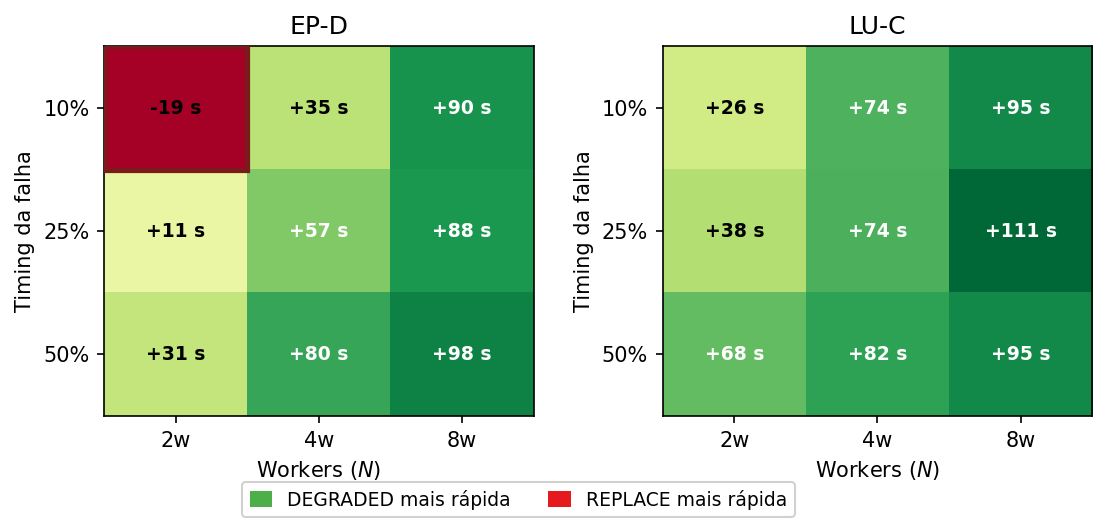
\includegraphics[width=\textwidth]{imgs/plots/fig10_crossover.png}
  \fonte{Elaborado pelo autor.}
\end{figure}

A leitura do mapa evidencia dois padrões. Primeiro, o fator dominante é o número de
\textit{workers}: as células ficam progressivamente mais escuras da esquerda para a
direita, refletindo a vantagem crescente da \textsc{Degraded} conforme $N$ aumenta.
Em 8~\textit{workers}, $\Delta$ fica entre $+$88 e $+$111~s independentemente do
momento da falha, porque perder um nó representa apenas $1/8$ da capacidade total e a
penalidade de P3 é pequena em comparação com a economia de P2b. Em
2~\textit{workers}, a margem é bem menor, pois a perda de um nó representa metade da
capacidade e a penalidade de P3 cresce substancialmente.

Segundo, dentro de cada coluna, o momento de falha também influencia a tendência:
falhas mais precoces (10\%, linha de cima) deixam mais trabalho para ser refeito com
$N{-}1$ \textit{workers}, aumentando a penalidade de P3 e reduzindo a vantagem da
\textsc{Degraded}. No EP-D, o tempo de execução mais longo resulta em valores de P3
maiores em termos absolutos, e esse efeito é suficiente para cruzar o ponto de inversão
a 2~\textit{workers} com falha a 10\%: a penalidade de P3 supera a economia de P2b e
a \textsc{Replace} vence ($\Delta = {-}19$~s, célula destacada em vermelho). Com
falha a 25\% ou 50\%, o trabalho restante já é menor e a \textsc{Degraded} volta a
ser mais rápida. No LU-C, o tempo de execução mais curto não gerou P3 suficientemente
grande para que a penalidade de P3 superasse a economia de P2b em nenhuma configuração,
e a \textsc{Degraded} vence em todos os cenários avaliados. Ainda assim, a tendência é
perfeitamente visível no mapa de calor: as células de LU-C a 2~\textit{workers}
apresentam os menores valores de $\Delta$ de todo o painel, indicando que um tempo de
execução maior já aproximaria o LU-C do ponto de inversão.

Para \textit{jobs} de longa duração ou com múltiplas falhas, a tendência se aprofunda.
O trabalho restante após uma falha cresce com a duração do \textit{job}; com volumes de
P3 substancialmente maiores do que os avaliados neste estudo, a penalidade da
\textsc{Degraded} superaria a economia de P2b mesmo em 8~\textit{workers}, tornando a
\textsc{Replace} a estratégia preferível. Além disso, este estudo modelou cenários com
apenas uma falha por execução. Na presença de múltiplas interrupções, a
\textsc{Degraded} perderia um \textit{worker} a cada evento, acumulando uma redução
progressiva de capacidade que amplificaria a penalidade de P3 a cada reinício.
A \textsc{Replace}, por repor sempre o nó interrompido, mantém a capacidade original
do \textit{cluster} independentemente do número de falhas, tornando-se mais robusta
nesse regime. A Seção~\ref{sec:overhead-ratio} examina as mesmas diferenças sob a
ótica de uma métrica de eficiência relativa.

\subsection{Razão de \textit{Overhead} de Recuperação}
\label{sec:overhead-ratio}

As seções anteriores mostraram que a vantagem da \textsc{Degraded} em tempo absoluto
($\Delta$) é maior nas falhas tardias e nos \textit{clusters} maiores, e tende a zero
conforme a falha ocorre mais cedo. Esta seção examina o mesmo fenômeno sob a ótica de
uma métrica normalizada: a razão de \textit{overhead} de recuperação,
$(T_{\text{total}} - P0) / T_{\text{total}}$, que mede qual fração do tempo total não
foi trabalho pré-falha preservado pelo \textit{checkpoint}. Ao normalizar pelo total,
a métrica permite comparar a eficiência relativa de cada estratégia independentemente
da duração absoluta do \textit{job}.

\begin{figure}[htb]
  \caption{Razão de \textit{overhead} de recuperação para EP-D e LU-C, por estratégia,
           número de \textit{workers} e momento da falha.}
  \label{fig:overhead-ratio}
  
\includegraphics[width=\textwidth]{imgs/plots/fig9_recovery_overhead_ratio.png}
  \fonte{Elaborado pelo autor.}
\end{figure}

\begin{table}[htb]
  \caption{Razão de \textit{overhead} de recuperação para o EP-D
           ($\%$, média $\pm$ dp, $N=3$).}
  \label{tab:overhead-ratio}
  \centering
  \begin{tabular}{l l c c c}
    \toprule
    Workers & Estratégia & 10\% & 25\% & 50\% \\
    \midrule
    2 & \textsc{Replace}  & $91{,}1 \pm 0{,}1$ & $78{,}6 \pm 0{,}5$ & $59{,}6 \pm 0{,}9$ \\
    2 & \textsc{Degraded} & $91{,}4 \pm 0{,}0$ & $78{,}2 \pm 0{,}2$ & $57{,}3 \pm 0{,}4$ \\
    \addlinespace
    4 & \textsc{Replace}  & $90{,}3 \pm 0{,}4$ & $77{,}4 \pm 0{,}1$ & $60{,}1 \pm 0{,}3$ \\
    4 & \textsc{Degraded} & $89{,}1 \pm 0{,}2$ & $73{,}2 \pm 0{,}2$ & $49{,}4 \pm 0{,}4$ \\
    \addlinespace
    8 & \textsc{Replace}  & $95{,}5 \pm 0{,}1$ & $88{,}5 \pm 0{,}6$ & $78{,}3 \pm 1{,}1$ \\
    8 & \textsc{Degraded} & $93{,}3 \pm 0{,}3$ & $83{,}0 \pm 0{,}1$ & $66{,}7 \pm 2{,}2$ \\
    \bottomrule
  \end{tabular}
  \fonte{Elaborado pelo autor.}
\end{table}

A Figura~\ref{fig:overhead-ratio} reproduz, sob a ótica normalizada, exatamente a
tendência identificada na Seção~\ref{sec:crossover}: quanto mais cedo a falha, mais
próximas as duas estratégias ficam. Com falha em 10\%, ambas apresentam razão entre
89\% e 96\% em qualquer tamanho de \textit{cluster}, praticamente indistinguíveis. A
explicação é a mesma do mapa de calor: falhas precoces deixam grande volume de
trabalho restante, e os totais de ambas as estratégias são dominados por esse P3
extenso. A economia de $\approx$\,109~s em P2b que a \textsc{Degraded} obtém
representa uma fração pequena de um total elevado e não se traduz em diferença relativa
significativa nesse regime. Isso corresponde diretamente ao fato de que as células da
coluna de 10\% no mapa de calor apresentam os menores valores de $\Delta$ de cada
linha.

Conforme a falha ocorre mais tarde (25\% e 50\%), o cenário muda da mesma forma
observada no mapa de calor: o P3 encolhe, o tempo total varia pouco, e os
$\approx$\,109~s economizados em P2b passam a representar uma fração crescente do
total. A vantagem relativa da \textsc{Degraded} se abre progressivamente, com a
diferença entre as razões das duas estratégias ampliando-se do centro para a direita
da figura. Em 4~\textit{workers} e falha em 50\%, a razão cai de 60\% na
\textsc{Replace} para 49\% na \textsc{Degraded}: mais da metade do tempo total desta
última foi computação pré-falha preservada pelo \textit{checkpoint}.

O caso mais resistente à melhora é a \textsc{Replace} em 8~\textit{workers}, onde a
razão permanece acima de 78\% mesmo com falha em 50\%. O motivo é estrutural: com
noFT de $\approx$\,99~s, a fase P2b da \textsc{Replace} ($\approx$\,128~s) já
supera o tempo total do \textit{job} sem instrumentação. Independentemente de quando a falha
ocorre, o provisionamento do nó substituto sozinho consome mais tempo do que o
\textit{job} levaria sem qualquer interrupção, tornando a razão de \textit{overhead}
estruturalmente alta. A \textsc{Degraded} escapa parcialmente desse efeito por manter
P2b em $\approx$\,11~s, mas a razão ainda não cai abaixo de 67\% em
8~\textit{workers}, refletindo a brevidade do próprio \textit{job} nessa escala. A
Seção~\ref{sec:custo} quantifica essa implicação em termos de custo financeiro na
nuvem.


\section{Análise de Custo}
\label{sec:custo}

As análises de tempo das seções anteriores mostraram quando cada estratégia termina
mais rápido. Esta seção complementa essa visão com a dimensão financeira: faz sentido
pagar por instâncias \textit{spot} e absorver o \textit{overhead} de recuperação para
obter um custo final menor do que o de uma execução noFT em instâncias
\textit{on-demand}?

O custo de cada cenário é estimado pelo produto entre o tempo total de execução e o
preço horário das instâncias utilizadas:
%
\begin{equation}
  \text{custo} = \frac{T}{3600}
    \bigl(p_{\text{workers}} \cdot N + p_{\text{head}}\bigr)
  \label{eq:cost}
\end{equation}
%
em que $T$ é o tempo total em segundos, $N$ é o número de \textit{workers} e
$p_{\text{head}} = \$0{,}0832/\text{h}$ é o preço do coordenador, sempre
\textit{on-demand}. O que difere entre o cenário noFT e os cenários FT é o preço
dos \textit{workers}: $p_{\text{workers}} = \$0{,}1920/\text{h}$ para o noFT
(instâncias \textit{on-demand}) e $p_{\text{workers}} = \$0{,}0585/\text{h}$ para as
estratégias FT (instâncias \textit{spot}). Esse desconto de $\approx$70\% sobre o
componente dos \textit{workers} é o crédito que cada estratégia dispõe para
compensar o tempo adicional introduzido pelo \textit{overhead} de recuperação. A
Figura~\ref{fig:cost} e a Tabela~\ref{tab:cost} exibem os resultados.

\begin{figure}[htb]
  \caption{Custo estimado por \textit{benchmark}, tamanho de \textit{cluster}
           e estratégia.}
  \label{fig:cost}
  
\includegraphics[width=\textwidth]{imgs/plots/fig7_cost.png}
  \fonte{Elaborado pelo autor.}
\end{figure}

\begin{table}[htb]
  \caption{Custo estimado por execução (USD) e economia relativa ao noFT
           \textit{on-demand} (médias sobre os três momentos de falha; positivo
           indica economia, negativo indica acréscimo).}
  \label{tab:cost}
  \centering
  \small
  \begin{tabular}{l c r r r r r}
    \toprule
    & & &
      \multicolumn{2}{c}{\textsc{Replace} \textit{spot}} &
      \multicolumn{2}{c}{\textsc{Degraded} \textit{spot}} \\
    \cmidrule(lr){4-5} \cmidrule(lr){6-7}
    Benchmark & Workers & noFT & Custo & Eco.~(\%) & Custo & Eco.~(\%) \\
    \midrule
    CG-C & 2 & \$0,0044 & \$0,0115 & $-$161 & \$0,0094 & $-$112 \\
    CG-C & 4 & \$0,0048 & \$0,0173 & $-$260 & \$0,0082 & $-$71  \\
    CG-C & 8 & \$0,0055 & \$0,0311 & $-$465 & \$0,0148 & $-$170 \\
    \addlinespace
    EP-D & 2 & \$0,0434 & \$0,0303 & $+$30  & \$0,0298 & $+$31  \\
    EP-D & 4 & \$0,0401 & \$0,0313 & $+$22  & \$0,0263 & $+$34  \\
    EP-D & 8 & \$0,0446 & \$0,0419 & $+$6   & \$0,0278 & $+$38  \\
    \addlinespace
    LU-C & 2 & \$0,0192 & \$0,0193 & $-$1   & \$0,0168 & $+$12  \\
    LU-C & 4 & \$0,0196 & \$0,0238 & $-$21  & \$0,0170 & $+$13  \\
    LU-C & 8 & \$0,0214 & \$0,0365 & $-$71  & \$0,0211 & $+$2   \\
    \bottomrule
  \end{tabular}
  \fonte{Elaborado pelo autor.}
\end{table}

O ponto de partida é o CG-C, onde nenhuma estratégia produz economia em nenhuma
configuração. Isso já era antecipado pela análise de \textit{overhead} da
Seção~\ref{sec:overhead}: o tempo de recuperação supera o próprio tempo de cálculo
do \textit{job}, de modo que pagar pelo desconto \textit{spot} em instâncias que
rodam 3 a 17 vezes mais tempo do que o necessário não produz vantagem alguma. Essa
constatação, porém, levanta a questão inversa: a partir de qual duração o desconto
passa a compensar?

A resposta emerge ao percorrer as colunas de economia da tabela do CG-C para o LU-C
e depois para o EP-D. Em ambas as estratégias, a economia cresce com a duração do
\textit{benchmark}: o \textit{overhead} de recuperação tem custo fixo no tempo;
quanto maior $T$, menor a fração que ele representa sobre o custo total, e maior a
proporção efetivamente coberta pelo desconto \textit{spot}. A \textsc{Degraded} torna
essa tendência mais visível porque seu P2b de $\approx$11~s é quase desprezível: seu
custo reflete, de forma mais direta, o efeito do desconto sobre o tempo de execução.
No LU-C, a \textsc{Degraded} já alcança economia positiva em todas as configurações
(+12\%, +13\% e +2\%); no EP-D, essa economia sobe para a faixa de 31\% a 38\%.

A \textsc{Replace} segue a mesma direção, mas com um peso adicional: seu P2b de
$\approx$120~s corresponde ao período de reprovisionamento da AWS, durante o qual
nenhum cálculo é realizado, mas todas as instâncias continuam sendo faturadas. No
LU-C, esse custo de espera é o que separa as duas estratégias: enquanto a
\textsc{Degraded} já opera no positivo, a \textsc{Replace} ainda fica no negativo
($-$1\% e $-$21\%). Contudo, como esse P2b é constante, independente do número de
\textit{workers} e do \textit{benchmark}, ele pesa cada vez menos à medida que a
duração do \textit{job} cresce. No EP-D, o \textit{benchmark} de maior tempo de
execução neste estudo, a \textsc{Replace} recupera viabilidade e as economias das
duas estratégias convergem para valores praticamente iguais, de 30\% e 31\% em
2~\textit{workers}. Esse comportamento econômico é análogo ao que foi observado na
Seção~\ref{sec:crossover} em termos de tempo: quanto maior o trabalho restante, mais
a \textsc{Replace} se aproxima da \textsc{Degraded}.

Observando agora o efeito do tamanho do \textit{cluster}, nota-se que tanto a
\textsc{Replace} quanto a \textsc{Degraded} apresentam custos relativamente similares
entre 2 e 4~\textit{workers}, mas com aumento mais expressivo ao passar para
8~\textit{workers}. Para a \textsc{Replace}, a explicação é direta: cada
\textit{worker} adicional também paga durante o P2b, fazendo o custo de espera crescer
linearmente com $N$, o que é mais notável em configurações de menor duração como o
LU-C e o CG-C. Para a \textsc{Degraded}, o aumento ao passar para 8~\textit{workers}
é visível em LU-C e CG-C, mas quase não ocorre no EP-D: o custo de 4 para
8~\textit{workers} passa de \$0{,}0263 para \$0{,}0278 (+6\%), enquanto a economia
melhora de 34\% para 38\%. Uma explicação plausível, derivada da
Equação~\ref{eq:cost}, é que os \textit{workers} \textit{on-demand} do noFT são
proporcionalmente mais caros por hora que os \textit{spot} do FT; adicionar mais
\textit{workers} tenderia a encarecer o noFT mais do que a \textsc{Degraded},
ampliando a diferença relativa. Esse efeito, se presente, só se traduz em melhora
de economia no EP-D porque nele o desconto \textit{spot} já parte de uma posição
positiva; nos \textit{benchmarks} mais curtos, o \textit{overhead} ainda domina e a
variação relativa não é suficiente para alterar o sinal do resultado.


\section{Discussão}
\label{sec:discussao}

Ao longo deste capítulo, a decomposição em fases P0--P3 revelou onde o tempo de
um \textit{job} com falha é efetivamente gasto. Da análise das fases emerge que
as estratégias divergem em dois componentes: P2b, a reconfiguração do nó após a
detecção da falha, e P3, a computação pós-reinício. A \textsc{Degraded} conclui
P2b em $\approx$11~s ao atualizar apenas o estado do nó no Slurm, mas retoma a
execução em P3 com $N{-}1$ \textit{workers}, acumulando uma penalidade proporcional
ao trabalho remanescente. A \textsc{Replace}, inversamente, aguarda $\approx$120~s
em P2b pelo reaprovisionamento de um nó substituto na AWS, mas retoma com a
capacidade integral do \textit{cluster} em P3. O resultado dessa oposição é
determinado por
dois fatores que interagem: o número de \textit{workers} ($N$) e o volume de
trabalho presente no momento da falha. Em \textit{clusters} maiores, a perda de
um nó representa uma fração cada vez menor da capacidade total, reduzindo a
penalidade de P3 da \textsc{Degraded} e tornando a economia de P2b dominante. Em
\textit{clusters} pequenos com falha precoce, o peso de P3 pode superar os 109~s
economizados, tornando a \textsc{Replace} mais rápida, situação observada apenas
no EP-D com 2~\textit{workers} e falha a 10\% do tempo total. O mapa de calor da
Seção~\ref{sec:crossover} torna essa estrutura visível de forma direta.

Esse mecanismo de compensação pressupõe que a duração do \textit{job} seja
suficiente para que o \textit{overhead} de recuperação represente uma fração
minoritária do tempo total. Para \textit{jobs} curtos como o CG-C, nenhuma das
estratégias produz resultado favorável: o \textit{overhead} equivale a 3--17
vezes o tempo útil de cálculo, e o desconto \textit{spot} não compensa, seja em
tempo seja em custo. Para \textit{jobs} de duração moderada a longa como o EP-D
e o LU-C, a balança se inverte: a \textsc{Degraded} alcança economia de 2 a 38\%
em relação ao noFT \textit{on-demand}, e as análises de tempo e de custo apontam
consistentemente na mesma direção em todos os cenários avaliados. Um achado
complementar nesse regime é a aceleração sistemática de P3 na \textsc{Replace}:
em todos os cenários do EP-D e do LU-C, o P3 observado ficou entre 5 e 34\%
abaixo do valor esperado com base no tempo MANA-noFT, sugerindo que o reinício
a quente em \textit{cluster} íntegro beneficia o desempenho de formas que os
dados disponíveis não permitem isolar completamente.

Três aspectos delimitam o escopo dos resultados. Os experimentos cobriram apenas
cenários de falha única: com falhas múltiplas, a \textsc{Degraded} degrada
progressivamente a capacidade do \textit{cluster}
($N \rightarrow N\!-\!1 \rightarrow N\!-\!2$), enquanto a \textsc{Replace}
recompõe o nó a cada evento e preserva a capacidade original, tornando-se mais
robusta nesse regime. O intervalo de duração testado foi de 12 a 500~s; o
regime de aplicações longas, em que a amortização do \textit{overhead} de
recuperação seria ainda mais pronunciada, foi discutido analiticamente mas não
validado empiricamente. Por fim, os tempos de P1 e P2b observados são específicos
à instância m5.xlarge e ao Amazon EFS; variações nesses componentes de
infraestrutura deslocariam o ponto de equilíbrio entre as estratégias de forma
direta.


\section{Ameaças à Validade}
\label{sec:ameacas-validade}

Esta seção sistematiza os fatores que podem limitar a generalização dos resultados
apresentados, distinguindo ameaças à validade interna das ameaças à validade externa.

A principal ameaça à \textbf{validade interna} é o uso de injeção sintética de
falhas em substituição a revogações reais da AWS. O mecanismo
\texttt{auto\_test\_failure} termina a instância alvo após um intervalo configurável,
replicando o comportamento da janela de aviso \textit{spot}, mas não cobre situações em
que a revogação ocorre durante a fase P1 de escrita do \textit{checkpoint} ou em
momentos de sincronização interna do MANA. A reprodutibilidade controlada viabiliza a
comparação entre estratégias, mas pode subestimar o impacto de revogações em momentos
desfavoráveis ao \textit{checkpoint}.

As principais ameaças à \textbf{validade externa} dizem respeito à cobertura
experimental. Os três \textit{benchmarks} selecionados, CG-C, EP-D e LU-C, foram
escolhidos por representarem perfis de comunicação distintos, mas não esgotam o espaço
de aplicações MPI: padrões como comunicações coletivas densas, topologias de grafo
irregular ou \textit{stencils} de múltiplos vizinhos podem exibir \textit{overhead} e
sensibilidade às estratégias diferentes dos observados nos cenários avaliados. A avaliação
utilizou exclusivamente instâncias m5.xlarge como \textit{workers} e Amazon EFS como
sistema de arquivos compartilhado em uma única região da AWS; latências de P1 e P2b são
específicas a essa combinação de infraestrutura, e variações em tipo de instância,
sistema de armazenamento ou provedor de nuvem deslocariam os valores absolutos e, por
consequência, o ponto de equilíbrio entre as estratégias. Por fim, os experimentos
modelaram exclusivamente cenários de falha única; o comportamento das estratégias sob
falhas múltiplas e simultâneas, relevante em ambientes com alta taxa de revogação,
não foi avaliado empiricamente.

% ==========================================================================
\chapter{Conclusão}
\label{ch:conclusao}
% ==========================================================================

Este capítulo sintetiza as contribuições do trabalho e aponta caminhos para investigação
futura. A Seção~\ref{sec:consideracoes-finais} retoma os objetivos estabelecidos na
introdução e avalia em que medida foram atendidos. A Seção~\ref{sec:trabalhos-futuros}
identifica extensões derivadas das limitações e fenômenos em aberto encontrados ao
longo da avaliação.

\section{Considerações Finais}
\label{sec:consideracoes-finais}

A motivação deste trabalho partiu de uma tensão operacional concreta: instâncias
\textit{spot} da AWS oferecem descontos de até 90\% em relação ao preço convencional,
mas a possibilidade de revogação a qualquer momento, com apenas dois minutos de aviso,
inviabiliza seu uso direto para aplicações MPI de longa duração sem proteção de estado.
A pergunta central que organizou o trabalho foi se é possível executar aplicações MPI
legadas de forma resiliente e economicamente vantajosa em instâncias \textit{spot}, sem
exigir modificação do código das aplicações. A resposta construída ao longo dos
capítulos foi afirmativa, com a ressalva de que a viabilidade depende de forma
determinante da duração do \textit{job}.

O primeiro passo foi estabelecer a topologia adequada para o \textit{cluster}. O
Capítulo~\ref{ch:burstable} mostrou que instâncias \textit{burstable} T3 são
inadequadas para \textit{workers} HPC com comunicação intensiva: em \textit{benchmarks}
de sincronização contínua como o LU, a conjugação de esgotamento de créditos de CPU e
largura de banda de rede restrita resultou em execuções até três vezes mais lentas do
que o equivalente M5. O mesmo capítulo identificou o ponto de adequação dessas
instâncias: cargas intermitentes com baixo tráfego de rede, como o \textit{coordinator}
de \textit{checkpoint} do MANA. Esse resultado fundamentou diretamente a topologia
híbrida adotada, na qual o \textit{head} opera como instância t3.large
\textit{on-demand} e os \textit{workers} executam como m5.xlarge \textit{spot},
combinando imunidade a preempções no coordenador com custo reduzido nos nós de cálculo.

Sobre essa topologia, o Capítulo~\ref{ch:implementacao} descreveu a integração com
o HPC@Cloud: \textit{bootstrap} automatizado do ambiente Slurm e MANA,
mecanismo de detecção reativa de interrupções por consulta periódica à API \textit{spot}
da EC2, e dois modelos de recuperação transparentes para a aplicação. A
\textsc{Replace} repõe o nó interrompido e retoma o \textit{job} com a capacidade
original do \textit{cluster}; a \textsc{Degraded} marca o nó como inativo e continua
imediatamente com $N{-}1$ \textit{workers}, trocando paralelismo por latência de
recuperação. A instrumentação em fases P0--P3 foi projetada para isolar cada componente
do custo de recuperação, separando tempo de computação de tempo de infraestrutura e de
coordenação, e tornando possível a análise estrutural conduzida no
Capítulo~\ref{ch:avaliacao}.

A avaliação experimental, conduzida com 282 execuções sobre os \textit{benchmarks} NPB
CG-C, EP-D e LU-C em \textit{clusters} de 2, 4 e 8 \textit{workers}, revelou que o
\textit{overhead} do MANA em condições normais é aplicação-dependente: varia de 27\%
no EP-D com 8~\textit{workers} a 222\% no CG-C com 2~\textit{workers}. Os estudos
sintéticos identificaram que a frequência de chamadas MPI não é o mecanismo
amplificador; o custo intrínseco medido em programas isolados é de apenas 4 a 5~s por
execução, associado à inicialização e finalização do processo. A distância entre esse
valor e os percentuais dos \textit{benchmarks} reais indica que o \textit{overhead}
relevante emerge da interação entre o padrão de execução de cada aplicação e a camada
do MANA, com o CG-C em 2~\textit{workers} como caso extremo atribuído a uma hipótese
de desbalanceamento de carga ainda não confirmada instrumentalmente.

Em cenários com falha, a comparação entre estratégias é estruturada pela fase P2b, que
compreende a reconfiguração do nó após a detecção da falha: a \textsc{Degraded} conclui
essa fase em $\approx$11~s ao atualizar o estado no Slurm, enquanto a \textsc{Replace}
aguarda $\approx$120~s pelo reaprovisionamento de um nó substituto na AWS. Esse
diferencial, combinado com a penalidade de capacidade reduzida em P3, cria uma estrutura
de \textit{crossover} em que o vencedor depende do tamanho do \textit{cluster} e do
volume de trabalho presente no momento da falha: quanto menor o \textit{cluster} e mais
precoce a falha, mais competitiva se torna a \textsc{Replace}. Essa mesma lógica
estrutural se reflete na dimensão financeira: o desconto de $\approx$70\% das instâncias
\textit{spot} supera o custo de recuperação em \textit{jobs} de duração moderada a
longa, com as análises de tempo e de custo convergindo para a mesma conclusão em todos
os \textit{benchmarks} avaliados e economia de 2 a 38\% sobre o equivalente
\textit{on-demand} sem recuperação.

Nos cenários avaliados, a integração construída demonstra que execução resiliente e
econômica de aplicações MPI legadas em instâncias \textit{spot} é alcançável, desde que
a duração do \textit{job} seja suficiente para que o custo fixo de recuperação represente
uma fração minoritária do tempo total. Para \textit{jobs} muito curtos, como o CG-C, o
\textit{overhead} domina e a solução não se justifica; para \textit{jobs} de duração
moderada a longa, como os EP-D e LU-C avaliados, a solução proposta produziu execuções
confiáveis a custo reduzido nas condições experimentais deste estudo. Os seis objetivos
específicos estabelecidos na Seção~\ref{sec:objetivos} foram atendidos: a análise de
viabilidade de instâncias \textit{burstable} fundamentou a topologia adotada; o
HPC@Cloud foi estendido com suporte à arquitetura híbrida, ao \textit{bootstrap}
automatizado e aos mecanismos de recuperação; e a avaliação experimental quantificou o
\textit{overhead}, caracterizou o comportamento das estratégias e identificou as
condições de viabilidade econômica.

\section{Trabalhos Futuros}
\label{sec:trabalhos-futuros}

A avaliação empírica cobriu \textit{jobs} de 12 a 500~s; a inversão prevista
estruturalmente entre estratégias, na qual o custo acumulado de P3 da \textsc{Degraded}
com $N{-}1$ \textit{workers} superaria a economia de P2b, não foi observada
experimentalmente. Confirmar esse \textit{crossover} demandaria classes mais custosas
dos \textit{benchmarks}, como o LU-D ou o EP-E. Uma restrição operacional relevante
nesse contexto é o limite de dois minutos entre o aviso de revogação da AWS e a
terminação da instância: aplicações com \textit{footprint} de memória por processo
elevado podem não conseguir concluir a escrita do \textit{checkpoint} dentro dessa
janela, tornando o mecanismo de recuperação inviável independentemente da duração do
\textit{job}. A identificação do limiar de \textit{footprint} a partir do qual a fase
P1 excede o tempo disponível é, portanto, uma condição prévia para a extensão da
avaliação a classes superiores.

Os experimentos modelaram exclusivamente cenários de falha única por execução. Em
ambientes com alta taxa de interrupção de instâncias \textit{spot}, falhas múltiplas e
sequenciais são cenários realistas: na \textsc{Degraded}, cada evento reduz
progressivamente a capacidade computacional do \textit{cluster}
($N \rightarrow N\!-\!1 \rightarrow N\!-\!2$), o que pode inviabilizar a conclusão do
\textit{job} em casos extremos. A avaliação do comportamento das estratégias sob
múltiplas falhas, e a definição de um limiar mínimo de $N$ abaixo do qual a
\textsc{Degraded} deixa de ser viável, constitui uma extensão natural do trabalho.
Associado a isso, o mecanismo de recuperação atual processa falhas de forma sequencial;
o suporte a recuperações paralelas, para o caso de múltiplos \textit{workers}
interrompidos ao mesmo tempo, reduziria o impacto dessas situações sobre o tempo total
de execução.

O mecanismo de \textit{checkpoint} implementado é estritamente reativo: é acionado
apenas quando sinais de preempção são detectados. Uma extensão em duas etapas ampliaria
a robustez do sistema. No curto prazo, a adição de \textit{checkpoints} periódicos
automáticos limitaria o retrabalho em interrupções que ocorrem antes da janela de aviso.
Em uma etapa seguinte, a incorporação de técnicas de predição de revogações com base em
histórico de interrupções de instâncias \textit{spot} permitiria antecipar o disparo do
\textit{checkpoint} em instâncias com maior risco iminente, combinando a reatividade do
mecanismo atual com uma camada proativa de proteção de estado.

Dois fenômenos identificados na avaliação experimental permanecem sem caracterização
completa. O \textit{overhead} anômalo do CG-C com 2~\textit{workers} ($+$222\%, contra
55 a 71\% nas configurações de 4 e 8~\textit{workers}) foi hipotetizado como causado
pela co-localização de processos e o laço ativo do MANA no \texttt{MPI\_Wait}, mas a
hipótese não foi confirmada por instrumentação interna do \textit{benchmark};
\textit{profiling} por \textit{rank} permitiria verificar se o padrão de espera amplifica
o \textit{overhead} nessa configuração específica. A aceleração de P3 na
\textsc{Replace}, entre 5 e 34\% mais rápida do que o previsto pelo tempo
MANA-noFT, constitui um fenômeno sistemático observado em todos os cenários avaliados
para EP-D e LU-C, sem explicação identificável a partir dos dados disponíveis;
contadores de eventos de hardware poderiam revelar o mecanismo subjacente. A
caracterização desses dois comportamentos contribuiria para a compreensão do MANA em
condições reais e para o refinamento dos modelos de estimativa de custo de recuperação.


%%% Local Variables:
%%% mode: latex
%%% TeX-master: "main"
%%% End:

\postextual
\bibliography{main}
% Assume-se que \postextual já foi feito

%%% Apêndices — descomentar e preencher conforme necessário
% \apendices
%
% \chapter{Configurações dos Experimentos}
% \label{ch:apendice-configs}
% TODO: incluir os YAMLs de cluster e task usados nos experimentos
%       (head t3.large + 4× m5.xlarge spot, task com auto_test_failure).
%
% \chapter{Resultados Completos}
% \label{ch:apendice-resultados}
% TODO: tabelas com todos os 94 runs se não couberem no corpo principal.

\imprimirindice

%%% Local Variables:
%%% mode: latex
%%% TeX-master: "main"
%%% End:


\end{document}
